\documentclass[a4paper, table]{article}

\usepackage{xcolor}
\usepackage{amssymb}
\usepackage[english]{babel}
\usepackage[a4paper]{geometry}
\usepackage[T1]{fontenc}
\usepackage[utf8]{inputenc}
\usepackage{graphicx}
\usepackage{todonotes}
\usepackage{hyperref}
\usepackage{longtable}
\usepackage{times}
\usepackage{pdflscape}
\usepackage[style=verbose-ibid,backend=bibtex]{biblatex}
\usepackage{listings}
\usepackage[
    automark,
    autooneside=false,% <- needed if you want to use \leftmark and \rightmark in a onesided document
    headsepline
]{scrlayer-scrpage}
% https://tex.stackexchange.com/questions/8946/how-to-combine-acronym-and-glossary
\usepackage[acronym]{glossaries}
%\usepackage{glossaries}
%\usepackage[automake]{glossaries-extra}

% Replace "Glossary" with "II   Glossar"
% https://www.mrunix.de/forums/showthread.php?65522-Glossaries-Verzeichnisbezeichnungen-umbenennen
% using english because german needs an extra package installed
\addto\captionsenglish{
    \renewcommand\glossaryname{II{\hspace*{1cm}}Glossar}
}
\deftranslation[to=english]{Glossary}{II{\hspace*{1cm}}Glossar}

%\makeglossaries
%\makeglossary
\makenoidxglossaries

% https://tex.stackexchange.com/questions/8946/how-to-combine-acronym-and-glossary
\newglossaryentry{STAIR}
{
    name={STAIR},
    description={(Students Association Informatics Rotkreuz) Der Studierendenverein des Departement Informatik der Hochschule Luzern.}
    long={Students Association Informatics Rotkreuz}
}
\newglossaryentry{URL}
{
    name={URL},
    description={(Uniform Resource Locator) Mit URL wird eine Adresse bezeichnet, die den Pfad auf eine Datei, auf einem gewissen Server angibt.},
    long={Uniform Resource Locator}
}
\newglossaryentry{REST}
{
    name={REST},
    description={(Representational State Transfer) Programmierparadigma, welches das Verhalten für Kommunikation im Web zwischen Client und Server beschreibt.},
    long={Representational State Transfer}
}
\newglossaryentry{API}
{
    name={API},
    description={(Application Programming Interface) Ein API beschreibt eine Programmierschnittstelle, an die ein anderes Program Anfragen schicken kann, um Daten auszutauschen oder eine Funktion zu starten.},
    long={Application Programming Interface}
}
\newglossaryentry{SoDa}
{
    name={SoDa},
    description={(Software Development Agile) SoDa beschreibt ein Scrum basiertes Projekt- und Vorgehensmodell für die Forschung und Industrie. Es wird vor allem in der Softwareentwicklung gebraucht.},
    long={Software Development Agile}
}
\newglossaryentry{CSV}
{
    name={CSV},
    description={(Comma Separated Values) Es beschreibt ein Dateiformat, bei dem die Daten kommasepariert sind.}
    long={Comma Separated Values}
}
\newglossaryentry{JSON}
{
    name={JSON},
    description={(JavaScript Object Notation) Es beschreibt ein Datenaustauschformat.}
    long={JavaScript Object Notation}
}
\newglossaryentry{bzw.}
{
    name={bzw.},
    description={beziehungsweise}
}
\newglossaryentry{z.B.}
{
    name={z.B.},
    description={zum Beispiel}
}
% Deployment
% Discord
% HSLU
% ISA Module
% Konsolenanwendungen
% REST
% Windows-Subsystem for Linux = WSL
%\newacronym

\definecolor{dkgreen}{rgb}{0,0.6,0}
\definecolor{gray}{rgb}{0.5,0.5,0.5}
\definecolor{mauve}{rgb}{0.58,0,0.82}

\lstset
{
    frame=none,
    basicstyle={\small\ttfamily},
    commentstyle=\color{dkgreen},
    stringstyle=\color{mauve},
    numbers=none, %Nummerierung
    numberstyle=\tiny\color{gray},
    showstringspaces=false,
    breaklines=true,
    aboveskip=3mm,
    belowskip=3mm,
    columns=flexible,
    breakatwhitespace=true
}

\lstdefinelanguage{csharp}
{
    language=[Sharp]C,
    keywordstyle=\color{blue},
    tabsize=3,
    morekeywords={partial, var, value, get, set}
}

\lstdefinelanguage{json}
{
    stepnumber=1,
    numbersep=8pt,
    string=[s]{"}{"},
    comment=[l]{:\ "},
    morecomment=[l]{:"},
    literate=
        *{0}{{{\color{numb}0}}}{1}
         {1}{{{\color{numb}1}}}{1}
         {2}{{{\color{numb}2}}}{1}
         {3}{{{\color{numb}3}}}{1}
         {4}{{{\color{numb}4}}}{1}
         {5}{{{\color{numb}5}}}{1}
         {6}{{{\color{numb}6}}}{1}
         {7}{{{\color{numb}7}}}{1}
         {8}{{{\color{numb}8}}}{1}
         {9}{{{\color{numb}9}}}{1}
}

\lstdefinestyle{XML}
{
    morestring=[b]",
    moredelim=[s][\bfseries\color{green}]{<}{\ },
    moredelim=[s][\bfseries\color{green}]{</}{>},
    moredelim=[l][\bfseries\color{green}]{/>},
    moredelim=[l][\bfseries\color{green}]{>},
    morecomment=[s]{<?}{?>},
    morecomment=[s]{<!--}{-->},
    identifierstyle=\color{blue}
}

\hypersetup{
    colorlinks=true,
    linkcolor=darkgray,
    filecolor=magenta,
    urlcolor=blue
}
\urlstyle{same}

\bibliography{wipro-main-doc}
\graphicspath{ {images/} }

\newcommand{\tabitem}{~~\llap{\textbullet}~~}
\newcommand{\rot}{\rotatebox{90}}

% Set name of image label
\renewcommand{\figurename}{Abbildung}

\title{
    {Wirtschaftsprojekt} \\
    \vspace{10mm}
    { Herbstsemester 2022 } \\
    \vspace{10mm}
    % https://commons.wikimedia.org/wiki/File:HSLU_2022_logo.svg
    {
\includegraphics[width=75mm]{img/hsluLogo2022.png}}
}

\author{Yannis Kr\"amer und Nicolas Wiedmer}
\date{23.12.2022}

\begin{document}

\maketitle

% Set header
\clearpairofpagestyles
\ihead{WIPRO - STAIR Discord Bot}
\ohead{\leftmark}
%\ohead{\ifstr{\leftmark}{\rightbotmark}{}{\rightbotmark}}
\cfoot*{\pagemark}
\renewcommand*\thispagestyle{scrheadings}% default pagestyle

\newpage

\noindent
\fontsize{12}{14}
\textbf{Wirtschaftsprojekt an der Hochschule Luzern -- Informatik} \\ \vspace*{0.6cm}

\fontsize{10.95}{12}
\noindent
\textbf{Titel:} STAIR Discord Bot \\ \vspace*{0.2cm}

\noindent
\textbf{Studentin/Student:} Yannis Kr\"amer \newline \newline
\textbf{Studentin/Student:} Nicolas Wiedmer \newline \newline
\textbf{Studiengang:} BSc Informatik oder Wirtschaftsinformatik  \newline \newline
\textbf{Jahr:} 2022 \newline \newline
\textbf{Betreuungsperson:} Markus Waldmann \newline \newline
\textbf{Expertin/Experte:} \newline \newline
\textbf{Auftraggeberin/Auftraggeber:} STAIR (Martin Steiger \& Estefania Otero)\newline \newline \newline
\textbf{Codierung / Klassifizierung der Arbeit:}\\
$\boxtimes$ \"Offentlich
$\square$ Vertraulich


%%% you can use \boxtimes for filling a cross inside the square
%%% e.g., $\boxtimes$ A: Einsicht 	(Normalfall)


\paragraph{\textbf{Eidesstattliche Erkl\"arung}}
Ich erkl\"are hiermit, dass ich/wir die vorliegende Arbeit selbst\"andig und ohne unerlaubte fremde Hilfe angefertigt haben, alle verwendeten Quellen, Literatur und andere Hilfsmittel angegeben haben, w\"ortlich oder inhaltlich entnommene Stellen als solche kenntlich gemacht haben, das Vertraulichkeitsinteresse des Auftraggebers wahren und die Urheberrechtsbestimmungen der Hochschule Luzern respektieren werden. \newline \newline
Ort / Datum, Unterschrift	\underline{\hspace*{8cm}} \newline \newline
Ort / Datum, Unterschrift	\underline{\hspace*{8cm}} \newline \newline \newline
\textbf{Ausschliesslich bei Abgabe in gedruckter Form: \\
Eingangsvisum durch das Sekretariat auszuf\"ullen}\newline \newline
Rotkreuz, den	\underline{\hspace*{4cm}}	\hspace*{1cm} Visum:	\underline{\hspace*{4cm}}

\normalfont
\newpage
\section*{I{\hspace*{1cm}}Abstract}
Der Studierendeverein \gls{STAIR} der Hochschule Luzern betreibt einen Discord Server, auf dem sich die Studierenden austauschen können. 
Auf dem Server laufen 2 Bots, die sich um die Authentifikation und die Anmeldung für Modul-Channels kümmern. 
Die Bots funktionieren nicht zusammen und es kommt bei der Modul-Channel-Anmeldung immer wieder zu Problemen.\\
Das Ziel dieser Arbeit ist es, den Discord Bot des Studierendevereins STAIR neu zu implementieren, um die Administrationsarbeit auf dem Server zu verringern und neue Daten für Event- und Marketingplanung zu sammeln.\\
Dabei wird mithilfe einer Ist-Analyse der alte Bot untersucht und Änderungsentscheidungen getroffen. 
Diese Änderungen werden im Verlauf von 5 Sprints nach der Software-Development-Agile \gls{SoDa} Methode implementiert.\\
Es wird ein neuer Bot erstellt, welcher den Authentifizierungsmechanismus und verschiedene Befehle für STAIR Mitglieder und Studierende beinhaltet. 
Des Weiteren wird eine Datenbank aufgebaut, sowie der Bot auf einem Linux Server in der Hochschul-Enterprise-Lab Umgebung eingesetzt. 
Für den operativen Einsatz wird eine Anleitung geschrieben, die den Administratoren des Discord Servers eine Hilfe bei der Aktualisierung der Studierenden und der Module jedes Semesters bietet. \\
Für die Studierenden wird der Discord Server übersichtlicher gestaltet und der Umgang mit dem Bot vereinfacht. 
Mithilfe des Bots können in Zukunft neue Studierende auf dem Discord Server einfacher verwaltet werden. 
Durch die Einführung einer Datenbank erhalten STAIR Mitglieder die Möglichkeit, Events- und Marketingkampagnen besser auf bestimmte Zielgruppen anzupassen.\\\\

\textit{
    The student association STAIR of the Lucerne University of Applied Sciences and Arts operates a Discord server on which students can exchange information. 
    There are 2 bots running on the server that take care of authentication and registration for module channels. 
    The bots do not work together and there are always problems with the module channel registration.\\
    The goal of this work is to re-implement the Discord bot of the student club STAIR to reduce the administration work on the server and to collect new data for event and marketing planning.
    With the help of an as-is-analysis, the old bot will be examined and change-decisions will be made.
    These changes are implemented over the course of 5 sprints using the software development Agile \gls{SoDa} method.\\
    A new bot will be created, which will include the authentication mechanism and various commands for STAIR members and students. 
    Furthermore, a database will be built and the bot will be deployed on a Linux server in the university enterprise lab environment. 
    For operational use, a guide will be written to assist Discord server administrators in updating students and modules each semester. \\
    For the students, the Discord server will be more clearly arranged and the handling of the bot will be simplified. 
    With the help of the bot, it will be easier to manage new students on the Discord server in the future. 
    The introduction of a database will give STAIR members the ability to better tailor event and marketing campaigns to specific audiences.}

\newpage
\printnoidxglossaries

% https://blog.aristolo.com/de/definition-begriffe-bachelorarbeit-masterarbeit-dissertation/

\newpage
\tableofcontents

\newpage

\section{Problem, Fragestellung, Vision}
Der Studierendeverein STAIR des Departments Informatik der Hochschule Luzern stellt über die Plattform Discord einen Server zur Verfügung. 
Über diesen können sich Studierende über das Studium oder spezifische Module austauschen.\\
Auf dem Server laufen zwei Bots, welche sich um die Authentifikation der Studierenden sowie um die Einschreibung in die verschiedenen Modul-Channels kümmern. 
Der Bot zur Authentifikation funktioniert einwandfrei, jedoch kommt es beim Bot zur Moduleinschreibung immer wieder zu Problemen. 
Da dieser extern auf einer Plattform namens Nadeko erstellt wurde, kann nicht genau gesagt werden, wieso diese Probleme auftreten.\\
Des Weiteren gibt es Unklarheiten bei den Studierenden zur Benutzung dieser Bots. 
Auch die Aufteilung der Modul-Channels in verschiedene Kategorien ist nicht benutzerfreundlich gestaltet. 
In einer neuen Version sollen die Probleme beseitigt und die Unklarheiten bei die Studierenden geklärt werden.\\\\
In diesem Projekt soll eine Lösung entwickelt werden, die den Discord Administratoren von STAIR eine Unterstützung und Mehrwert bietet. 
Die Lösung soll für STAIR und Studierende verständlich sein und einfach eingesetzt werden können.\\\\
Das Ziel der Arbeit ist es, die vorher beschriebenen zwei Bots zusammenzuführen und damit eine einheitliche Plattform zu schaffen, über welche Bot Commands verwaltet werden. 
Weiter soll eine Datenbank eingeführt werden, die Studierende und Ihre Discord Accounts verbindet. 
Dies erleichtert die Authentifikation und die Verwaltung der Modul-Channels. 
Die Daten bieten ebenfalls einen statistischen Mehrwert für die STAIR Mitglieder, da ein besser Einblick gewährt wird, wer den Discord Server nutzt. 
Dies kann für Marketingzwecke sowie Event-Planung verwendet werden.\\
Auch soll der Einsatz von einer automatischen Fehlererkennung dazu beitragen, dass Probleme beim Bot schnell an die Administratoren von STAIR weitergeleitet werden. 
So können lange Unsicherheiten und Probleme schneller behoben werden. 
Der Einsatz einer neuen Logging-Library soll die Nachvollziehbarkeit der Software sicherstellen. 
Diese Einträge sollen die Administratoren beim allfälligen Fehlersuchen unterstützen.


\newpage
\section{Stand der Technik}\label{state-of-the-art}
Als ersten Schritt wird der heutige Stand der Technik im Bereich Sprach- und Text-Messaging überprüft. 
Dabei soll aufgezeigt werden, welche möglichen Plattformen es auf dem Markt gibt und ob diese eine mögliche Alternative zum Discord Server sind.

\subsection{Sprach- und Text-Messenger}
Die folgenden Plattformen sind die am weit verbreitetsten auf dem Markt, wenn es um Alternativen zu Discord und Sprachchats im Allgemeinen geht. \autocite{noauthor_discord-alternativen_nodate}

\subsubsection*{Slack}
Slack ist eine sehr ähnliche Alternative zu Discord, richtet sich jedoch mehr an Unternehmen als an Communities. 
Dies ist gut auf der Homepage des jeweiligen Unternehmens zu erkennen. 
So erwähnt Discord zum Beispiel: "\textit{STELL DIR EINEN ORT VOR, …
… an dem du Teil eines Schulklubs, einer Gaming-Gruppe oder einer weltweiten Kunst-Community sein kannst. Ein Ort, an dem du einfach Zeit mit Freunden verbringen kannst. Ein Ort, an dem es leicht ist, sich jederzeit zu treffen und zu unterhalten.}" \autocite{noauthor_discord_nodate}
wo hingegen Slack folgendes schreibt: "\textit{Great teamwork starts with a digital HQ
With all your people, tools and communication in one place, you can work faster and more flexibly than ever before.}"\autocite{slack_slack_nodate}
Der Fokus der Anwendung liegt stärker auf dem Textchat als auf dem Sprachchat, auf den sich Discord wiederum mehr fokussiert.\autocite{noauthor_slack_nodate}
Da STAIR und der Discord Server auch für die Freizeit gedacht sind, macht es mehr Sinn auf ein Freizeittool zu setzen.

\subsubsection*{Skype}
Skype ist eine ältere und sehr verbreitete Sprachchat Lösungen mit 100 Millionen aktiven Nutzern jeden Monat. \autocite{lardinois_microsoft_2020}
Skype ist jedoch sehr eingeschränkt, was die Features betrifft. 
So sind keine echten Communities möglich und Sprachchat ist nur per Anruf möglich. 
Neue Nutzer können also nicht einfach zu einem Sprachchat hinzukommen. 
Richtige Communities sind ebenfalls nicht vorhanden. \autocite{mattise_discord_2022}
Diese fehlenden Features machen das Programm ungeeignet als Alternative.

\subsubsection*{TeamSpeak}
TeamSpeak macht es möglich, einfach und ohne viele Rechenressourcen einen Server zum Austauschen aufzusetzen. 
Der Fokus von TeamSpeak sind klar die Sprachchats. 
Auch wenn Textchats möglich sind, sind diese stärker eingeschränkt und stehen nicht im Fokus der Anwendung. 
Da Textchat nicht unwichtig ist für den Austausch, den STAIR anbieten will, ist dies keine geeignete Lösung. 
Ein grosser Nachteil ist, dass nur 32 aktive Nutzer kostenfrei auf einen Server kommen können. 
Dies würde zu starken Mehrkosten führen bei STAIR.\autocite{mockel_discord_2022}

\subsubsection*{Matrix}
Matrix wurde 2019 veröffentlicht und ist eine Open Source Alternative zu Discord. 
Hierbei kommt Matrix dem Discord mit der Bedienung sehr nahe. 
Ein starker Fokus liegt auf der Privatsphäre der Nutzer. 
So ist man unabhängig von den Entwicklern und kann den Matrix Server auf dem eigenen Server aufsetzen. 
Die Software bringt jedoch auch seine Nachteile mit sich. 
So ist die Verbreitung noch relativ gering. 
Mit 17 Millionen Nutzer\autocite{noauthor_matrixorg_nodate} hinkt Matrix noch stark an den 300 Millionen Nutzern von Discord hinterher.\autocite{david_curry_discord_2022}
So müssten viele Studierende zuerst einen Account erstellen und sich eine Matrix ausschliesslich zur Verwendung des STAIR Servers herunterladen. 
Dies ist eine zusätzliche Hürde. 
Auch ist das Betreiben des Matrix Servers umständlicher, da die Updates neu manuell installiert werden müssen, anstatt dies von Discord machen zu lassen. 
Unklar ist, ob das Enterprise Lab eine solche Applikation zulassen würde, da dies einiges an Bandbreite kosten würde, was Discord zurzeit übernimmt für STAIR.\\
Der Vorteil an Matrix ist, dass jeder seinen eigenen Client wählen oder sogar entwickeln kann.\autocite{noauthor_matrix_nodate}
So sollte jeder Nutzer etwas Passendes finden. 
Die Privatsphäre der Studierenden ist geschützt, da keine Informationen nach aussen geraten, wenn der Server selbst gehostet ist.

\subsubsection{Discord}
Der Online Dienst Discord ist ein Instant-Messaging und Chat Tool mit Sprach- und Videokonferenz Funktion. 
Er kann online auf einer Webseite oder mit Hilfe eines Clients lokal aufgerufen werden. 
Discord unterstützt alle gängigen Betriebssysteme und kann auch auf mobilen Endgeräten verwendet werden.

\subsubsection*{Geschichte}
Ursprünglich wurde Discord für Computerspiele entwickelt, um die Kommunikation zwischen den Spielenden zu vereinfachen und zu verbessern. 
Das Ziel war es, neben der komplexen Spielmechanik einen Chat-Messanger zu generieren, der sich als benutzerfreundlich und effizient erweist. 
2012 wurde das Unternehmen Discord Inc. (damals noch Hammer \& Chisel) als Startup gegründet. \autocite{noauthor_discord_2021}
Im Jahre 2014 konnte die Unternehmung Hammer \& Chisel für die Weiterentwicklung ihrer Applikation auf zusätzliche Finanzierungsmittel, von anderen Unternehmen zur Verfügung gestellt, zurückgreifen.
2015 wurde Discord unter der Domain "discordapp.com" veröffentlicht. 
Der Text- und Sprach Messenger erfreute sich schnell grosser Beliebtheit und geriet so in das Blickfeld grösserer Investoren wie \gls{z.B.} Warner Media, die den Dienst 2016 mit rund 20 Millionen US-Dollar unterstützte. \autocite{noauthor_warner_2022} .
2018 kündete auch Microsoft Discord Unterstützung für ihre X-Box Live Nutzer an und unterstützte Discord mit einer Finanzierung von 150 Millionen US-Dollar. 
Bewertet wurde Discord Inc. nun auf etwa 2 Milliarden US-Dollar.\\
Aufgrund der Covid-19 Pandemie und den steigenden Benutzerzahlen stellte sich Discord auch auf andere Zielgruppen ein. 
So wurde der Fokus von Videospielen weggelenkt hin zu einem universellen Kommunikations- und Chat Client, sodass die Funktionen für andere Branchen, wie das Schulwesen oder Unternehmen, ansprechender werden. 
Damit änderte das Unternehmen ihr Motto von "\textit{Chat for Gamers}" zu "\textit{Chat for Communities and Friends}" und f\"uhrte Servervorlagen ein.\\
Heute hat Discord mehr als 140 Millionen monatlich aktive User, verwaltet etwa 13.5 Millionen aktive Server und wird mit 15 Milliarden US-Dollar bewertet (Stand 2021). \autocite{david_curry_discord_2022}

\subsubsection*{Discord Einschr\"ankungen}\label{discord_einschraenkungen}
Discord hat einige Einschränkungen. 
Diese machen sich allerdings erst bei sehr grossen Servern bemerkbar.\autocite{vultaggio_discord_2022}

\begin{itemize}
    \item Anzahl Channels: 500
    \item Anzahl Rollen: 250
    \item Anzahl Kategorien: 50
    \item Anzahl Channels pro Kategorie: 50
    \item Anzahl Mitglieder: 250'000
    \item Anzahl Freunde eines Accounts: 1000
    \item Anzahl Buchstaben für Rollen und Channels: 100
\end{itemize}

\subsubsection*{Warum Discord?}
Wie man gesehen hat, gibt es noch andere Sprach- und Text Messanger auf dem Markt. 
Für dieses Projekt ist Discord verbindlich festgelegt. 
STAIR kommuniziert schon lange über die Plattform und es hat sich eine grosse Community mit knapp 700 Studierenden und Exstudierenden aufgebaut. 
Discord erlaubt grosse Freiheiten in der Erstellung von Servern und Channels, deren Bearbeitung und der Freigabe unter den Mitgliedern. 
Da es ein kostenloser Dienst ist und diese Einstellungsmöglichkeiten bestehen, ist es sehr verbreitet bei jungen Menschen.

\newpage
\section{Ideen und Konzepte}
Bei der Konzeptbesprechung wurde ein Entity-Relationship Diagramm ausgearbeitet. 
Das Diagramm dient als Grundlage für die Design- und Architektur Entscheide der neuen Applikation. 
Weiter wird ein Konzept zur allgemeinen Projektstruktur erstellt und einzelne Überlegungen zum neuen Ablauf der Authentifizierung und Modul Anmeldung gemacht.

\begin{figure}[h]
    \centering
    \includegraphics[width=1.0\textwidth]{img/Konzept_Skizze.png}
    \caption{Konzept Skizze}
    \label{fig:concept-sketch}
\end{figure}

Eine genaue Beschreibung des ER-Diagramms ist im Kapitel \nameref{entity-relationship-diagramm} zu finden.

\subsection{Technologien}

\subsubsection{C\# und .NET Framework}
Es wird entschieden, weiterhin mit C\# zu arbeiten. 
Dies wird auch für die bereits existierende Version verwendet. 
Discord Libraries sind jedoch auch in anderen Programmiersprachen verfügbar, wie zum Beispiel Java, PHP, Python oder JavaScript. \autocite{noauthor_discord_nodate-1} 
Discord selbst führt eine Liste zu den verfügbaren Libraries und deren unterstützten Programmiersprachen, welche von der Community entwickelt wurden.\autocite{noauthor_discord_2022-1}
Bei Besprechungen mit den Stakeholdern wird kein Grund gesehen, auf etwas anderes umzusteigen, vor allem da durch das existierende Projekt eine gewisse Machbarkeit für einen Teil der Features bereits bewiesen wurde. 
Durch die neuen .NET Versionen wird es nun auch möglich, den C\# Code auf andere Plattformen als nur Windows zu exportieren. 
Hierfür wurde früher Project Mono gebraucht oder .NET Core. 
Die beiden Projekte wurden mit dem .NET Framework zusammengeführt zu der .NET 5 Version.\autocite{schwichtenberg_net_2019}
Im November 2022 ist die neue .NET 7 Version veröffentlicht worden. 
Da .NET 6 am aktuellsten ist zum Startzeitpunkt des WIPRO Projektes, die .NET 6 Version eine LTS Version ist und damit länger als .NET 7 unterstützt wird und in der Praxis stärker getestet ist, wird die WIPRO mit .NET 6 zu Ende geführt.\autocite{noauthor_net_2022}
Zur Entwicklungszeit der alten Stan Discord Bot Version wurde noch auf .NET Framework gesetzt, weshalb der Bot auch noch nicht auf Linux lauffähig ist. 
Dies ist der Wunsch von STAIR für zukünftige Projekte. 
Im Kapitel \nameref{geplanteAenderungen} wird das genauer beschrieben.

\subsubsection{MySQL}
Als Datenbank wurde MySQL ausgewählt. 
MSSQL hat die beste Unterstützung in C\#, doch sie ist nur kostenpflichtig verfügbar. 
Es gibt eine kostenfreie Version, jedoch ist diese auf 10 GB limitiert. 
Dies macht die Technologie unattraktiv im Vergleich mit anderen Technologien, welche diese Einschränkungen und Kosten nicht besitzen.\autocite{noauthor_sql_nodate}\\
Eine andere Version der gleichen Library, welche die MSSQL Unterstützung ermöglicht, bietet die Möglichkeit MySQL zu nützen. 
Die Library heisst \textit{linq2db.MySql}.
Mit über 490’000 Downloads ist die Stabilität für den neuen Discord Bot gegeben sein.\autocite{noauthor_linq2dbmysql_nodate}

\subsection{Teststrategie}\label{Teststrategie}
In diesem Projekt wird die abzugebende Software iterativ entwickelt. 
Ein genauerer Beschrieb dazu ist im Kapitel \nameref{Vorgehensmodell} zu finden.
Diese Vorgehensweise erlaubt es, flexibel auf neue Anforderungen zu reagieren und während jeder Phase die Funktionalität sicherzustellen. 
Die einzelnen Komponenten innerhalb der Software werden mithilfe von Unit-Tests getestet. 
Diese Tests werden nach dem AAA-Pattern "Arrange, Act, Assert" erstellt und ausgeführt.\autocite{noauthor_arrangeactassert_nodate}
Vor einem Meilenstein oder der Übergabe der Software wird die Software einigen manuellen Systemtests unterzogen.
Das Drehbuch für die manuellen Systemtests findet man im Kapitel \nameref{Testdrehbuch}.

\newpage
\section{Methoden}
\subsection{Literaturrecherche}
Um sich zu einem Thema zu informieren, muss Literaturrecherche betrieben werden. 
Für die Literaturrecherche stehen 2 Methoden zur Verfügung.\autocite{solis_so_2021}
\begin{itemize}
    \item \textbf{Systematische Literaturrecherche}\\
    Die systematische Literaturrecherche wird benutzt, wenn man schon eine genaue Fragestellung besitzt und gezielt nach Themen sucht, um diese zu beantworten.
    \item \textbf{Unsystematische Literaturrecherche (Schneeballsystem)}\\
    Bei der unsystematischen Literaturrecherche will man sich einen Überblick über ein Thema verschaffen, bei dem noch keine Fragestellung definiert ist.
\end{itemize}
In diesem Projekt wird mit der systematischen Literaturrecherche gearbeitet. 
Die Fragestellung ist definiert und es wird gezielt nach Suchbegriffen recherchiert.\\\\
Die Recherche wird in allen Teilen der Arbeit angewandt.
Beispielsweise beim recherchieren des Kapitels \nameref{state-of-the-art}, der \nameref{project-management} oder in der \nameref{implementation}.
Die Recherche ist essentiell, um aufgestellte Behauptungen zu untermauern und eine Lösung richtig zu implementieren.

\subsection{Projektführung}\label{project-management}
Um ein Projekt korrekt anzugehen und durchzuführen, braucht es eine gute Projektführung.
Mit der Auswahl der Projektart und dem Vorgehensmodell, einem definierten Rahmenplan und Meilensteinen, schafft man eine Umgebung, mit der ein Projekt geplant und kontrolliert durchgeführt werden kann. 
Es hilft, bei vielen Beteiligten den Überblick zu bewahren und ist essentiell für die Umsetzung.

\subsubsection{Projektart}
Es gibt verschiedene Projektarten, welche je nach Vorhaben zur Anwendung kommen. 
Eine Projektart hilft, die erwarteten Ergebnisse zu spezifizieren und geht auch mit der richtigen Wahl eines Vorgehensmodells einher.
Ein Projekt kann nach verschiedenen Modellen typisiert werden.\\
Verbreitete Ansätze dabei sind:
\begin{itemize}
    \item Portfoliobezogene Projektklassifikation
    \item Externe und interne Projekte
    \item Projektarten nach Trägern
    \item Unterteilung nach Komplexität von Projektinhalt und Projektumwelt
    \item Diamond Approach
    \item oder die Erstellung eines Projektprofils\autocite{claus_husselmann_zielgerichtete_nodate} %PMRE Projekttypisierung
\end{itemize}
Auf den genauen Beschrieb der einzelnen Modelle wird verzichtet, da für dieses Projekt eine Vorgabe der verschiedenen Projektarten gemacht wurde. 
Für zukünftige Projekte könnte aber auf diese verschiedenen Projekttypisierungsmodelle zurückgreifen werden, damit das Vorhaben genau eingestuft werden kann.\\
Für dieses Wirtschaftsprojekt stehen folgende Projektarten zur Auswahl:
\begin{itemize}
    \item Einsatz von Standardsoftware und Services
    \item Software- und Produktentwicklung
    \item Innovationsprojekte (Projekte mit Erkenntnisgewinn, Forschungsprojekte)
    \item IT-Infrastrukturentwicklung
    \item Strukturierte Analyse und Konzeption von Systemen und Abläufen \autocite{oliver_gilbert_wipro_2022} %Wegleitung
\end{itemize}
Die Aufgabenstellung verlangt, dass man in einer ersten Phase eine Analyse der bestehenden Infrastruktur und des zur Zeit laufenden Bots durchführt. 
Die Analyse beruht auf der Frage, ob die zurzeit laufende Applikation den neuen Features angepasst werden kann oder ersetzt werden muss. 
In einer zweiten Phase wird eventuell ein neuer Bot in einer neuen Infrastruktur implementiert oder lediglich die neuen Features hinzugefügt. 
In einer dritten Phase wird eine Anleitung für den künftigen Unterhalt des Discord-Servers und des Bots erstellt.\\
Aufgrund der Aufgabenstellung wird die Projektart "Software- und Produktentwicklung" gewählt, da eine Analyse von bestehender Software gemacht und entweder bestehende Software weiterentwickelt, oder eine Neue erstellt werden muss.

\subsubsection{Vorgehensmodell}\label{Vorgehensmodell}
"\textit{Ein Vorgehensmodell ist eine mehr oder weniger genaue Anleitung, in welchen Schritten und durch welche Tätigkeiten das Projektziel
erreicht werden kann.}"\autocite{sarre_lufthansa-reservierung_2009}
Es beschreibt die verschiedenen Projektphasen, Meilensteine, Rollen, Aufgaben und die Arbeitsergebnisse (Artefakte) unter einheitlichen Begriffen. 
Des Weiteren dient es mit verschiedensten Methoden, Techniken, Standards der Schaffung einer grösseren Übersichtlichkeit und kann somit die Planbarkeit eines Projekts stark erhöhen. 
Bei Nutzung eines Vorgehensmodells ist die Wahrscheinlichkeit, ein Projekt innerhalb der festgelegten Zeit mit dem verfügbaren Budget und in einer angemessenen Qualität fertigzustellen, insgesamt höher. \autocite{jenny_projektmanagement_2016}\\\\ %PMB Projektmanagement folie23
Man unterscheidet grundlegend zwischen klassischem und agilem Projektmanagement. 
Bei klassischen Vorgehensmodellen wird meist sequentiell gearbeitet. 
Das heißt, eine Phase folgt der nächsten und baut darauf auf. 
Rückkopplungen sind meistens nicht möglich und verzögern somit den Endtermin des Projektes nicht.\\
Beispiele für klassische Vorgehensmodelle sind:
\begin{itemize}
    \item das Wasserfallmodell, in dem die Phasen die verschiedenen Aktivitäten darstellen.
    \item das V-Modell, welches man gut für die Qualitätssicherung brauchen kann.
    \item oder Hermes, welches vor allem vom Schweizer Bund verwendet wird.
    \item etc.
\end{itemize}
Im agilen Projektmanagement arbeitet man iterativ und kann in den einzelnen Phasen immer wieder neu planen. 
Dies erlaubt eine schnellere Rücksprache mit den Stakeholdern und die Einbringung neuer Ideen.\\
Beispiele für iterative Vorgehensmodelle sind:
\begin{itemize}
    \item Scrum, welches den Grundstein des agilen Projektmanagement gebildet hat.
    \item SAFe steht für (Scaled Agile Framework) und erlaubt es Scrum in grossen Organisationen einzusetzen.
    \item etc. \autocite{noauthor_liste_2022}
\end{itemize}

Je nach Teamgrösse und Vorhaben eignet sich eher ein klassisches oder agiles Vorgehen. 
Klassische Vorgehen werden meist bei sehr grossen Projekten eingesetzt, wie Bau- und Infrastruktur Projekten oder innerhalb Wertschöpfungsketten. 
Also dort, wo es eine lange Planungsphase braucht und keinen Sinn macht, iterativ vorzugehen. 
Das agile Vorgehen wird eher in kleineren Teams verwendet und ist vor allem in der Software-Entwicklung oder im Marketing bekannt.\\\\
Für dieses Projekt wird \gls{SoDa} (Software Development Agile) verwendet. 
Das ist ein hybrides Vorgehen, das bedeutet ein Mix aus klassischem und agilem Vorgehen. 
Es besteht ebenfalls aus verschiedenen Phasen, die untereinander abgeschlossen sind, hat aber auch einen iterativen Teil in der Konzeptions- und Realisierungsphase, bei dem man nach Scrum vorgeht.\autocite[p.~51]{martin_jud_grundlagen_2021}

\begin{figure}[h]
    \centering
    \includegraphics[width=1.0\textwidth]{img/SoDa.png}
    \caption{Software Development Agile [Modul PMB]}
    \label{fig:SoDa}
\end{figure}

Wie der Name schon sagt, ist es für die Softwareentwicklung konzipiert und erlaubt es, die gängigen Artefakte, welche man bei der Softwareentwicklung erstellen muss, in die Projektphasen miteinzubinden. 
So werden in der Initialisierungsphase der Projektauftrag, BusinessCase und der Anforderungskatalog definiert. 
In der Einführungsphase können Anleitungen oder Einführungen für den operativen Einsatz erstellt werden.
Die Konzeptions- und Realisierungsphase erlaubt es, die Vorteile der agilen Vorgehensweise nach Scrum in der Entwicklung zu nutzen. 
Durch das Vorgehen mithilfe von Sprints können bei jedem Zyklus neue Anforderungen erfasst und das weitere Vorgehen geplant werden. 
Die Sprints können beliebig lang gesetzt werden, im Geschäftsumfeld üblich sind aber 2 Wochen.\\
Die verschiedenen Phasen unserer Aufgabenstellung lassen sich gut auf die verschiedenen Phasen von \gls{SoDa} abbilden.
In der Initialisierungsphase wird die Analyse der jetzigen Software erstellt und das Projekt geplant.
In der Konzeptions- und Realisierungsphase wird in Sprints eingeteilt, die neue Software erstellt.
Und in der Einführungsphase kann die Bedienungsanleitung für den weiteren Gebrauch geschrieben werden.\\\\

\subsubsection{Rahmenplan}
Der Rahmenplan gibt einen Überblick über die alle Phasen des Projekts. 
Die geplanten Zwischenergebnisse werden an fixen Punkten im Projekt als Meilensteine deklariert und mit konkretem Datum versehen.

\begin{figure}[h]
    \centering
    \hspace*{-2cm}
    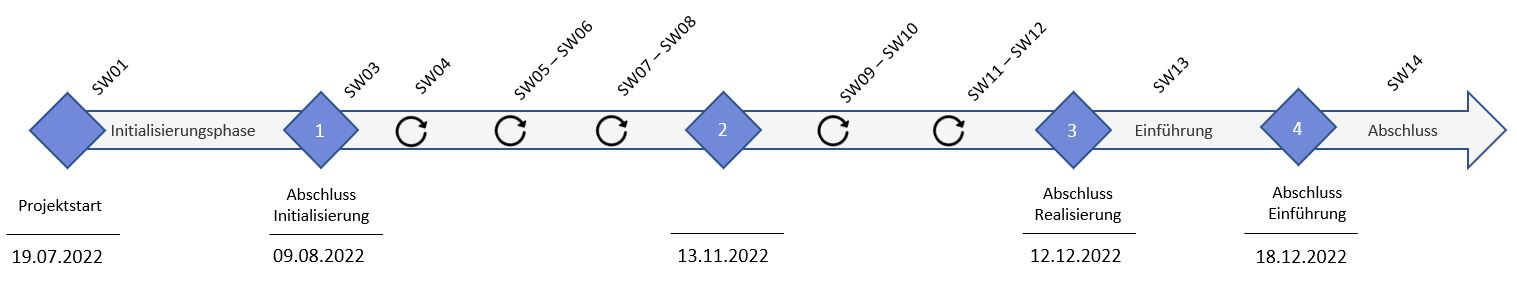
\includegraphics[width=1.3\textwidth]{img/Rahmenplan.jpg}
    \caption{Rahmenplan}
    \label{fig:Rahmenplan}
\end{figure}

Es wird entschieden, eine Initialisierungsphase von 3 Wochen zu planen, die Analyse der bestehenden Software findet in dieser Phase statt. 
Es bleibt noch eine Woche für die Einführungsphase und das Erstellen der Anleitung. 
Für die Realisierungsphase bleiben 9 Wochen, die in Sprints eingeteilt werden können. 
Zum Schluss verbleiben ein einwöchiger Sprint und 4 reguläre zweiwöchige Sprints.

\newpage
\subsubsection*{Meilensteine}
Meilensteine erlauben es, den Projektfortschritt festzustellen, in dem zuvor definierte Projektergebnisse (Artefakte) an einem gewissen Datum vorliegen.\\
Artefakte sind konkrete Dokumente oder Software, die vorliegen müssen. Zum Beispiel:
\begin{itemize}
    \item Testprotokolle
    \item Prototypen
    \item Software Releases
    \item Sprint-Planungen
    \item etc.
\end{itemize}

In \gls{SoDa} ist es normal, bei jedem Phasenwechsel einen Meilenstein zu definieren und in der Mitte der Realisierungsphase ebenfalls einen. \autocite{jenny_projektmanagement_2016} % PMB Projektplanung p23-25
Durch dieses Vorgehen erhält man 5 Meilensteine für dieses Projekt.

\begin{table}[h]
    \centering
    \begin{tabular}{|l|l|l|}
        \hline
        \rowcolor[gray]{.9} MS & Datum & Artefakte \\
        \hline
        1 & 19.09.2022 & \tabitem Aufgabenstellung \\
        \hline
        2 & 09.10.2022 & \tabitem Architekturdokument \\
         & & \tabitem Analyse \\
         & & \tabitem Testkonzept \\
         & & \tabitem Sprint-Planung 1 \\
        \hline
        3 & 13.11.2022 & \tabitem Software-Release 0.5 \\
         & & \tabitem Sprint-Planung 4 \\
        \hline
        4 & 12.12.2022 & \tabitem Software-Release 1.0 \\
         & & \tabitem Dokumentation Realisierung \\
        \hline
        5 & 18.12.2022 & \tabitem Bedienungsanleitung \\
        \hline
    \end{tabular}
    \caption{Meilensteine}
    \label{tab: Meilensteine}
\end{table}

\clearpage
\subsection{Risikomanagement}
Das Ziel jedes Projektes ist, eine möglichst hohe Wertschöpfung zu generieren. 
Doch Wertschöpfung und Risiko stehen komplementär zueinander. 
Das bedeutet, je höher die Wertschöpfung, desto höher das Risiko. 
Um die Wertschöpfung möglichst hoch zu halten und die Risiken zu minimieren, wird Risikomanagement betrieben. 
Im Risikomanagement unterscheidet man zwischen \textbf{Produktrisiken} und \textbf{Projektrisiken}. \autocite[p.~8-16]{peter_sollberger_risikomanagement_2021}
Produktrisiken werden direkt als Arbeitspakete im Projekt verbaut. 
Dabei wird geschaut, welche Gefahren für Mensch und Umwelt während der ganzen Umsetzung undwährend des Betriebs auftreten können.
Die Projektrisiken werden im Projektmanagement behandelt. 
Dabei wird geschaut, welche Probleme einen daran hindern könnten, ein Projekt erfolgreich abzuschliessen. \\
Dies könnten sein:
\begin{itemize}
    \item technische Risiken
    \item Implementierungsrisiken
    \item wirtschaftliche, industrielle und Geschäftsrisiken
\end{itemize}
\noindent
Das Ziel des Risikomanagements ist es, Risiken frühzeitig zu erkennen und entsprechende Massnahmen zu ergreifen. 
Der Prozess dabei ist folgender:
\begin{enumerate}
    \item Identifizieren
    \item Analysieren
    \item Priorisieren
    \item Massnahmen erarbeiten
    \item Überwachen
\end{enumerate}
In diesem Kapitel werden verschiedene Grundrisiken identifiziert, die während dem Projekt auftreten könnten. 
Da dieses Projekt während der Umsetzungsphase iterativ läuft, kann bei den \nameref{Sprintreviews}, ein Risiko-Update durchgeführt werden.\\\\

\begin{tabular}[h]{ll}
    \textbf{Eintrittswahrscheinlichkeit} & \textbf{Schadensausmass} \\
    \tabitem Unwahrscheinlich (1) & \tabitem Gering (1) \\
    \tabitem Möglich (2) & \tabitem Mittel (2) \\
    \tabitem Wahrscheinlich (3) & \tabitem Hoch (3) \\
    \tabitem Sehr wahrscheinlich (4) & \tabitem Kritisch (4) \\
\end{tabular}
\clearpage

\begin{longtable}[ht]{|p{1em}|p{8em}|p{10em}|p{7em}|p{5em}|p{1em}|}
    \hline
    \rowcolor[gray]{.9} \rot{ID} & \rot{Risiko} & \rot{Beschreibung} & \rot{\shortstack[l]{Eintritts-\\Wahrscheinlichkeit}} & \rot{Schadensausmass} & \rot{Risikoskala} \\*
    \hline
    R1 & Verbindung zwischen Bot und Discord bricht ab. &
    Die Verbindung zwischen dem Server (Discord) und dem Client (Bot) ist nicht mehr gewährleistet.
    Dies tritt ein, wenn der Bot keine Verbindung zum Internet mehr hat. Dadurch können keine Daten und Befehle ausgetauscht werden. &
    Wahrscheinlich & Hoch & 9 \\
    \hline
    R2 & Das Einlesen der Listen zerstört die Datenbank & Die Studenten- oder Modulliste, welche in das System eingelesen wird,
    enthält irgendwelche Escape-Characters.
    Dadurch könnte es beim Eintragen in die Datenbank zu Problemen kommen und diese im schlimmsten Fall zerstören. &
    Unwahrscheinlich & Kritisch & 4 \\
    \hline
    R3 & Discord Bot kann die vielen Benutzer/Nachrichten nicht bewältigen & Der Discord Bot kann die
    vielen einkommenden Nachrichten nicht bewältigen. Dies führt zu langen Antwortzeiten oder Fehlermeldungen beim Bot. &
    Möglich & Hoch &  6 \\
    \hline
    R4 & Berechtigungen für den Bot werden zu offen gesetzt. & Beim Erstellen des Bots oder beim Abfangen der Nachrichten werden
    die Berechtigungen für den Discord Bot zu offen gesetzt. Dies erlaubt es im, allenfalls unerwünschte Aktionen auf 
    dem Server auszuführen. &
    Wahrscheinlich & Hoch & 9 \\
    \hline
    \caption{Risiken Beschreibung}
    \label{tab: risk-description}
\end{longtable}

\clearpage
\subsubsection{Massnahmen}
Nun werden die Risiken analysiert und entsprechende Massnahmen erarbeitet.
Dabei wird das neue Risiko mit angepasster Eintrittswahrscheinlichkeit und Schadensausmass festgehalten.

\begin{longtable}[h]{|p{1em}|p{8em}|p{10em}|p{7em}|p{5em}|p{2em}|}
    \hline
    \rowcolor[gray]{.9} \rot{ID} & \rot{Risiko} & \rot{Massnahmen} &
    \rot{\shortstack[l]{Eintritts-\\Wahrscheinlichkeit\\(neu)}} &
    \rot{\shortstack[l]{Schadensausmass\\(neu)}} &
    \rot{\shortstack[l]{Risikoskala\\(neu)}} \\
    \hline
    R1 & Verbindung zwischen Bot und Discord bricht ab. & Bei Verbindungsabbrüchen oder sonstigen Fehlermeldungen wird eine
    Nachricht an den Administrator des Discord Bots gesendet. Dieser kann sich dann direkt dem Problem annehmen.
    Weiter wird automatisch ein Neuverbindungsversuch gestartet. &
    Möglich & Mittel & 4 \\
    \hline
    R2 & Das Einlesen der Listen zerstört die Datenbank & Die \gls{CSV} Datei durchläuft vor dem Einlesen verschiedene Tests, bevor sie
    in das System gespeist wird. So können unerwartete Charaktere direkt markiert und ausgeschlossen werden. &
    Unwahrscheinlich & Mittel & 2 \\
    \hline
    R3 & Discord Bot kann die vielen Benutzer/Nachrichten nicht bewältigen & Der Discord Bot muss vor dem Einsetzten in das 
    produktive System auf Client Auslastung getestet werden. So können unangenehme Überraschungen verhindert werden. &
    Unwahrscheinlich & Mittel &  2 \\
    \hline
    R4 & Berechtigungen für den Bot werden zu offen gesetzt. & Beim Erstellen des Bots oder beim Abfangen der Nachrichten werden alle 
    Berechtigungen am Anfang deaktiviert. Per Ausschlussverfahren werden Sie wieder aktiviert. So wird gewährleistet, dass nur benötigte
    Berechtigungen gesetzt sind. &
    Unwahrscheinlich & Gering & 1 \\
    \hline
    \caption{Risiken Massnahmen}
    \label{tab: risk-measures}
\end{longtable}

\subsubsection{Risikomatrix}
Die Risiken werden in eine sogenannte Risikomatrix eingetragen, wobei die Achsen die Eintrittswahrscheinlichkeit und das Schadensausmass darstellen. 
In dieser Matrix kann die Risikobereitschaft der Projektverantwortlichen eingetragen werden. 
Die Risikobereitschaft wird mit einer Linie durch die Matrix dargestellt. 
In dem Projekt wäre es der orangene und rote Bereich, welcher über der Bereitschaftslinie liegt. 
Wenn ein Risiko über der Linie liegt, müssen zwingend andere Massnahmen ergriffen werden.\\
Das Ziel ist es mit den getroffenen Massnahmen alle Risiken unter diese Risikobereitschaftslinie zu bringen.

\begin{table}[h]
    \centering
    \begin{tabular}{|l|p{2cm}|p{2cm}|p{2cm}|p{2cm}|}
        \hline
        \shortstack[c]{Schadensausmass / \\ Eintrittswahrscheinlichkeit} & Gering & Mittel & Hoch & Kritisch \\[10pt]
        \hline
        Sehr wahrscheinlich & \cellcolor{yellow!50} & \cellcolor{orange!50} & \cellcolor{red!50} & \cellcolor{red!50} \\[10pt]
        \hline
        Wahrscheinlich & \cellcolor{yellow!50} & \cellcolor{yellow!50}& \cellcolor{orange!50}(R1, R2) & \cellcolor{red!50} \\[10pt]
        \hline
        Möglich & \cellcolor{green!50} & \cellcolor{yellow!50}R1 & \cellcolor{yellow!50}(R3, R4) & \cellcolor{orange!50} \\[10pt]
        \hline
        Unwahrscheinlich & \cellcolor{green!50}R4 & \cellcolor{green!50}R2, R3 & \cellcolor{yellow!50} & \cellcolor{yellow!50} \\[10pt]
        \hline
    \end{tabular}
    \caption{Risikomatrix}
    \label{tab: Riskmatrix}
\end{table}

\clearpage
\section{Realisierung}\label{implementation}

\subsection{Analyse der bestehenden Infrastruktur}
Als erster Schritt wird eine Analyse des bestehenden Bots und seiner Funktion im Discord durchgeführt.

\subsubsection{Aufbau Discord}
Der Discord Server "STAIR" wird von STAIR verwaltet und ist ein online Treffpunkt für alle Studierenden des Departments Informatik. 
Beim erstmaligen Eintreten in den Server hat man noch keine Berechtigungen. 
Es wird deshalb ausser dem Help Channel noch nichts angezeigt. 
Man bekommt vom Bot Stan, nach Eintreten in den Server, eine Nachricht mit einer Anleitung. 
Darin ist beschrieben, wie man sich authentifiziert. 
Bei der Authentifizierung wird vom Bot geschaut, ob es sich um eine Studierenden E-Mailadresse handelt. 
Wenn dem so ist, schickt der Bot einen 6-stelligen Random Code, den der Benutzer im Discord dem Bot zurückschreiben muss.\\
Hat dieser Prozess funktioniert, ist man "eingeloggt" und bekommt vom Bot die Rolle Student/in zugeteilt. 
Damit hat man Zugriff auf die verschiedenen Grund-Channels, wie Gaming, Administration, General, Studying, etc.. 
In diesen Channels können sich Studierende mit anderen Studierenden sprachlich oder per Text über Themen austauschen.\\\\
Der STAIR Discord-Server bietet auch Informationen und Unterstützung für alle Module an. 
Dabei hat jedes Modul einen eigenen Channel. 
Dort können sich Studierende gezielt über ein Modul austauschen, Fragen stellen oder Informationen mitteilen. 
Für diese Module muss man sich spezifisch registrieren, erst danach werden diese angezeigt. 
So wird verhindert,
\begin{enumerate}
    \item dass man unn\"otig Benachrichtigungen von Channels bekommt, die einen nicht interessieren.
    \item dass sein Discord nicht \"uberf\"ullt wird mit ca. 530 Modul-Channels.
\end{enumerate}
Die Commands \textit{show <module>} und \textit{hide <module>} erlauben es, den Channel hinzuzuf\"ugen oder zu entfernen.
Bei der derzeitigen Version des Discord Bots wird die Anzahl Rollen, die vergeben werden können, zum Problem. 
(Siehe Kapitel \ref{discord_einschraenkungen})
Durch eine Anzahl von etwa 350 Modulen, welche am Departement Informatik unterrichtet werden, kann die Modulfreigabe nicht mit Rollen gelöst werden. 
Zum jetzigen Zeitpunkt werden die Module in einzelnen Themenbereichen zusammengefasst. 
Beispielsweise alle Security Module in einer Kategorie. 
Bei einem Show-Command wird den Studierenden nun die Rolle der entsprechenden Kategorie zugeteilt. 
Mit diesem Vorgang erhält der Studierende aber Einsicht in alle Module dieser Kategorie, was vielleicht gar nicht erwünscht ist.\\\\
Neu gibt es das Konzept der verschiedenen Häuser bei STAIR. 
Jeder Studierende wird dabei einem Haus zugeteilt. 
Die Zuteilung läuft dabei über das Sekretariat der Hochschule. 
Es wird geschaut, dass in jedem Studiengang, in jedem Startsemester die Studierenden gleichmässig auf die Häuser verteilt werden. 
Es gibt die Häuser Blue, Purple, Red, Orange, Yellow und Grey. 
Während dem Semester organisiert STAIR verschiedene Events, bei denen Punkte für sein Haus gesammelt werden können. 
Am Ende jedes Studienjahres wird das Haus, welches am meisten Punkte gesammelt hat, als Gewinner gelobt.\\
Der Discord-Server bietet die Plattform, um sein Haus zu mobilisieren oder die neuesten Ergebnisse den Studierenden zu verkünden. 
Pro Haus gibt es einen Channel. Momentan werden die Studierenden noch manuell zu ihren zugehörigen Channels hinzugefügt.
In der folgenden Abbildung sieht man eine Übersicht über alle Discord Channels und Kategorien, wie sie momentan bestehen.

\begin{figure}[h]
    \centering
    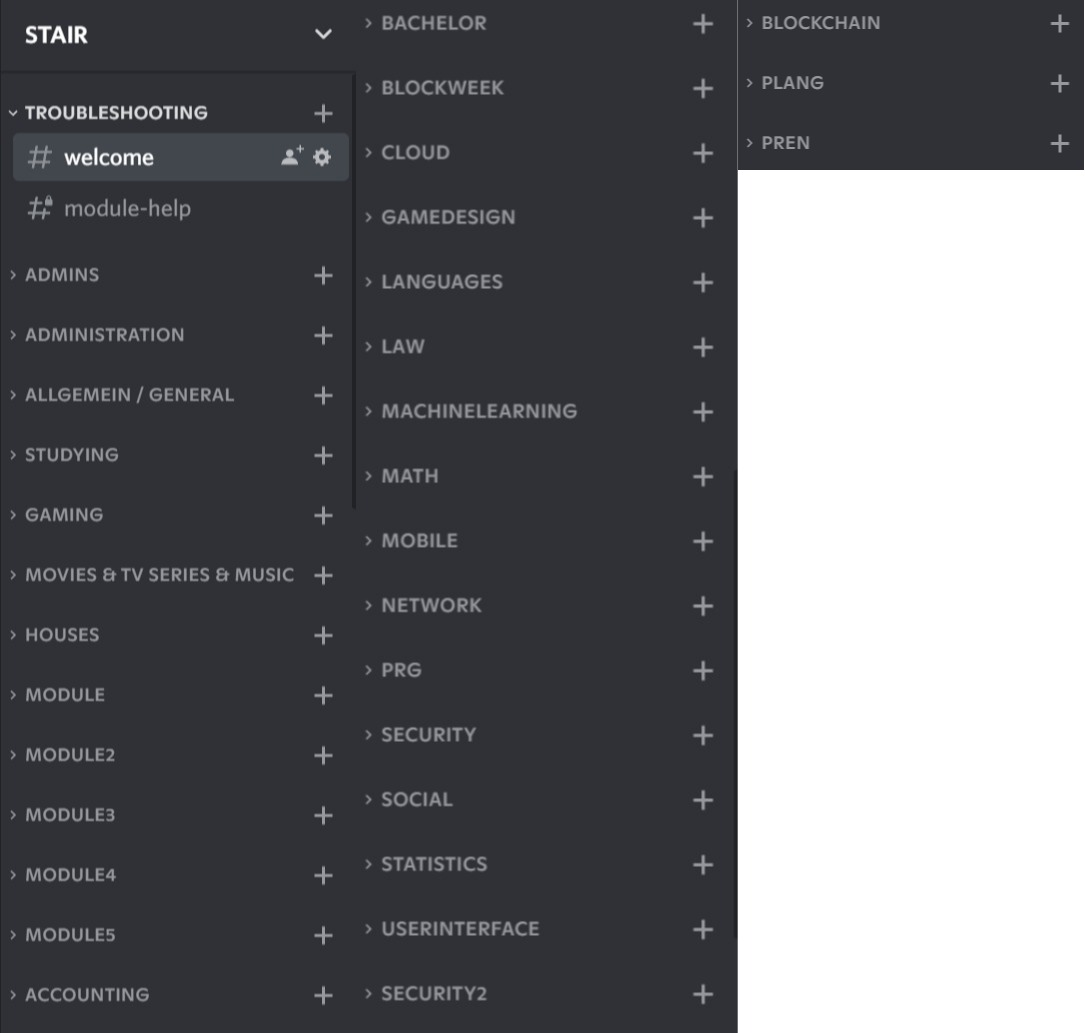
\includegraphics[width=1.0\textwidth,height=10cm]{img/Stair_Discord_Channels.jpg}
    \caption{STAIR Discord Channels Alt}
    \label{fig:stair_old_discord_channels}
\end{figure}

\subsubsection*{Ablauf Authentifizierung \& Modulanmeldung}
In den folgenden zwei Seiten werden der Authentifizierungsprozess und der Modulanmeldungsprozess als Ablaufdiagramm beschrieben. 
Dieser Ablauf wird zum jetzigen Zeitpunkt durchgeführt.

\begin{landscape}
    \begin{figure}[ht]
        \centering
        \hspace*{-4.1cm}
        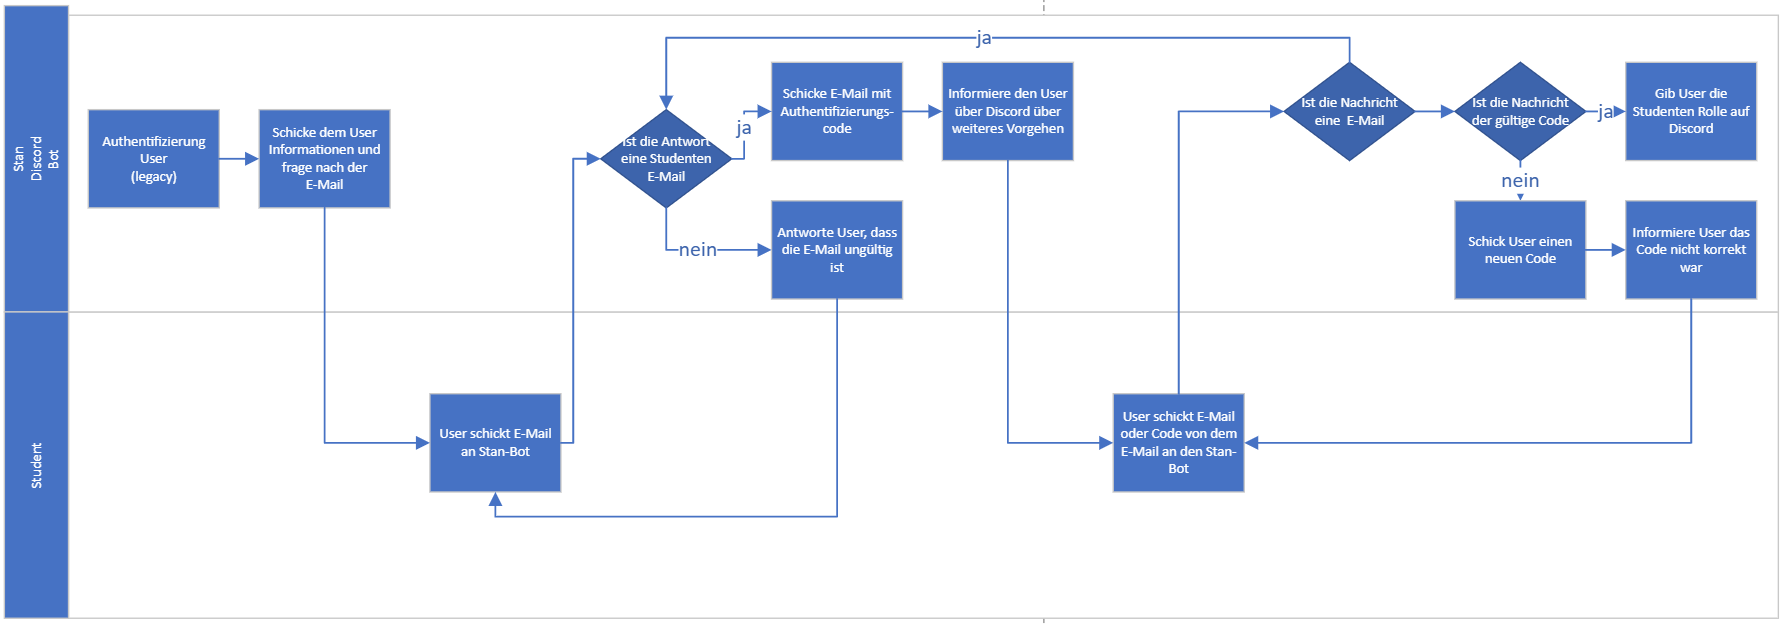
\includegraphics[width=1.9\textwidth]{img/Authentifizierungsprozess_Bot_alt.png}
        \caption{Authentifizierungsprozess Bot alt}
        \label{fig:Authentifizierungsprozess_Bot_alt}
    \end{figure}
    \clearpage
    \begin{figure}[ht]
        \centering
        \hspace*{-4.1cm}
        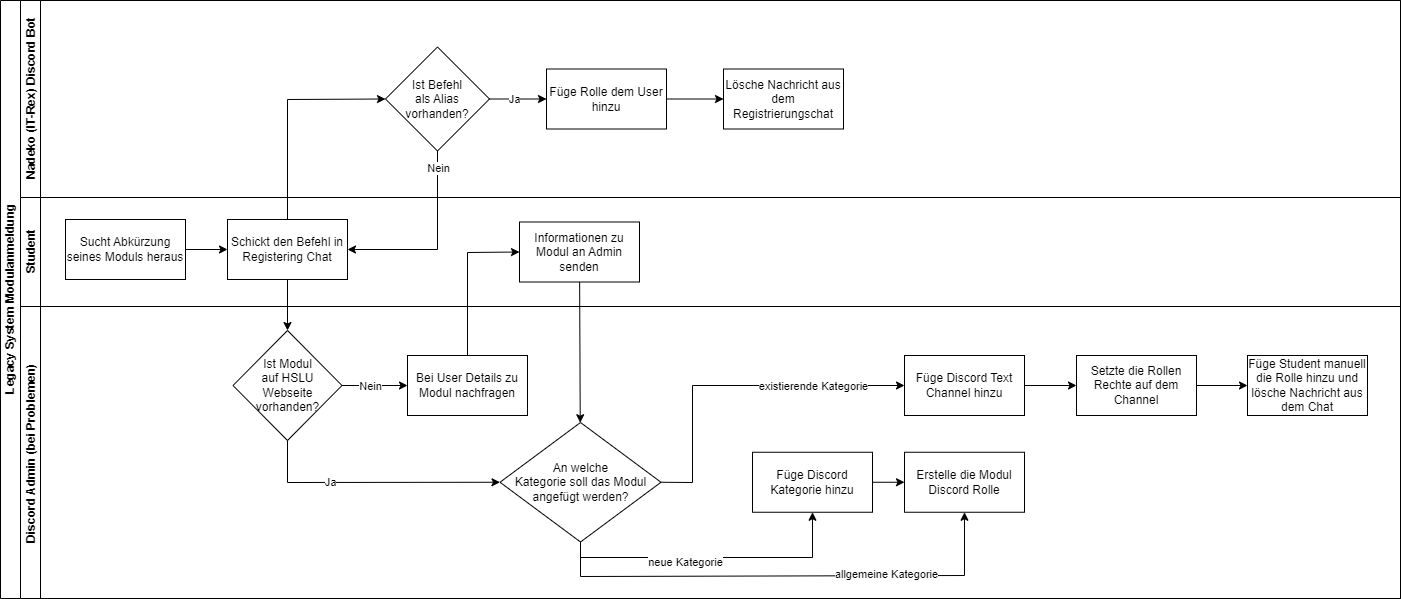
\includegraphics[width=1.9\textwidth]{img/Modulanmeldungsprozess_Bot_alt.png}
        \caption{Modulanmeldungsprozess Bot alt}
        \label{fig:Modulanmeldungsprozess_Bot_alt}
    \end{figure}
\end{landscape}

\subsubsection{Funktionsweise Bot}
Der Bot ist mit der Programmiersprache C\# und dem .NET Framework geschrieben.

\subsubsection*{Konfigurationsmanagement alter Bot}
In der folgenden Tabelle ist eine Übersicht der verwendeten IDE, ihrer Spezifizierung und den eingesetzten Libraries.

\begin{table}[h]
    \centering
    \begin{tabular}{|l|p{20em}|l|}
        \hline
        \rowcolor[gray]{.9} Name & Beschreibung & Version \\
        \hline
        .NETCore & Core Library für C\# Projekte.
        Enthält alle grundlegend Klassen und Libraries, welche für die Erstellung von .NET Projekten nötig sind. & 2.0.0 \\
        \hline
        NETStandard Library & Set von Standard .NET \gls{API}s & 2.0.3 \\
        \hline
        Discord.NET & Asynchrone \gls{API} für Discord. & 2.3.0 \\
        \hline
        FakeItEasy & Mocking Bibliothek & 6.0.0 \\
        \hline
        FluentAssertions & Spezifizieren von TDD und BDD-Style Unit Tests. & 5.10.2 \\
        \hline
        Microsoft UserSecrets & User Secret Konfigurations provider & 3.1.0 \\
        \hline
        Microsoft Graph & Erlaubt alle Microsoft Dienste über eine einheitliche Schnittstelle anzusprechen & 1.21.0 \\
        \hline
        Microsoft.Identity.Client & Enthält Binaries für die Microsoft Authentication Library (MSAL) & 4.7.1 \\
        \hline
        Newtonsoft.JSON & High-Performance Framework für \gls{JSON} & 12.0.3 \\
        \hline
        Ninject & Dependency Injector für .NET Applikationen & 3.3.4 \\
        \hline
        Nito.AsyncEx & Hilfsbibliothek für Task-Based Asynchronous Pattern (TAP) & 5.0.0 \\
        \hline
        Topshelf & Bibliothek zum Hosten von Applikationen. 
        Bietet command-line Optionen zum Installieren, konfigurieren und laufen lassen von applications as a service. & 4.2.1 \\
        \hline
        xunit & Developer testing framework & 2.4.1 \\
        \hline
    \end{tabular}
    \caption{Konfigurationsmanagement Bot alt}
    \label{tab: Konfigurationsmanagement-Bot-alt}
\end{table}

Das Programm, welches den Bot zur Verfügung stellt, ist nicht gross. 
Beinhaltet im Groben einen Client Socket, der Events on Discord abfängt und einer E-Mail Klasse, die E-Mails an den Benutzer versenden kann. 
Das Programm ist in zwei Packages aufgeteilt:
\begin{itemize}
    \item StanBot.Core
    \item StanBot.Service
\end{itemize}
Eine grosse Version des Diagramms findet man im Anhang im Kapitel \nameref{diagrams}.
\clearpage

\begin{figure}[ht]
    \centering
    \hspace*{-1.5cm}
    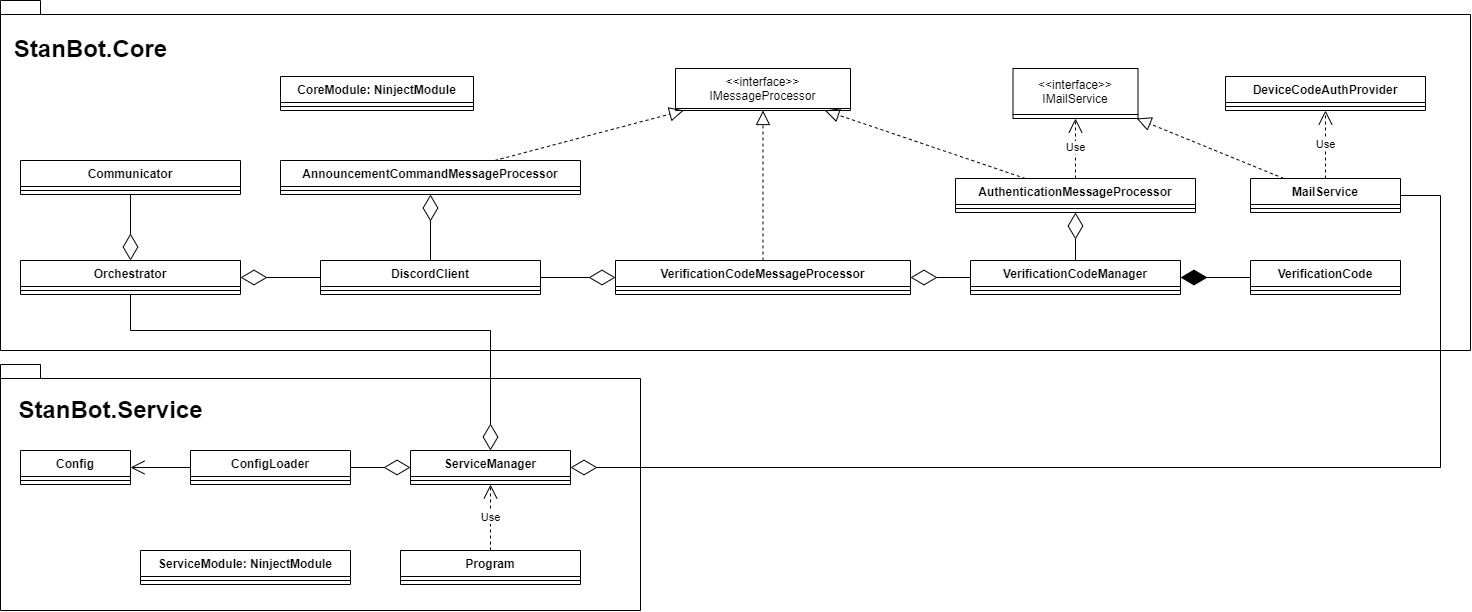
\includegraphics[width=1.2\textwidth]{img/Klassendiagramm_Bot_alt.png}
    \caption{Klassendiagramm Bot alt}
    \label{fig:Klassendiagramm_Bot_alt}
\end{figure}

\subsubsection{Ausführung Bot}
Der Bot läuft auf einem Microsoft Windows Server 2019 Standard auf der Enterprise Lab Umgebung der HSLU. 
Die Konfiguration entspricht der eines Windows Services und läuft dementsprechend durchgehend.

\begin{figure}[hb]
    \centering
    \hspace*{-2.5cm}
    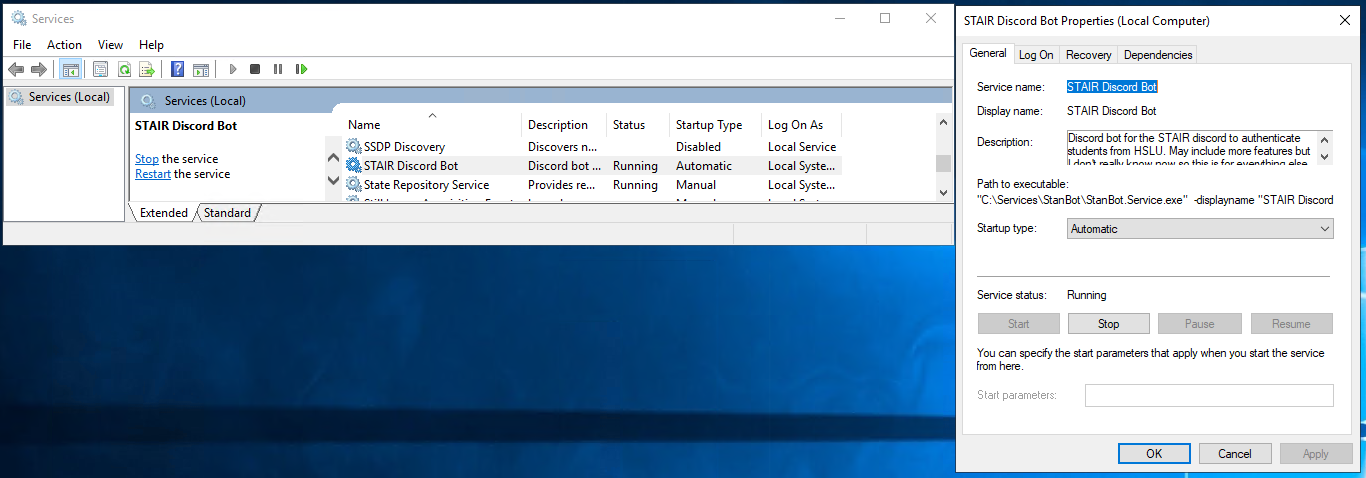
\includegraphics[width=1.3\textwidth,height=6cm]{img/Discord_Bot_old_service_configuration.png}
    \caption{Stair Discord Service Konfiguration Alt}
    \label{fig:bot-service-configuration-old}
\end{figure}
\clearpage

\subsubsection{Geplante Änderungen}\label{geplanteAenderungen}

\subsubsection*{Wechsel zu Linux Server}
Es wird zusammen mit dem STAIR Team entschieden, auf Linux zu wechseln, um alle Server einheitlich auf Linux zu haben. 
Bei STAIR wird noch eine Wordpress-Seite und eine JavaScript Webseite betrieben. 
WordPress ist ein Content Management System (CMS) und wird bei STAIR eingesetzt für die Hauptwebseite, auf der alle Events und weitere Informationen ersichtlich sind. 
Da die Projekte sich stark voneinander unterscheiden, wird entschieden, mit verschiedenen Servern zu arbeiten und nicht alle auf dem gleichen Server zu hosten. 
Gleichzeitig befindet sich die WordPress-Seite noch auf einem anderen Rechencenter als dem Enterprise Lab der HSLU. 
Dies verursacht Kosten, die eingespart werden sollen in Zukunft. 
Um den Transfer zu vereinfachen, macht es Sinn, nicht einen ohnehin bald obsoleten Server für das Deployment zu nutzen.

\subsubsection*{Entscheid den Bot neu zu schreiben}
Bei der Analyse des bisherigen Bot wird bemerkt, dass die veraltete Technologie .NET Standard 2.0 und .NET Core 3.1 mit veralteten Libraries genutzt wird. 
Diese werden nicht mehr unterstützt und sollten ersetzt werden. 
Für die neue Version wird .NET 6 mit C\# verwendet. 
Dies ermöglicht es, Inspiration bei der alten Lösung zu holen, falls zum Beispiel die Verwendung der Discord Library unklar ist oder bei einem bereits existierenden Feature ein Problem auftaucht. 
Die neueren .NET Versionen sind Cross-Plattform fähig und können auf Linux verwendet werden.\autocite{de_george_installieren_nodate}
Die Sprache wird an der Hochschule nicht breit verwendet, es gibt jedoch das Modul \textit{C\# in Action}\autocite{noauthor_bachelor_nodate}, wo die Sprache erklärt wird und die Sprache ist ohnehin ähnlich zu Java, welche grundsätzlich an der Hochschule unterrichtet wird.
Das WIPRO Team ist zusätzlich bereits vertraut mit C\# als Sprache und hat diese als angenehm empfunden, was die Entscheidung zusätzlich unterstützte. 

\subsubsection*{Entscheid Login Funktionsweise}

Beim Login wird überlegt, das Switch-Login der Hochschule zu verwenden, welches auch für aussenstehende Zwecke verwendet werden kann. 
Es wird dagegen entschieden, da STAIR nicht die volle Kontrolle über den Service hat. 
Es können plötzlich neue Interface Standards erlassen werden, was zu Problemen führen kann. 
Es muss hierzu ein bestimmter Link geöffnet werden, welcher von Stan verschickt werden muss, um die Switch Login Seite zu öffnen. 
Dies könnte nicht vertrauenswürdig wirken bei Studierenden. 
Ausserdem hat sich das Login mittels E-Mails bereits bewährt, weshalb dieses nun weiterhin verwendet wird.

%\subsubsection*{Wechsel zu Community Server}
% https://support.discord.com/hc/en-us/articles/360047132851-Enabling-Your-Community-Server

\subsubsection*{Entscheid zur Anbindung an eine Datenbank}
Eine Datenbank bringt einige Vorteile. 
Speziell relevant sind folgende Punkte für dieses Projekt:
\begin{itemize}
    \item Eine Datenbank ermöglicht eine automatische Zuweisung von Studierenden zu ihren Häusern.
    \item Sie ermöglicht das automatische markieren von Exstudierenden.
    \item Sie bietet die grösste Erweiterbarkeit für die Zukunft.
    \item Modul-Channels, welche zur Zeit nicht gebraucht werden, könnten theoretisch auf Discord gelöscht werden. Bei Bedarf können die Modul-Channels wieder neu erstellt werden.
    \item Bei Problemen kann schnell herausgefunden werden, welche Person betroffen ist und man kann die Person über alternative Kommunikationswege, wie E-Mail, kontaktieren.
    \item Studierende können über ihre E-Mail permanent gebannt werden, ohne dass sie sich mit neuen Discord Accounts wieder anmelden können.
\end{itemize}
Eine Datei wäre ebenfalls möglich zur Datenspeicherung. 
Diese hätte jedoch weniger Performance und würde keine Checks durchführen beim Speichern der Daten. 
Das Auslesen von gefilterten Daten gestaltet sich ebenfalls einfacher.\autocite{castro_why_2020}
Da es bei diesem Projekt wichtig ist, dass die Daten korrekt im Schema gespeichert werden wurde eine SQL basierte Datenbank bevorzugt gegenüber von NoSQL Datenbanken. 
Als gewählte Technologie hat sich MySQL durch seine grosse Verbreitung sehr gut angeboten. 
Online wird MySQL als die zweitmeist genutzte Datenbank-Technologie beschrieben.\autocite{noauthor_db-engines_2022}

\subsubsection*{Entscheidung einen eigenen Bot zu entwickeln}
Zusammen mit STAIR wurde entschieden, wieder eine eigens entwickelte Lösung zu wählen. 
Dies hat verschiedene Vorteile. 
Als erstes ist damit gleich auch der Datenschutz gewährleistet. 
Auch sind so keine künstlichen Limitierungen eines extern entwickelten Bots vorhanden. 
Die einzigen Limitierungen sind vom \gls{API} von Discord und von technischen Know-How der betreuenden Entwicklern. 
Da die verschiedenen Bots eventuell nicht in Europa gehostet sind, könnten Verbindungs- und/oder Performanceprobleme auftreten. 
Durch die Log Datei(en) können Fehler einfacher gefunden und nachvollzogen werden.

\newpage
\subsection{Initialisierungsphase}
Aus dem Projektauftrag und aus den Wünschen der Stakeholder werden Anforderungen an das Produkt definiert. 
Diese werden für die Realisierungsphase in Epics umgewandelt. 
Die Epics werden im Anschluss in einzelne User Stories aufgeteilt, die dann in den Sprints separat behandelt und gelöst werden.

\subsubsection{Epics}\label{Epics}
Für das Projekt werden folgende Epics definiert.

\begin{table}[h]
    \centering
    \begin{tabular}{ | p{1em} | p{35em} | p{2em} |}
        \hline
        \rowcolor[gray]{.9} ID & Beschreibung & Prio \\
        \hline
        1 & Der Nutzer wird beim erstmaligen Betreten des Discord-Servers vom Bot benachrichtigt.
        Dieser gibt ihm Grundlegende Informationen zum Server und dem Authentisierungsprozess.
        Zu diesem Zeitpunkt hat der Student noch keine Berechtigungen auf dem Server und
        hat nur Zugriff auf den Channel "Help". & A \\
        \hline
        2 & Der Bot soll den Nutzer authentifizieren und mit der Studenten-Rolle versehen können.
        Er kann dabei zwischen den E-Mails von Nicht-Student und Student unterscheiden und auf unvorhergesehene
        Interaktionen, von Seiten des Benutzers, reagieren können. & A \\
        \hline
        3 & Ein Student kann sich beim Bot für ein Modul anmelden. Dieser schaltet den Channel für den Studenten frei,
        so das er darin mit anderen Studierenden kommunizieren kann. Falls das Modul für den Studenten nicht mehr relevant ist,
        kann er es beim Bot wieder abmelden. & A \\
        \hline
        4 & Die Administration des Discord Servers soll einfach neue Modullisten in das System laden können.
        Die neuen oder nicht mehr Verfügbaren Module werden erkannt und entsprechend hinzugefügt oder gelöscht.
        An dem Verhalten des Benutzers soll sich nichts ändern. & A \\
        \hline
        5 & Die Administration kann jedes Semester die neuen Studierenden hinzufügen.
        Diese werden beim potentiellen Authentifizieren direkt in Ihre zugeteilten Häuser-Channels zugewiesen. & A \\
        \hline
        6 & Die Administration von STAIR kann über eine zur Verfügung gestellte Schnittstelle, Statistiken über
        den Discord erstellen. & B \\
        \hline
        7 & Fehlereingaben in dem Modul-Registrierungs-Channel oder interne Fehler vom Bot, sollen direkt automatisch
        an einen hinterlegten Mitarbeiter von STAIR gemeldet werden & C \\
        \hline
    \end{tabular}
    \caption{Epics}
    \label{tab: Epics}
\end{table}

\subsubsection{User Stories}\label{user-stories}
Die Epics werden in kleinere User-Stories heruntergebrochen und dienen als Bausteine eines Sprints.
Dieser Prozess wird auch \textbf{Story-Splitting} genannt
User-Stories sind immer nach dem gleichen Muster aufgebaut. \\
"Als <Rolle> möchte ich <Ziel/Wunsch>, um <Nutzen>." \\
Die Story muss nicht immer aus der Benutzersicht definiert sein, sondern es können auch technische oder infrastrukturelle User-Stories so gebildet werden.\\
In der Sprint-Planung werden zu jeder User-Story zugehörige Akzeptanzkriterien definiert. 
Diese dienen zur Kontrolle, ob die User-Story korrekt umgesetzt wurde und können auch als Test während der Entwicklung gebraucht werden. 
Später können dann die Mitglieder des Teams den Aufwand der Story realistisch abschätzen.\\
Gute User-Stories können nach dem Modell \textbf{I.N.V.E.S.T} gebildet werden. \autocite{hammerschall_software_2013} % PMB Projektplanung p.101-103
\begin{itemize}
    \item \textbf{I}ndependent  unabhängig voneinander
    \item \textbf{N}egotiable   zerlegbar, änderbar, kombinierbar, verhandelbar
    \item \textbf{V}aluable     hat wirtschaftlichen Wert
    \item \textbf{E}stimatable  so klar, dass es vom Team geschätzt werden kann
    \item \textbf{S}mall        klein genug, um in einem Sprint entwickelt werden zu können
    \item \textbf{T}estable     klare Akzeptanzkriterien
\end{itemize}
Beim Story-Splitting werden folgende User-Stories für das Projekt definiert.

\begin{longtable}{ | p{1em} | p{16em} | p{13em} | p{2em} | p{3em} | p{2em} |}
    \hline
    \rowcolor[gray]{.9} ID & Beschreibung & Akzeptanzkriterien & Prio & Weight & Sprint \\
    \hline
    1 & Als Bot möchte ich den Benutzer beim ersten Betreten des Server authentifizieren können,
    um ihm die ihm zugeteilten Rollen zuweisen zu können. &
    \tabitem Der Nutzer bekommt beim ersten Betreten des Servers eine Nachricht vom Bot mit Informationen. & A & 12 & 2 \\*
    & & \tabitem Der Student bekommt nach der Anmeldung die Rolle Student zugeteilt und wird dem richtigen Haus-Channel zugewiesen. & & & \\
    \hline
    2 & Als Bot möchte ich den Studenten mittels E-Mail Verifikation authentifizieren können,
    um sicher zu gehen, dass dieser eine gültige Studenten-Mail besitzt. &
    \tabitem Der Student bekommt eine E-Mail auf der Adresse, die er dem Bot mitteilt. & A & 15 & 3 \\*
     & & \tabitem Ein Student kann sich authentifizieren, ein Nicht-Student wird abgewiesen. & & & \\*
     & & \tabitem In der E-Mail steht ein zufällig generierter 6-stelliger Code. & & & \\*
     & & \tabitem Der Bot kann den Code verifizieren, nachdem der Student die E-Mail erhalten hat. & & & \\
    \hline
    3 & Als STAIR Administrator möchte ich neue Studenten einfach erfassen können,
    um sie dem System bekannt zu machen und die Administration zu vereinfachen. &
    \tabitem Neue Studenten können mit ihren zugeteilten Häusern als Liste eingelesen werden & B & 9 & 1 \\*
     & & \tabitem Die neu erfassten Studenten werden im System eingetragen und können für die Authentifizierung verwendet werden. & & & \\
    \hline
    4 & Als Student möchte ich mich für neue Modul-Channels an und abmelden können,
    um mich mit anderen Studenten austauschen zu können. &
    \tabitem Es stehen Befehle im \textbf{Registrierungs-Channel} zur Verfügung, um sich bei Modulen an- und abzumelden. & A & 12 & 3 \\*
     & & \tabitem Der Bot weist den Studenten, bei einer Anmeldung, dem Modul als Mitglied hinzu. & & & \\*
     & & \tabitem Der Bot löscht den Studenten, bei einer Abmeldung, aus der Mitgliederliste,
     so dass der Channel für den Studenten nicht mehr sichtbar ist. & & & \\
    \hline
    5 & Als STAIR Administrator möchte ich Modullisten mit den verfügbaren Modulen, einfach in das System eintragen zu können,
    um sie für den Bot nutzbar zu machen. &
    \tabitem Pro Semester können Modullisten automatisch eingelesen werden. & B & 8 & 2 \\*
     & & \tabitem Neue Module werden automatisch hinzugefügt, und solche, welche nicht mehr Unterrichtet werden, werden gelöscht. & & & \\*
     & & \tabitem Die Module stehen nach dem einlesen direkt bereit, zur Channel-Erstellung durch den Bot. & & & \\
    \hline
    6 & Als STAIR Administrator möchte ich Statistiken aus dem System auslesen können,
    um sie für Marketing oder andere Zwecke gebrauchen zu können. &
    \tabitem Es stehen ein paar vorgefertigte Auslesemöglichkeiten bereit, um sie für den Administrator nutzbar zu machen & C & 9 & 4 \\
    \hline
    7 & Als STAIR Administrator möchte ich sofort benachrichtigt werden, falls mit dem System etwas nicht stimmt,
    um Gegenmassnahmen ergreifen zu können. &
    \tabitem Der Administrator wird benachrichtigt, wenn der Bot zu Discord oder zur Datenbank keine Verbindung mehr hat & C & 5 & 5 \\*
     & & \tabitem Der Administrator wird benachrichtigt wenn der E-Mail Versand zur Authentifikation nicht mehr funktioniert. & & & \\
    \hline
    \caption{User-Stories}
    \label{tab: UserStories}
\end{longtable}

\subsubsection*{Sprintplanung}
\begin{table}[h]
    \centering
    \begin{tabular}{|l|l|l|l|}
        \hline
        \rowcolor[gray]{.9} Sprint & Start & Ende & Artefakte \\
        \hline
        Sprint 1 & 10.10.2022 & 16.10.2022 & \tabitem Studentenerfassung implementiert \\
         & & & \tabitem Sprintreview S01 \\
         & & & \tabitem Sprint-Planung S02 \\
        \hline
        Sprint 2 & 17.10.2022 & 30.10.2022 & \tabitem Modulerfassung implementiert \\
         & & & \tabitem Sprintreview S02 \\
         & & & \tabitem Sprint-Planung S03 \\
        \hline
        Sprint 3 & 31.10.2022 & 13.11.2022 & \tabitem Authentifizierung implementiert \\
         & & & \tabitem Sprintreview S03 \\
         & & & \tabitem Sprint-Planung S04 \\
        \hline
        Sprint 4 & 14.11.2022 & 27.11.2022 & \tabitem Statistiken implementiert \\
         & & & \tabitem Sprintreview S04 \\
         & & & \tabitem Sprint-Planung S05 \\
        \hline
        Sprint 5 & 28.11.2022 & 11.12.2022 & \tabitem Fehlererkennung implementiert \\
         & & & \tabitem Sprintreview S05 \\
        \hline
    \end{tabular}
    \caption{Sprintplanung}
    \label{tab: Sprintplanung}
\end{table}

Die Projektkontrolle und der Fortschritt wird mit folgenden Tools überwacht.
\begin{itemize}
    \item Github Story-Board (\href{https://github.com/orgs/stairch/projects/1/views/4}{Link zum Story-Board})
    \item Sprintreviews (\nameref{Sprintreviews})
\end{itemize}

\subsubsection{Testdrehbuch}\label{Testdrehbuch}
Wie im Kapitel \nameref{Teststrategie} erwähnt, werden im Folgenden die einzelnen Systemtests beschrieben.
Diese müssen alle manuell vor der Übergabe der Software durchgeführt werden.\\
Sie beziehen sich immer auf eine Anforderung / Epic und können so auch bei den einzelnen Sprintreviews zur Kontrolle verwendet werden. 
Die Referenzierten Epics sind im Kapitel \nameref{Epics} beschrieben.

\begin{longtable}[ht]{|p{15em}|p{25em}|}
    \hline
    \multicolumn{2}{|l|}{\textbf{Betritt ein neuer Student den Discord-Server, bekommt er direkt eine Nachricht.}} \\*
    \multicolumn{2}{|l|}{\textbf{vom Stan Bot.}} \\
    \hline
    \multicolumn{2}{|l|}{\textbf{Testfall \#1}} \\
    \hline
    \textbf{Epic / Anforderung} & \#1 \\
     & Der Nutzer wird beim erstmaligen Betreten des Discord-Servers vom Bot benachrichtigt.
     Dieser gibt ihm Grundlegende Informationen zum Server und dem Authentifizierungsprozess.
     Zu diesem Zeitpunkt hat der Student noch keine Berechtigungen auf dem Server und
     hat nur Zugriff auf den Channel "Help". \\
    \hline
    \textbf{Durchführung} &
    \begin{enumerate}
        \item Bereitstellen eines Discord Accounts, welcher noch nicht auf dem STAIR-Discord Server angemeldet ist.
        \item Dem STAIR Discord Server beitreten. \url{https://discord.com/invite/Tp7XgzZ}
    \end{enumerate}\\
    \hline
    \textbf{Erwartetes Ergebnis / Verhalten} & Sobald man dem Server beigetreten ist, bekommt man vom Stan Bot eine private Nachricht.
    Dort stehen allgemeine Informationen zum Server und zum Anmeldeprozess. \\
    \hline
    \caption{Testdrehbuch - Testfall \#1}
\end{longtable}

\begin{longtable}[h]{|p{15em}|p{25em}|}
    \hline
    \multicolumn{2}{|l|}{\textbf{Ein Student kann sich beim Bot authentifizieren.}} \\
    \hline
    \multicolumn{2}{|l|}{\textbf{Testfall \#2}} \\
    \hline
    \textbf{Epic / Anforderung} & \#2 \\*
     & Der Bot soll den Nutzer authentifizieren und mit der Studenten-Rolle versehen können. \\
    \hline
    \textbf{Durchführung} &
    \begin{enumerate}
        \item Der Student hat eine Nachricht von Stan als Direkt Nachricht erhalten.
        \item Der Student schickt dem Bot seine E-Mail Adresse nach dem Muster \textit{<name.vorname>@stud.hslu.ch} .
        \item Nach Erhalt der E-Mail, schickt der Student, Stan den 6-stelligen Verifizierungscode.
    \end{enumerate}\\
    \hline
    \textbf{Erwartetes Ergebnis / Verhalten} & Der Student sollte nach Senden seiner E-Mail Adresse dem Bot, eine E-Mail von ihm erhalten.
    In dieser ist ein zufällig generierter 6-stelliger Verifizierungscode enthalten.
    Nach dem verifizieren, bekommt der Nutzer die Rolle Student und "Haus" zugeteilt und hat Zugriff auf die Grund-Channels. \\
    \hline
    \caption{Testdrehbuch - Testfall \#2}
\end{longtable}

\begin{longtable}[h]{|p{15em}|p{25em}|}
    \hline
    \multicolumn{2}{|l|}{\textbf{Ein Nicht-Student kann sich nicht authentifizieren.}} \\
    \hline
    \multicolumn{2}{|l|}{\textbf{Testfall \#3}} \\
    \hline
    \textbf{Epic / Anforderung} & \#2 \\*
     & Er kann dabei zwischen den E-Mails von Nicht-Student und Student unterscheiden und
     auf unvorhergesehene Interaktionen, von Seiten des Benutzers, reagieren können. \\
    \hline
    \textbf{Durchführung} &
    \begin{enumerate}
        \item Ein Nicht-Student schickt dem Bot eine E-Mail, welche sich vom Muster \textit{<name.vorname>@stud.hslu.ch} unterscheidet.
    \end{enumerate}\\
    \hline
    \textbf{Erwartetes Ergebnis / Verhalten} & Der Nutzer bekommt direkt eine Nachricht vom Bot, das diese E-Mail nicht gültig ist.
    Es können sich nur Studenten authentifizieren. \\
    \hline
    \caption{Testdrehbuch - Testfall \#3}
\end{longtable}

\begin{longtable}[h]{|p{15em}|p{25em}|}
    \hline
    \multicolumn{2}{|l|}{\textbf{Ein STAIR Administrator kann eine Liste mit Studenten in das System einlesen.}} \\
    \hline
    \multicolumn{2}{|l|}{\textbf{Testfall \#4}} \\
    \hline
    \textbf{Epic / Anforderung} & \#5 \\*
     & Die Administration kann jedes Semester die neuen Studierenden hinzufügen.
     Diese werden beim potentiellen Authentifizieren direkt in Ihre zugeteilten Häuser-Channels zugewiesen. \\
    \hline
    \textbf{Durchführung} &
    \begin{enumerate}
        \item Der STAIR Administrator muss sich eine Liste von Studenten mit zugehörigen Häusern von der Hochschul-Administration besorgen.
        \item Es muss auf dem Linux Server ein Ordner "$\mathtt{\sim}$/data" existieren.
        \item Er kann per SSH die neue Studentenliste in diesen Ordner hochladen.
        \item Er kann auf dem Server die Liste als Parameter an das "LoadStudents" Sript übergeben.
    \end{enumerate}\\
    \hline
    \textbf{Erwartetes Ergebnis / Verhalten} & Die Liste wird automatisch in das System eingelesen und die entsprechenden Datenbankeinträge werden erstellt.
    Studenten, welche das letzte Semester bestanden haben und nicht mehr auf der Liste vorhanden sind, werden als Ex-Studenten markiert.\\
    \hline
    \caption{Testdrehbuch - Testfall \#4}
\end{longtable}

\begin{longtable}[h]{|p{15em}|p{25em}|}
    \hline
    \multicolumn{2}{|l|}{\textbf{Ein STAIR Administrator kann eine Liste mit Modulen in das System einlesen.}} \\
    \hline
    \multicolumn{2}{|l|}{\textbf{Testfall \#5}} \\
    \hline
    \textbf{Epic / Anforderung} & \#4 \\*
     & Die Administration des Discord Servers soll einfach neue Modullisten in das System laden können.
     Die neuen oder nicht mehr verfügbaren Module werden erkannt und entsprechend hinzugefügt oder gelöscht.
     An dem Verhalten des Benutzers soll sich nichts ändern. \\
    \hline
    \textbf{Durchführung} &
    \begin{enumerate}
        \item Der STAIR Administrator muss sich eine Liste mit allen verfügbaren Modulen des Departements Informatik von der Hochschul-Administration besorgen.
        \item Es muss auf dem Linux Server ein Ordner "$\mathtt{\sim}$/data" existieren.
        \item Er kann per SSH die neue Studentenliste in diesen Ordner hochladen.
        \item Er kann die Liste als Parameter an ein "LoadModules" Script übergeben.
    \end{enumerate}\\
    \hline
    \textbf{Erwartetes Ergebnis / Verhalten} & Alle Module sollen in das System eingelesen werden und
    die entsprechenden Datenbankeinträge werden erstellt.
    Neue Module werden automatisch hinzugefügt.
    Module, welche nicht mehr auf der Liste vorhanden sind, werden gelöscht. \\
    \hline
    \caption{Testdrehbuch - Testfall \#5}
\end{longtable}

\begin{longtable}[h]{|p{15em}|p{25em}|}
    \hline
    \multicolumn{2}{|l|}{\textbf{Ein Student kann sich beim Bot für ein Modul anmelden.}} \\
    \hline
    \multicolumn{2}{|l|}{\textbf{Testfall \#6}} \\
    \hline
    \textbf{Epic / Anforderung} & \#3 \\*
     & Ein Student kann sich beim Bot für ein Modul anmelden.
     Dieser schaltet den Channel für den Studenten frei, so, dass er darin mit anderen Studierenden kommunizieren kann. \\
    \hline
    \textbf{Durchführung} &
    \begin{enumerate}
        \item Der Student geht auf den Registrierungs-Channel.
        \item Er schreibt \textit{show <module>} in den Chat. (Also \gls{z.B.} \textit{show ISF})
    \end{enumerate}\\
    \hline
    \textbf{Erwartetes Ergebnis / Verhalten} & Der Bot erkennt das Modul und fügt den Studenten automatisch als Mitglied diesem Text-Channel hinzu.
    Der Channel ist nun für den Studenten sichtbar. \\
    \hline
    \caption{Testdrehbuch - Testfall \#6}
\end{longtable}

\begin{longtable}[h]{|p{15em}|p{25em}|}
    \hline
    \multicolumn{2}{|l|}{\textbf{Ein Student kann sich beim Bot bei einem Modul abmelden.}} \\
    \hline
    \multicolumn{2}{|l|}{\textbf{Testfall \#7}} \\
    \hline
    \textbf{Epic / Anforderung} & \#3 \\*
     & Falls das Modul für den Studenten nicht mehr relevant ist, kann er es beim Bot wieder abmelden. \\
    \hline
    \textbf{Durchführung} &
    \begin{enumerate}
        \item Der Student geht auf den Registrierungs-Channel.
        \item Er schreibt \textit{hide <module>} in den Chat. (Also \gls{z.B.} \textit{hide ISF})
    \end{enumerate}\\
    \hline
    \textbf{Erwartetes Ergebnis / Verhalten} & Der Bot erkennt das Modul und meldet den Studenten automatisch davon ab.
    Dies entfernt ihn von der Mitgliederliste des Channels und wird dadurch für ihn wieder nicht einsehbar. \\
    \hline
    \caption{Testdrehbuch - Testfall \#7}
\end{longtable}

\begin{longtable}[h]{|p{15em}|p{25em}|}
    \hline
    \multicolumn{2}{|l|}{\textbf{Ein STAIR Administrator kann über eine Schnittstelle Statistiken auslesen.}} \\
    \hline
    \multicolumn{2}{|l|}{\textbf{Testfall \#8}} \\
    \hline
    \textbf{Epic / Anforderung} & \#6 \\*
     & Die Administration von STAIR kann über eine zur Verfügung gestellte Schnittstelle, Statistiken über den Discord erstellen. \\
    \hline
    \textbf{Durchführung} &
    \begin{enumerate}
        \item Der STAIR Administrator kann über die Schnittstelle verschiedene Statistikbefehle absetzten.
    \end{enumerate}\\
    \hline
    \textbf{Erwartetes Ergebnis / Verhalten} & Je nach Befehl gibt das Script die gewünschten Werte zurück.
    So können zum Beispiel die Anzahl Studenten pro Haus, oder die momentanen Modulanmeldungen ausgelesen werden.
    Die Statistik wir ansehnlich dargestellt. \\
    \hline
    \caption{Testdrehbuch - Testfall \#8}
\end{longtable}
\clearpage

\subsection{Konfigurationsmanagement C\# Solution}
In der folgenden Tabelle werden alle verwendeten NuGet Pakete mit der verwendeten Version aufgelistet.

\begin{table}[h]
    \centering
    \begin{tabular}{|l|p{20em}|l|}
        \hline
        \rowcolor[gray]{.9} Name & Beschreibung & Version \\
        \hline
        .NET Core & Core Library für C\# Projekte.
        Enthält alle grundlegend Klassen und Libraries, welche man zum Erstellen von .NET Applikationen benötigt. & 6.0.0 \\
        \hline
        Discord.Net & Asynchrone \gls{API} für Discord & 3.8.1 \\
        \hline
        linq2db.Mysql & Arbeiten mit Linq und MySQL für .NET & 4.3.0 \\
        \hline
        Micosoft Systemd & .NET hosting Infrastruktur für Systemd Services & 7.0.0 \\
        \hline
        Microsoft Graph & Erlaubt alle Microsoft Dienste über eine einheitliche Schnittstelle anzusprechen & 4.48.0 \\
        \hline
        Microsoft.NET.Test.Sdk & MSbuild targets für .NET Test Projekte. & 17.1.0 \\
        \hline
        MSTest & Evolution von Microsofts Test Framework & 2.2.8 \\
        \hline
        NLog.Extensions.Logging & Logging Framework für .NET Applikationen & 5.2.0 \\
        \hline
        ScottPlot & Plotting Library für .NET Applikationen & 4.1.59 \\
        \hline
        coverlet.collector & Code coverage library & 3.1.2 \\
        \hline
    \end{tabular}
    \caption{Konfigurationsmanagement}
    \label{tab: Konfigurationsmanagement}
\end{table}
Man kann diese NuGet Pakete für die ganze Solution installieren, oder für einzelne Projekte. 
Im Folgenden wird aufgelistet, welches Projekt welche Pakete enthält.\\
Ganze Solution:
\begin{itemize}
    \item NLog
\end{itemize}
StanBot Projekt:
\begin{itemize}
    \item Discord.Net
    \item Micosoft Systemd
    \item Microsoft Graph
    \item ScottPlot
\end{itemize}
StanDatabase Projekt:
\begin{itemize}
    \item linq2db.Mysql
\end{itemize}
StanDatabaseTest Projekt
\begin{itemize}
    \item coverlet.collector
    \item Microsoft.NET.Test.Sdk
    \item MSTest
\end{itemize}

\newpage
\subsection{Sprint 1}
Zum Start von Sprint 1 sieht der aktuelle Sprint Plan mit den User-Stories wie folgt aus.
\begin{figure}[h]
    \centering
    \hspace*{-2cm}
    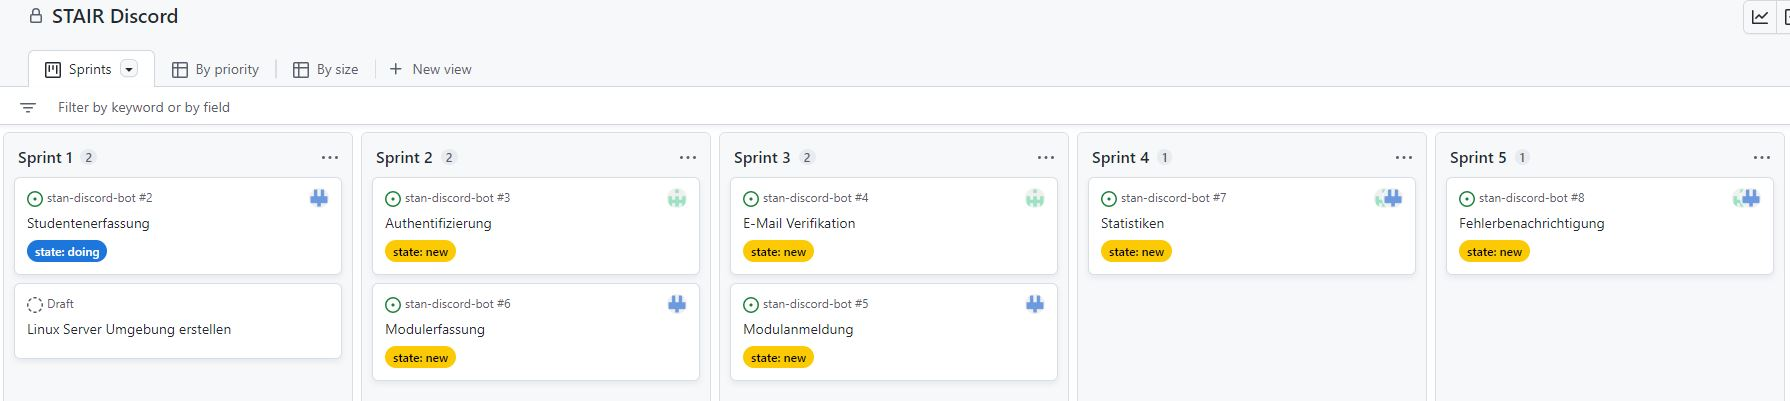
\includegraphics[width=1.3\textwidth]{img/Start_Sprint1_Stories.jpg}
    \caption{Start Sprint 1 User Stories}
    \label{fig:start_sprint_one}
\end{figure}
In der Abbildung erkennt man, dass sich Sprint 1 mit der Studentenerfassung und mit dem Aufsetzen der Linux Umgebung befasst.

\subsubsection{Entity Relationship Diagramm}\label{entity-relationship-diagramm}
Um die Software Architektur richtig planen zu können, muss im Vorfeld festgelegt werden, welche Daten im System wichtig sind und wie diese gespeichert werden. 
Um diesen Zusammenhang richtig darstellen zu können, wird ein Entity-Relationship Diagramm (ERD) erstellt. 
Das ERD kann später in ein Datenbank-Schema übertragen werden. 
Die einzelnen Tabellen sind wie folgt beschrieben.

\begin{figure}[h]
    \centering
    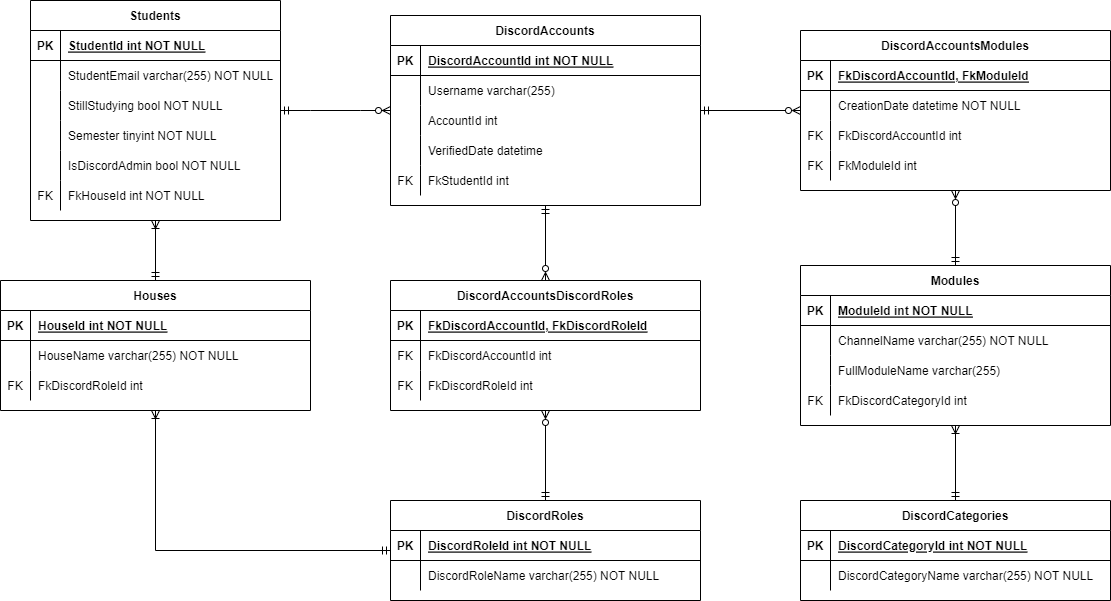
\includegraphics[width=1\textwidth]{img/ER-Diagramm.png}
    \caption{Entity Relationship Diagram}
    \label{fig:ER-Diagram}
\end{figure}

(Ein grosses Bild des Diagramms findet sich im Anhang auf Seite \pageref*{fig:ER-Diagram-big})\\
Bei der Datenspeicherung wird eine Unterteilung zwischen dem Studierenden und seinem Discord Account vorgenommen. 
Dies erlaubt es, eine saubere Trennung zwischen den richtigen Studierenden und ihrem Online-Erscheinen auf Discord zu gewährleisten. 
(Seperation of Concerns (SOC)). 
Die Studierenden Daten, wie Name, Vorname, E-Mail Adresse und Hauszuteilung, werden von der Hochschuladministration zur Verfügung gestellt und können als Liste eingelesen werden. 
Dabei werden die Tabellen \textit{Student} und \textit{House} aufgefüllt und die Zuordnung gemacht. 
Implementiert wird die Funktionalität in diesem Sprint 1 (\nameref{tab: UserStories}).\\
Der \textit{DiscordAccount} wird bei der Authentifikation dem Studierenden zugeordnet.\\
Über die Tabelle \textit{AccountRole}, werden nach dem Authentifizierungsprozess dem Studierenden, die richtigen Rollen zugeordnet.\\
Die Tabelle \textit{Module} wird auch über eine, von der Hochschul-Administration zur Verfügung gestellten Liste befüllt. 
Wenn sich nun der Studierende im Discord beim Bot für ein Modul anmeldet, wird die Zuordnung von Modul und DiscordAccount vorgenommen. 
Der richtige Studierende, \gls{bzw.} seine Daten, haben mit dieser Zuteilung nichts zu tun.\\
Die Tabelle \textit{Category} ist für die technische Umsetzung der Modulgestaltung in Discord nötig. 
Durch die Einschränkung von 50 Channeln in einer Kategorie \ref{discord_einschraenkungen}, können nicht alle Module in einer Kategorie zusammengefasst werden. 
Dies bedeutet, dass die Module aufgeteilt werden müssen. 
In dieser Tabelle werden die Anzahl Kategorien gespeichert.

\subsection{Aufsetzen Solution}
Die C\# Solution wird in drei Projekte aufgeteilt, welche jeweils andere Verantwortlichkeiten haben.
\begin{itemize}
    \item StanBot
    \item StanDatabase
    \item StanScripts
    \item StanDatabaseTest
\end{itemize}

In dem \textbf{StanBot} Projekt wird der Discord Bot erstellt. 
Dort liegt die ganze Funktionalität, welche der Bot braucht, um mit Discord zu kommunizieren. \\
In dem \textbf{StanDatabase} Projekt wird die Datenbank-Anbindung verwaltet. 
Darin werden die Tabellen der Datenbank auf zugewiesene Klassen gemappt. 
Mithilfe der Library LinQ2DB werden die Tabellen der Datenbank dann über diese Klassen verwaltet. 
Datenbank Operationen sollen nur in diesem Projekt erfolgen. 
Die anderen Projekte sollen keinen direkten Zugriff auf die Datenbank haben.\\
Das \textbf{StanScripts} Projekt wird alle Scripte enthalten, die für die Verwaltung des Discord Servers und der Datenbank nötig sind. 
Darin werden sich die Scripte für die Studierende -und Modulerfassung befinden.\\
Im \textbf{StanDatabaseTest} Projekt werden die Tests für die Datenbank geschrieben.
In .NET Applikationen ist es üblich ein eigenes Projekt für die Tests zu erstellen.\autocite{tdykstra_organisieren_nodate}

\newpage
\subsection{Kontextdiagramm}

Diese Darstellung zeigt die wichtigsten Komponenten und wie diese zusammenarbeiten.

\begin{figure}[h]
    \centering
    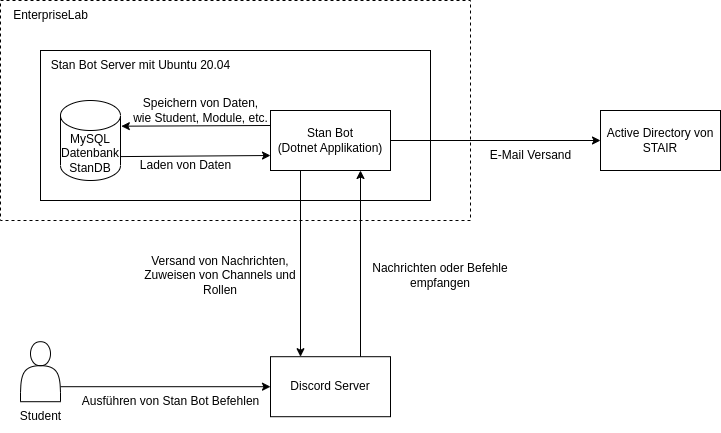
\includegraphics[width=1\textwidth]{img/wipro-stanBotContextDiagram.png}
    \caption{Kontextdiagramm}
    \label{fig:Kontextdiagramm}
\end{figure}

\newpage
\subsubsection{Repository Pattern für die Daten}
Wie im vorherigen Kapitel erwähnt, soll nur das StanDatabase Projekt direkten Zugriff auf die Datenbank haben. 
Wenn der Discord Bot, oder ein Script, Datenbankoperationen ausführen will, wird dazu das Repository Pattern verwendet.
Das Repository Pattern ist dazu da, die Create, Read, Update und Delete (CRUD) Funktionen, welche auf Tabellen durchgeführt werden, zu kapseln. \autocite{gosebrink_aspnet_2014}
Es sieht vor, dass jedes Objekt genau eine Schnittstelle hat, über die Veränderung daran vorgenommen werden können.

\begin{figure}[h]
    \centering
    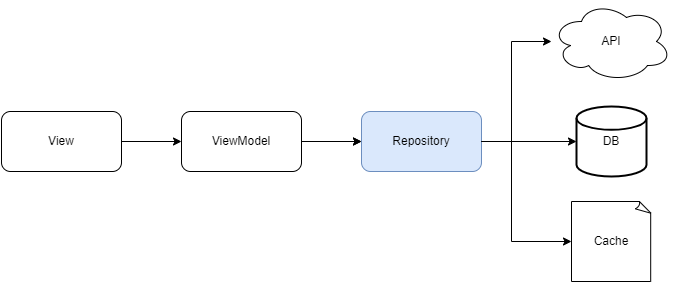
\includegraphics[width=1\textwidth,height=5cm]{img/Repository_Pattern.png}
    \caption{Darstellung Repository Pattern}
    \label{fig:repository_pattern}
\end{figure}

Wie in der Darstellung zu erkennen ist, gibt es für andere Klassen nur noch einen Zugriffspunkt für das gewünschte Datenobjekt.\\
Ein weiterer Vorteil dieses Patterns ist die vereinfachte Testbarkeit. 
Da das Repository selbst eine Schnittstelle, also ein Interface ist, kann es mehrere Implementationen davon geben. 
Für die richtige Applikation kann nun eine Implementation erstellt werden, die wirklich Daten auf der Datenbank verändert, und für das Testen kann eine Implementation erstellt werden, die nur Mock Daten enthält.
Mithilfe von Dependency Injection kann nun jeweils die gewünschte Implementation für das Repository übergeben werden.

\begin{lstlisting}[language=csharp]
// IHouseRepository
public interface IHouseRepository
{
    House GetHouseByName(string houseName);
    bool IsHouseNameValid(string houseName);
}


// HouseRepositoryImpl
public class HouseRepository : IHouseRepository
{
    public House GetHouseByName(string houseName)
    {
        using (var db = new DbStan()) { ... }
    }

    public bool IsHouseNameValid(string houseName)
    {
        using (var db = new DbStan()) { ... }
    }
}

// LoadStudentScript
public class LoadStudents
{
    private readonly IHouseRepository _houseRepository;
    public LoadStudents(IHouseRepository houseRepository)
    {
        _houseRepository = houseRepository;
    }

    public void LoadStudentsFromFile(string filePath)
    {
        ...
        _houseRepository.GetHouseByName(values[houseIndex]);
        ...
    }
}

// Program
public static class Program
{
    public static void Main(string[] args)
    {
        LoadStudents loadStudents = new LoadStudents(new HouseRepository());
        loadStudents.LoadStudentsFromFile(args[1]);
    }
}
\end{lstlisting}

\subsubsection{Studierendenerfassung}
Die Studierenden werden über ein vordefiniertes \gls{CSV} File geladen. 
Nach dem Laden der Datei kann entschieden werden, ob die zuvor erfassten Nutzer als ExStudierende markiert werden und auch sollen. 
Dies ermöglicht es, gleich wie bei den Modulen, Studierende zu ergänzen und zum Start des neuen Semesters die Exstudierenden als solche zu markieren in der Datenbank. 
Zum Schluss muss über Discord noch ein Befehl gestartet werden, um die Rollen auf dem Discord aktualisieren zu können. 
Das \gls{CSV} Format, sowie der Discord- und Konsolen-Befehl werden im Kapitel \nameref{Bedienungsanleitung} genauer beschrieben.

\subsubsection{Aufsetzen der Linux Umgebung}
Der Ubuntu Server wurde vom Enterprise Lab aufgesetzt. 
In der Anleitung im Kapitel \nameref{Bedienungsanleitung} wird die genaue Installation erklärt. 
Bei der Installation stellte MySQL das grösste Problem dar, da dieses ein Standardpasswort setzt, ohne dies dem Nutzer mitzuteilen. 
Dieses muss deshalb mühsam herausgelesen werden aus dem Log Output.

\subsubsection{Verbinden der Datenbank mit Linq2DB}
Die Verbindung zur Datenbank funktioniert über einen Connection String. 
Dieser enthält die Adresse des Datenbank Servers, den dazugehörigen Port, den Datenbank Namen, den Benutzer, das Passwort, sowie das Encoding. 
Das genaue Format wird in der Anleitung im Kapitel \nameref{konfigurationStanBot} beschrieben.

\newpage
\subsection{Sprint 2}
In diesem Sprint wird sich mit der Modulerfassung per Script beschäftigt,
dem Erstellen des Discord Bots und der ersten Kommunikation damit.

\subsubsection{Modulerfassung}
Für die Modulerfassung wird die Liste an Modulen vom Sekretariat benötigt. 
Diese muss dann auf den Server hochgeladen werden und kann dann mithilfe der StanScripts Anwendung eingelesen werden. 
Nach dem Einlesen kann entschieden werden, ob die bereits zuvor erfassten Module gelöscht werden sollen oder nicht. 
Dies ermöglicht es dem Administrator, einzelne fehlende Module nachzuerfassen oder vor dem Start des neuen Semesters die alten, nicht mehr existierenden Module zu entfernen. 
Das Format der einzulesenden \gls{CSV}-Datei wird im Kapitel \nameref{Bedienungsanleitung} geschrieben.

\subsubsection{Aufsetzen Discord Bot}
Um einen Bot zu erstellen, muss man eine Applikation auf der online Discord Developer Plattform kreieren. 
Dort kann man den Namen des Bots angeben und erhält einen Application-Token.

\begin{figure}[h]
    \centering
    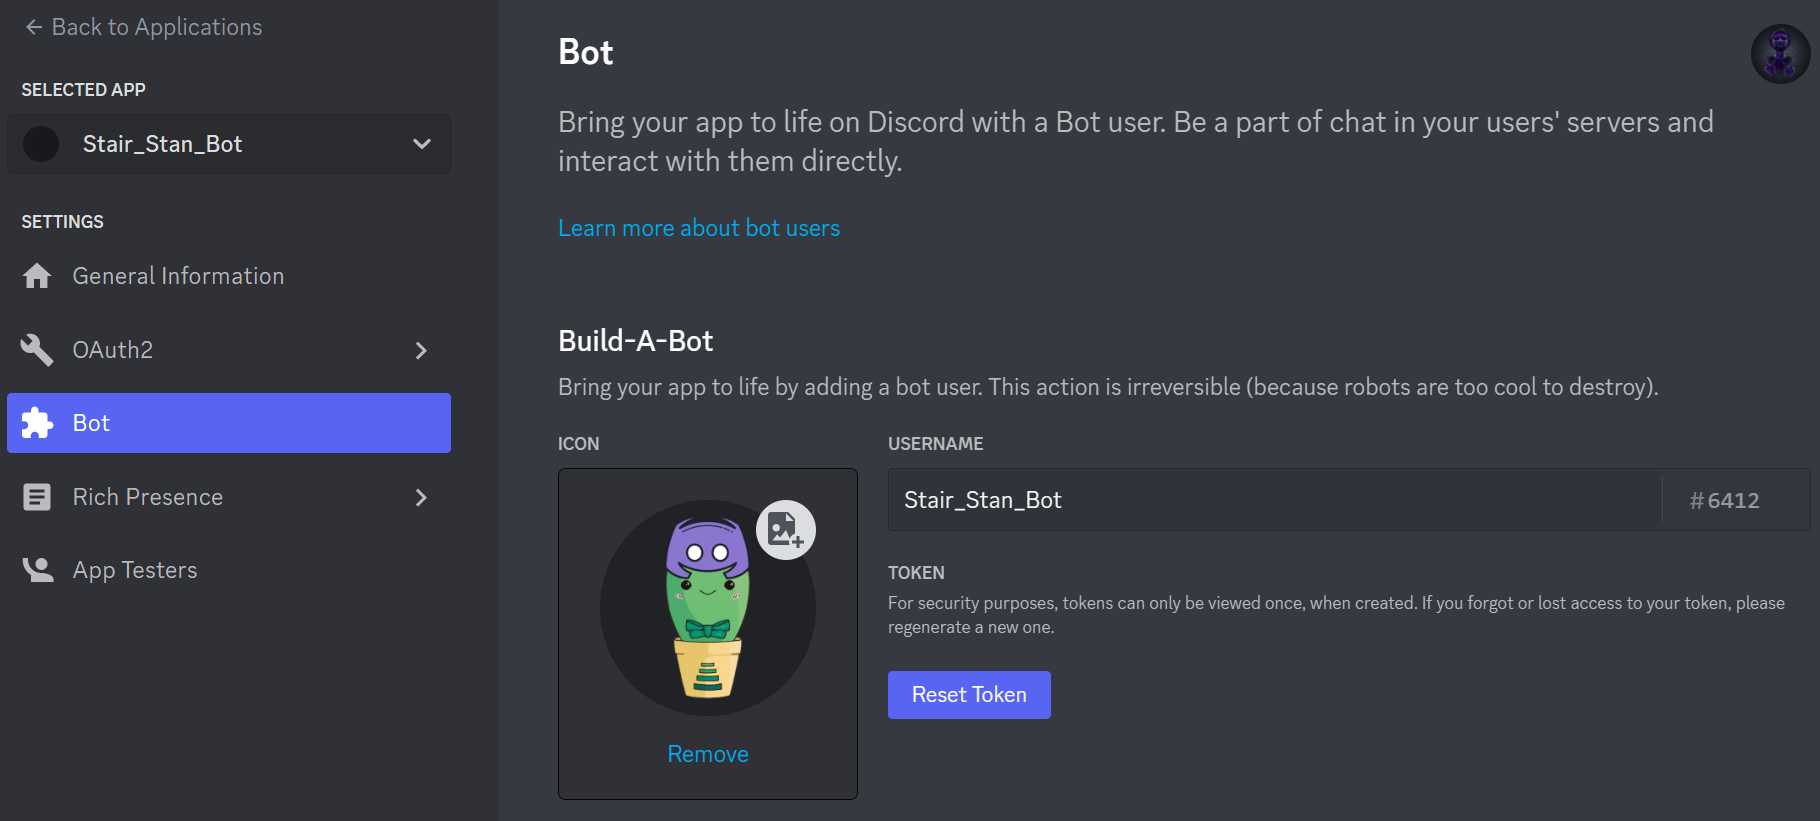
\includegraphics[width=1\textwidth]{img/discord_developer_bot.png}
    \caption{Developer Page Discord Application Token}
    \label{fig:delevoper-application-token}
\end{figure}
Dieses dient als Private Key der Applikation und wird verwendet, um sich im Code mit dem Bot zu verbinden. 
Weiter müssen auf der Plattform die Berechtigungen des Bots spezialisiert werden. 
Dies kann unter dem Tab OAuth2 -> \gls{URL} Generator gemacht werden. 
Die zugewiesenen Berechtigungen müssen gut überlegt sein, da man nur für spezifizierte Events, Callbacks im Code bekommt.
Für dieses Projekt muss die Berechtigung “Administrator” vergeben werden. 
Dies sollte allerdings immer mit Vorsicht genossen werden. 
Da der Stan Bot private Channels erstellen und verwalten soll, benötigt er diese Berechtigung. 
Wenn man die gewünschten Berechtigungen markiert hat, erhält man eine URL. 
Diese kann man direkt im Browser eingeben, um den Bot einem Server zuzuordnen. 
Damit das gelingt, muss der Nutzer auf dem Server die Berechtigung zum Bots hinzufügen besitzen.

\begin{figure}[h]
    \begin{minipage}[t]{0.5\textwidth}
        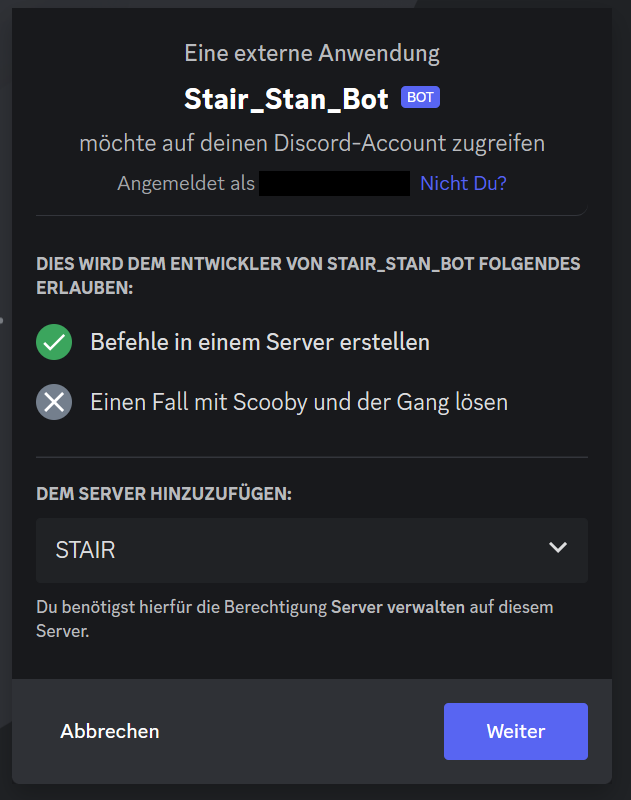
\includegraphics[width=0.7\textwidth]{img/apply_bot_to_server.png}
    \end{minipage}
    \begin{minipage}[t]{0.5\textwidth}
        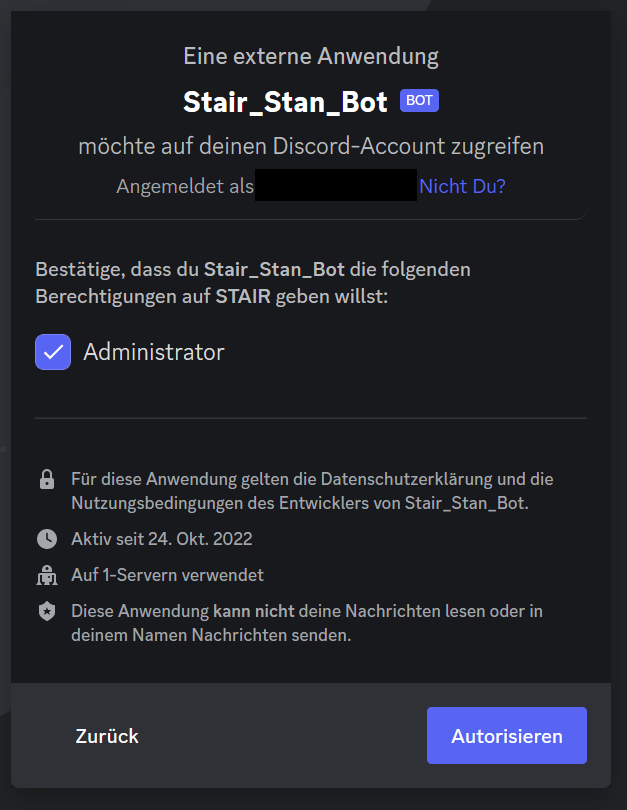
\includegraphics[width=0.7\textwidth]{img/apply_bot_to_server_2.png}
    \end{minipage}
    \caption{Bot dem Server hinzufügen}
    \label{fig:apply-bot-to-server}
\end{figure}

\subsubsection{Stan Bot Architektur}
Grundlegend geht es bei der Bot Architektur um die Kommunikation mit der Discord-Socket-Client Klasse. 
Diese dient als Client-Komponente des Bots und man kann sich dort auf alle Events abonnieren, die Discord anbietet.

\subsubsection*{Services und Dependency Injection}
In der Main-Methode der Applikation wird ein Host Environment für die Applikation erstellt. 
Dieses Environment wird gebraucht, damit der Bot später als Deamon auf der Linux Umgebung im Hintergrund laufen kann. 
Weiter bietet es noch Funktionen zur Dependency Injection an. 
Alle Klassen können dort als Singleton, Scoped oder Transient registriert werden. 
Aus der Microsoft .NET Dokumentation:\autocite{ievangelist_verwenden_nodate}:
\textit{
\begin{itemize}
    \item Transient-Vorgänge sind immer unterschiedliche, und mit jedem Abruf des Diensts wird eine neue Instanz erstellt.
    \item Scoped-Vorgänge ändern sich nur durch einen neuen Bereich, die Instanz ist jedoch innerhalb eines Bereichs immer gleich.
    \item Singleton-Vorgänge sind immer gleich, und eine neue Instanz wird nur einmal erstellt.
\end{itemize}
}

\begin{lstlisting}[language=csharp]
// Program.cs
using IHost host = Host.CreateDefaultBuilder()
            .ConfigureServices((_, services) => services
                .AddSingleton(new DiscordSocketClient())
                .AddSingleton<EventHandler>()
                .AddScoped<IStudentRepository, StudentRepository>()
            .Build();
\end{lstlisting}

In der Bot Klasse kann nun mithilfe eines Providers des Host Environments die Instanz des gebrauchten Services geholt werden.

\begin{lstlisting}[language=csharp]
// Bot.cs
using IServiceScope serviceScope = _hostEnvironment.Services.CreateScope();
IServiceProvider provider = serviceScope.ServiceProvider;
_discordSocketClient = provider.GetRequiredService<DiscordSocketClient>();
\end{lstlisting}

Die Klasse kann aber auch direkt in einen Konstruktor \textit{Injected} werden.
Auf diese Weise hat man an einer Stelle die Kontrolle über alle verfügbaren Klassen und Instanzen.
\begin{lstlisting}[language=csharp]
// EventHandler.cs
public class EventHandler
{
    private readonly DiscordSocketClient _discordSocketClient;
    public EventHandler(DiscordSocketClient discordSocketClient)
    {
        _discordSocketClient = discordSocketClient;
    }
}
\end{lstlisting}

\subsubsection*{Laden der Config}
Beim Starten des Discord Bots muss eine Konfiguration mit spezifischen \textbf{DiscordApplicationToken} mitgegeben werden.
Dieses Application-Token ist wie der private Key der Applikation und sollte nicht veröffentlicht werden. 
Um diese und weitere sensible Informationen einlesen zu können, wird die Config-Klasse erstellt.\\
Diese enthält alle Felder der Settings-Datei und dient als Zugriffspunkt für die sensiblen Informationen. 
Sie liest mit einem einfachen \gls{JSON}-Parser die Settings-Datei ein und setzt ihre Attribute. 
Dabei werden zwei Settingsfiles unterschieden. 
Die erste Settings-Datei enthält Informationen bezüglich des Discord-Servers. 
Die zweite Datei hat Informationen bezüglich der Datenbankverbindung und Einstellungen zum Laden der \gls{CSV}-Daten, wie Studierende und Module.

\subsubsection{Kommunikation mit Discord}
Die Discord.Net Library für C\# implementiert die \textit{DiscordSocketClient} Klasse.
Mit dieser Klasse ist es möglich den Discord Bot zu starten und sich auf Ereignisse zu abonnieren.
Der Bot kann dabei auf dem Server, je nach Berechtigung, fast alle Ereignisse abfangen, die getriggert werden. \\
Das sind nicht nur Ereignisse, die den Bot direkt betreffen, sondern auch allgemeine Sachen, wie schreiben in einem Chat oder dem Beitreten eines Sprach-Channels.
Die Anzahl der Ereignisse, welche abgefangen werden können, hängt von der Einstellung der \textit{GatewayIntents} ab.
Diese und andere Konfigurationen können beim Erstellen des Bots angegeben werden.

\begin{lstlisting}[language=csharp]
// Program.cs
.AddSingleton(new DiscordSocketClient(new DiscordSocketConfig
    {
        GatewayIntents = GatewayIntents.All,
        AlwaysDownloadUsers = true,
        LogLevel = LogSeverity.Debug
    }))
\end{lstlisting}
Allerdings genügt diese Einstellung alleine noch nicht. 
Um Textnachrichten abzufangen, müssen bei der Discord-Developer-Applikation noch die "Privileged Gateway Intents" aktiviert werden. 
Diese werden benötigt, um die Nachrichten der Server Benutzer abzufangen.

\begin{figure}[h]
    \centering
    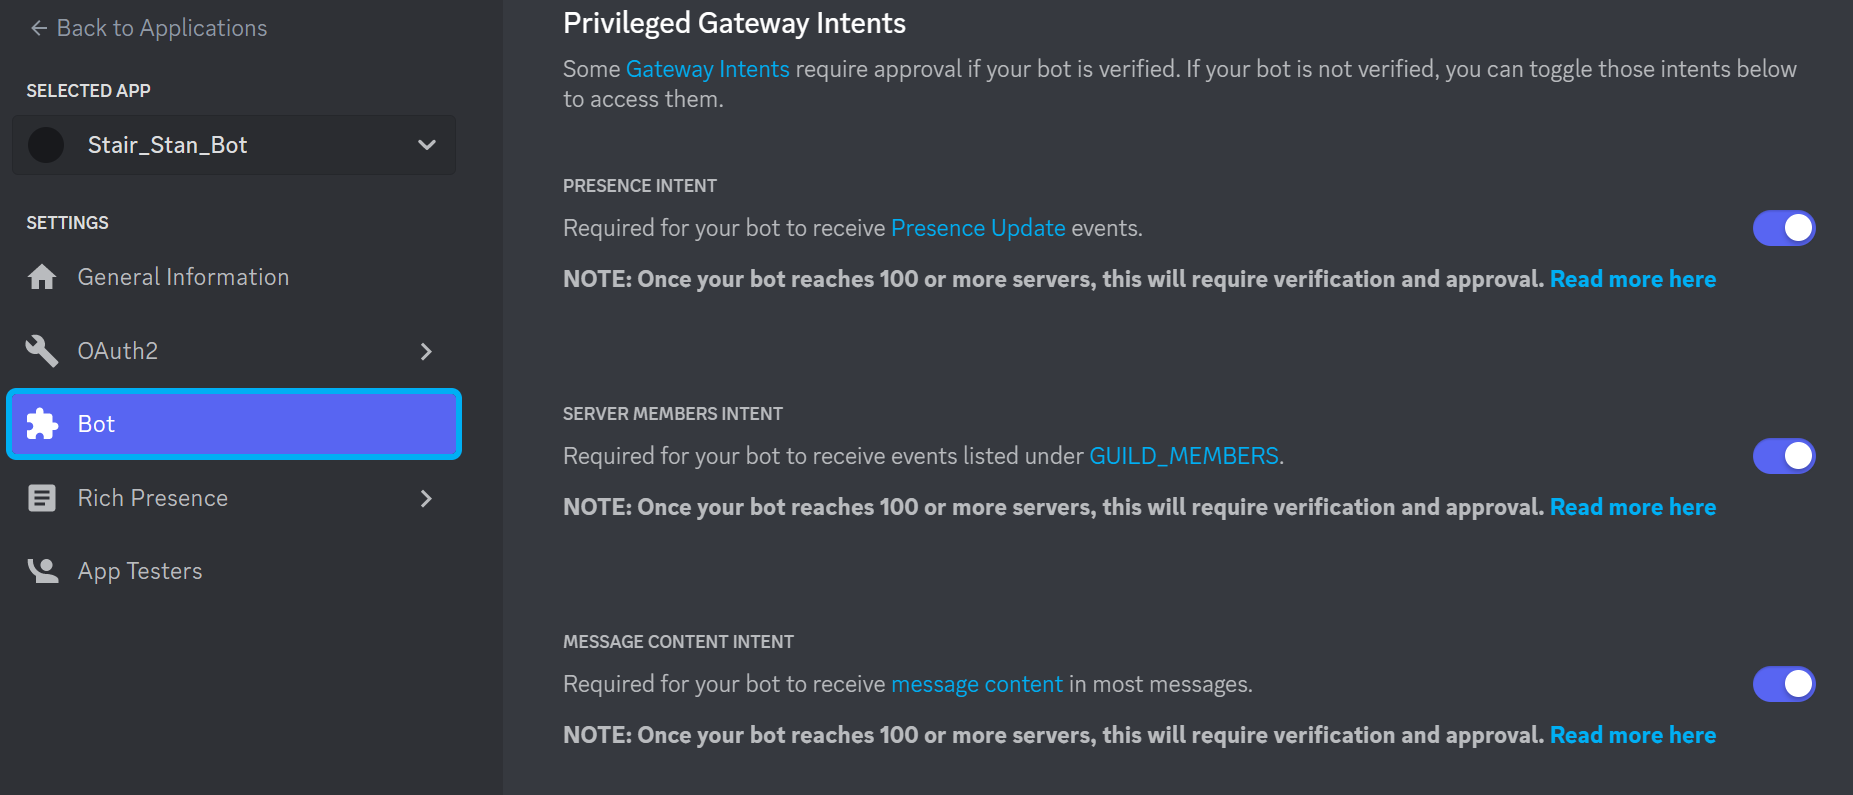
\includegraphics[width=1\textwidth]{img/discord_developer_privileged_intents.png}
    \caption{Privileged Intents für Discord Bot}
    \label{fig:delevoper-privileged-intents}
\end{figure}

Nun können verschiedene Events beim DiscordSocketClient abonniert werden.

\begin{lstlisting}[language=csharp]
// EventHandler.cs
_discordSocketClient.UserJoined += _onUserJoinedEvent.OnUserJoined;
_discordSocketClient.MessageReceived += _messageHandler.OnMessageReceived;
\end{lstlisting}

Es wird für jedes Event eine eigene Klasse erstellt. 
So können diese schön gekapselt und separat behandelt werden.\\
Wie man im Code sehen kann, gibt es für den Discord-Socket-Client nur ein MessageReceived Event. 
Dieses Event entscheidet noch nicht, ob es sich um eine allgemeine Nachricht im Chat handelt, eine direkte Nachricht an den Bot oder einen Befehl.
Im Anhang auf Seite \pageref*{fig:message-handling} findet man das Klassendiagramm zum Thema Message Handling.\\\\
Um jetzt nicht alle Nachrichten in einer Klasse bearbeiten zu müssen, wird auf die Hilfe von Interfaces zurückgegriffen.
Alle Nachrichten werden an die \textit{MessageHandler} Klasse weitergeleitet. 
Dort wird eine Vorselektion gemacht, ob es sich bei den eintreffenden Nachrichten um System Messages handelt oder um andere Bot Nachrichten. 
Wird diese Vorselektion nicht gemacht, kann es sein, dass es zu einer Endlosschleife führt, da der Bot auch seine eigenen geschriebenen Nachrichten in der \textit{MessageReceived} Methode empfängt.\\
Im Anschluss wird jede Implementation der \textit{IMessageReceiver} Klasse durchgegangen und überprüft, ob die MessageSource korrekt ist und die \textit{IsMatch} Methode true zurückgibt. 
Nur wenn beide Anforderungen erfüllt sind, wird die Nachricht an die jeweilige Message Receiver Implementation weitergeleitet.

\subsubsection*{Das EmailMessageReceivedEvent}
Die \textit{EmailMessageReceivedEvent}-Klasse implementiert das \textit{IMessageReceived}-Interface und ist somit ein Empfänger des MessageReceived Events von Discord. 
In der \textit{EmailMessageReceivedEvent} Klasse wird eine Nachricht als Direct Message erwartet. 
Sie soll die Form \textit{<vorname.name>@stud.hslu.ch} oder \textit{<vorname.name>@hslu.ch} haben. 
Alle Nachrichten, die nicht diesem Muster entsprechen, werden nicht behandelt. 
Dies erlaubt es nur Mitarbeitern oder Studierenden der Hochschule, sich im Discord Server zu authentifizieren.\\\\
Sobald die Nachricht diesem Muster entspricht, wird sie der \textit{ProcessMessage} Methode übergeben.
Dort wird zuerst in der Datenbank überprüft, ob der Nutzer vorhanden ist. 
Falls nicht, wird eine Fehlermeldung an den Nutzer zurückgegeben. 
Wenn alles stimmt, wird ein Code für die Verifikation generiert.\\
Bei der Generierung des Codes wird eine zufällige 6 stellige Zahl erstellt und diese, zusammen mit der Discord Author ID, in einer Liste gespeichert. 
Solange der Server online ist, werden offene Authentifikation in dieser Liste persistiert. 
Falls der Server aus einem unerklärlichen Grund heruntergefahren wird oder die Applikation neu gestartet wird, muss der Authentifizierungsprozess von neuem begonnen werden. 
Dies wird allerdings in Kauf genommen, da noch nichts von Bedeutung für den Benutzer oder den Server passiert ist.\\\\
Sobald der Code generiert wird, wird dieser, zusammen mit einer Nachricht, dem Benutzer an die angegebene E-Mail Adresse gesendet und eine Nachricht an den Benutzer zurückgegeben. \\
Damit ist dieser Schritt abgeschlossen.

\subsubsection*{Das VerificationCodeMessageReceivedEvent}
Die \textit{VerificationCodeMessageReceivedEvent}-Klasse implementiert auch das \textit{IMessageReceived}-Interface. 
Damit eine Nachricht an diese Klasse weitergeleitet wird, muss es auch eine Direct Message an den Bot sein, sowie eine 6-stellige Zahl. 
Diese Überprüfung wird mit dem Regex-String "\textbf{\^[0-9]\{6\}\$}" erreicht. 
Wenn die Nachricht dem korrekten Muster entspricht, wird in der Liste im VerificationCodeManager überprüft, ob eine offene Authentifizierung von diesem Nutzer mit diesem Code existiert. 
Falls dies nicht der Fall ist, wird eine Fehlermeldung an den Nutzer zurückgegeben.\\\\
Wenn der Code korrekt ist, wird in der Datenbank ein neuer \textbf{DiscordAccount} erstellt. 
Dieser wird mit dem zugehörigen Studierenden mithilfe der E-Mail verbunden. 
Des Weiteren wird in der Zwischentabelle \textbf{DiscordAccountDiscordRole} die Verbindung zu den Rollen erstellt. 
Für neu authentifizierte Studierende wird die Rolle \textbf{student} und die richtige Haus-Rolle zugewiesen.\\\\
Sobald die Manipulationen auf der Datenbank abgeschlossen sind, werden die Änderungen auch auf den Discord übertragen. 
Der Studentierende bekommt dort vom Bot die Rollen zugewiesen. Damit hat er jetzt vollen Zugang zum STAIR-Server.\\\\
Im Falle, dass der Nutzer sich schon einmal auf dem STAIR Server authentifiziert hat, aber aus irgendeinem Grund den Server verlassen hat, muss er sich noch einmal authentifizieren. 
Allerdings werden keine Datenbankmanipulationen gemacht, sondern die Rollen, welcher er ja schon besitzt, zurückgegeben.

\newpage
\subsection{Sprint 3}
In diesem Kapitel setzen wir uns mit der Command Service Architektur von Discord auseinander. 
Im Weiteren wird die Implementation der show- und hide Module- Commands genauer erklärt.

\subsubsection{Command Service Architektur}
Der Command Service wird von Discord verwendet, um Befehle an den Bot zu schicken. 
Der Service wird unabhängig neben dem Discord Client gestartet, aber nimmt diesen beim Ausführen der Commands als Kontext entgegen.

\subsubsection*{Starten des Command Service}
Der Command Service wird wie folgt dem Hosting Environment hinzugefügt.

\begin{lstlisting}[language=csharp]
// Program.cs

.AddSingleton(new CommandService(new CommandServiceConfig
    {
        DefaultRunMode = RunMode.Async,
        LogLevel = LogSeverity.Debug
    }))
\end{lstlisting}
Beim Starten des Event Handlers wird der Command Service initialisiert. 
Durch die Methode \textbf{AddModulesAsync} geht der Command Service automatisch durch die ganze Projektstruktur durch und sucht nach Klassen, welche von \textit{ModuleBase<SocketCommandContext>} erben. 
Diese fügt er dem Context, in dem der Bot läuft, hinzu.

\begin{lstlisting}[language=csharp]
// EventHandler.cs

await _commandService.AddModulesAsync(Assembly.GetEntryAssembly(), provider);
\end{lstlisting}

\subsubsection*{Der CommandMessageReceivedEvent}
Die Befehle, welche der Nutzer schicken kann, werden als normale Nachrichten verarbeitet. 
Dies bedeutet, dass sie auch durch die \textbf{MessageReceived} Methode abgefangen werden. 
In der \textit{CommandMessageReceivedEvent}-Klasse werden alle Nachrichten mit dem Command-Präfix verarbeitet. 
Dieser ist in der Config Datei hinterlegt und kann geändert werden. 
Für das Projekt wird der Präfix \textbf{!} verwendet. 
Falls eine Nachricht mit diesem Präfix eintrifft, wird mit folgender Anweisung versucht, diesen Befehl auszuführen.

\begin{lstlisting}[language=csharp]
// CommandMessageReceivedEvent.cs

var context = new SocketCommandContext(_discordSocketClient, message);
var result = await _commandService.ExecuteAsync(context, argPos, _serviceProvider);
\end{lstlisting}
Nun schaut der Command Service durch alle Commands durch, welche er im vorherigen Schritt mit der \textbf{AddModulesAsync} Methode hinzugefügt hat. 
Falls er diesen Command nicht erfolgreich ausführen kann, gibt er eine Fehlermeldung zurück, die wiederum in geeigneter Form den Benutzer mitgeteilt wird.

\subsubsection*{Command-Klassen erklärt}
Die Command Klassen erben, wie im vorherigen Kapitel erklärt, von\\ \textbf{ModuleBase<SocketCommandContext>}. 
Dadurch werden alle Methoden, welche in der Klasse mit einem \textbf{[Command()]} Attribut versehen sind, dem Command Service hinzugefügt.

\begin{lstlisting}[language=csharp]
// Miscellaneous.cs

public class Miscellaneous : ModuleBase<SocketCommandContext>
{
    [Command("ping")]
    [Alias("latency")]
    [Summary("Displays the bot's current latency")]
    public Task PingCommand() => ReplyAsync($"Pong! The bot's latency is {Context.Client.Latency} ms.");
}
\end{lstlisting}
Der Text, welcher im Command-Attribut steht, ist der Befehl, den der Benutzer im Discord ausführen muss. 
Im obigen Beispiel wäre dies: \textbf{!ping}.\\
Je nach Anwendungsfall können noch weitere Attribute ergänzt werden. 
So wird oben ein Alias und eine Beschreibung hinzugefügt. 
Es können aber auch Berechtigungsfragen schon mit diesen Rollen abgeklärt werden. 
Beispielsweise gibt es ein \textbf{[RequireRole()]} - Attribut, welches eine bestimmte Rolle zum Ausführen des Commands vorgibt. 
Befehle können auch Argumente entgegennehmen. 
Diese werden einfach als Argumente im Methodenkopf angegeben. 
Falls mehrere Parameter verwendet werden müssen, muss das Attribut \textbf{[Remainder]} hinzugefügt werden. 
Dies verhindert, dass nur das letzte Argument an den Bot übertragen wird.\\\\
Der \textbf{Context} wird von ModuleBase geerbt. 
Dadurch können der Channel oder der Benutzer, der den Befehl geschickt hat, abgefragt werden. 
Dies erweist sich als nützlich, wenn gewisse Befehle nur in gewissen Channeln abgesetzt werden dürfen.\\\\
Für den Anfang wurde ein \textbf{!ping} Befehl und ein \textbf{!help <command>} Befehl hinzugefügt. 
Der \textbf{!ping}-Befehl gibt die aktuelle Antwortzeit des Bots zurück. 
Beim !help-Befehl werden alle Commands, welche registriert sind, aufgelistet. 
Es kann auch ein \textbf{!help <command>} Befehl ausgeführt werden, um detaillierte Informationen zu einem Befehl zu erhalten.

\newpage
\subsubsection{show/hide <module> Command}
Die beiden Commands show und hide können von Studierenden benutzt werden, um sich selbst zu einem Modul Discord Channel hinzuzufügen um sich dann über das Modul austauschen zu können. 
Der Name des Moduls muss hierfür spezifisch formatiert sein. 
Eine Anleitung hierzu wird den Studierenden auf dem Channel zum Anmelden bei den Modulen angezeigt. 
Diese Anleitung wird gepinnt, damit sie zwischen den vielen Nachrichten nicht untergeht.\\
Der angegebene Modulname muss dem Kurznamen entsprechen. 
Gross- und Kleinschreibung darf ignoriert werden, da im Hintergrund dies einheitlich umgewandelt wird. 
Einige Module haben am Ende des Kurznamens eine Erweiterung, um die verschiedenen Durchführungen, \gls{z.B.} bei verschiedenen Professoren, zu unterscheiden. 
Auch der Präfix und Suffix müssen entfernt werden, welche den Studiengang \gls{bzw.} das Jahr und das Semester beinhalten.\\
Beispiele:

\begin{table}[h]
    \centering
    \begin{tabular}{|l|l|l|}
        \hline
        \rowcolor[gray]{.9} Angezeigt bei Modulbeschrieb & Angezeigt im MyCampus (Stundenplan) & Beispiel Befehl \\
        \hline
        GAMEDEV & I.BA\_GAMEDEV.H2201 & show gamedev \\
        \hline
        3DMOD4RT & I.BA\_3DMOD4RT.21 & show 3dmod4rt \\
        \hline
        LIAL & I.BA\_LIAL\_E.F2201 & show lial \\
        \hline
    \end{tabular}
    \caption{Show und Hide Command Beispiele}
    \label{tab: Show und Hide Command Beispiele}
\end{table}
Diese Umwandlung muss ebenfalls beim Laden der Modul-Liste des Sekretariats durchgeführt werden. 
Diese automatische Umwandlung wird durch Unit Tests getestet. 
Genauere Angaben zu den Tests werden im Kapitel \nameref{Teststrategie} beschrieben. 
Die Abkürzungen können Studierende über die Modulliste der HSLU herausfinden und wird gleich hinter dem vollen Namen angezeigt.\autocite{noauthor_bachelor_nodate} \\

\begin{figure}[hb]
    \centering
    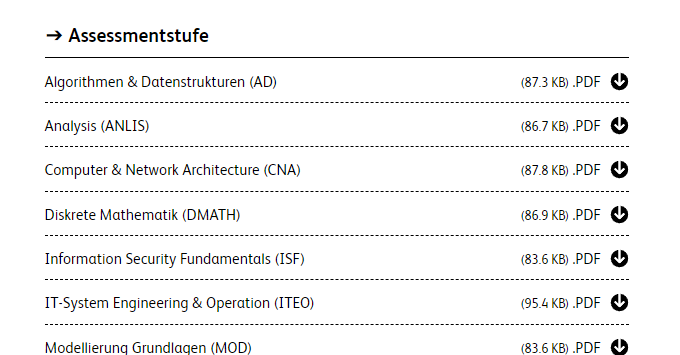
\includegraphics[width=0.8\textwidth]{img/ausschnittModullisteHsluInformatik.PNG}
    \caption{Ausschnitt der Modulliste des Informatik Studiengangs}
    \label{fig:modulliste-informatik}
\end{figure}
\clearpage

\subsubsection{E-Mail Service}
Der E-Mail Service wird im Authentifizierungsprozess benötigt. 
Der Nutzer bekommt eine E-Mail mit dem Verifizierungscode an die angegebene Studierendenadresse gesendet. 
Diesen Code muss er an den Bot zurücksenden, um die Authentifizierung abzuschliessen.\\\\
Es wird über verschiedene Lösungen zu diesem Problem diskutiert.
So kann man beispielsweise einen eigenen Mail-Server hosten und die Mails über diesen versenden.  
Oder man nutzt die bestehende Lösung des alten Stan Bots.\\
Für dieses Projekt wird entschieden, die bestehende Lösung weiter zu nutzen. 
Dies aus dem Grund, dass der Mail Service etabliert ist, funktioniert und die Infrastruktur schon besteht. 
Für das Team besteht kein Grund, diesen zu ersetzen.\\\\
Um Mails aus einer Applikation verschicken zu können, müssen diese über einen Account auf einem Mail Server verschickt werden. 
Man muss sich also mit einen Mail Server verbinden, um dort mit einem registrierten E-Mail Account die Mail versenden zu können. 
Um dieses Problem zu lösen, wird mit den Angeboten von Microsoft gearbeitet.\\
Als Mail Server wird Outlook verwendet, da alle Studierenden ein Microsoft Konto besitzen und ihre E-Mails über Outlook verwalten. 
Auch STAIR nutzt Outlook, um ihre E-Mails zu versenden.

\subsubsection*{Mircosoft Identity \& Microsoft Azure}
Die Microsoft Identity Plattform erlaubt es Entwicklern, einen Authentifizierungsmechanismus in ihre Applikation einzubauen. 
Für Besitzer eines Microsoft Azure Administrator Kontos oder Office 365 ist die Lösung kostenlos und da auch STAIR einen Office 365 Account hat, bietet sich diese Lösung an. 
Die Microsoft Identity Plattform baut auf der OpenId Technologie auf und kann damit jeden OpenId Connect Provider hinzufügen, \gls{bzw.}  diesen nutzen. 
Um einer Applikation diese Authentifizierungsmechanismen hinzuzufügen, muss in Microsoft Azure eine Applikation erstellt werden. 
Anschliessend können Berechtigungen für die Nutzer und die Applikation eingestellt sowie die App-ID herausgelesen werden. \autocite{noauthor_introduction_nodate}
Dies sieht man auf folgender Abbildung.

\begin{figure}[h]
    \centering
    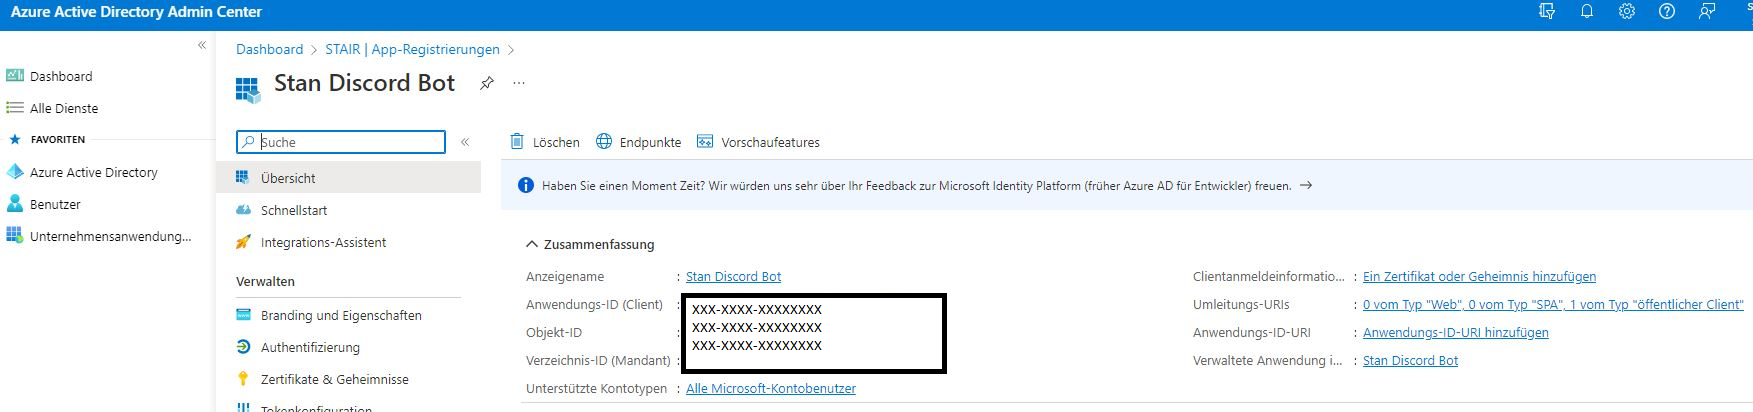
\includegraphics[width=1\textwidth]{img/azure_discord_app_blacked.png}
    \caption{Azure Discord App Registration}
    \label{fig:azure-discord-app-registration}
\end{figure}
Wenn man die Authentifizierungsmöglichkeiten bei der registrierten App aktiviert, wird automatisch Microsoft Identity verwendet.\\\\
Für den Discord Bot wurde von Microsoft Identity die Microsoft Authentication Library (MSAL) benutzt.\autocite{dickson-mwendia_initialize_nodate}
Diese ist Teil von Microsoft Identity. 
Damit kann man sich einen Client erstellen, mit dem man sich authentifizieren kann.

\begin{lstlisting}[language=csharp]
// DeviceCodeAuthProvider.cs
_msalClient = PublicClientApplicationBuilder
                .Create(appId)
                .WithAuthority(AadAuthorityAudience.AzureAdAndPersonalMicrosoftAccount, true)
                .Build();
\end{lstlisting}

Dem \textit{PublicClientApplicationBuilder} kann man die Anwendungs-ID mitgeben, welche man auf der registrierten Azure Applikation auslesen kann. 
Im Anschluss wird ausgewählt, wie man sich identifizieren möchte. 
Microsoft Identity bietet die gängigen Authentifizierungsmöglichkeiten an. 
So kann man sich mit dem Microsoft Konto anmelden oder aber über Third-Party Anbindungen authentifizieren. 
Dies nennt Microsoft, Hybrid Identity.\autocite{billmath_what_nodate}
Für den Discord Bot wird das Gerät, auf dem die Applikation läuft, beim Starten einmalig authentifiziert und man erhält einen Access Token zurück. 
Dieses wird im nächsten Schritt für die Kommunikation mit der Microsoft Graph API verwendet.

\subsubsection*{Microsoft Graph}
Microsoft Graph ist eine \gls{REST} Schnittstelle von Microsoft, mit dazugehörigen Clientbibliotheken. 
Mit diesen kann man alle Microsoft-Services ansprechen. \autocite{angelgolfer-ms_microsoft_nodate}
Diese REST Schnittstelle kann man aus der eigenen Applikation aufrufen, um zum Beispiel über die Azure Applikation eine E-Mail zu versenden. 
Microsoft Graph läuft in der Grundlage mit einem authentifizierten Benutzer oder Gruppen. 
So kann man über die REST Schnittstelle, sich zu jeder seiner Microsoft Anwendungen, Daten beschaffen.\\\\
Das Token, welches man von nach der Authentifikation mit Microsoft Identity erhält, kann nun der Klasse \textbf{GraphServiceClient} übergeben werden. 
Der GraphServiceClient ist Teil von Microsoft Graph und erlaubt es über die Graph API, REST Endpunkte aufzurufen. 
So kann eine Post Request auf den Endpunkt \textit{https://graph.microsoft.com/v1.0/me/sendMail} gesendet werden. 
In der Applikation wird der Request wie folgt aussehen.

\begin{lstlisting}[language=csharp]
// MailServicce.cs
await _graphServiceClient.Me.SendMail(message).Request().PostAsync();
\end{lstlisting}

Da der GraphServiceClient mit dem richtigen Microsoft Konto authentifiziert ist, werden nun die E-Mails direkt über das richtige Outlook Konto weitergeleitet.

\begin{figure}[h]
    \centering
    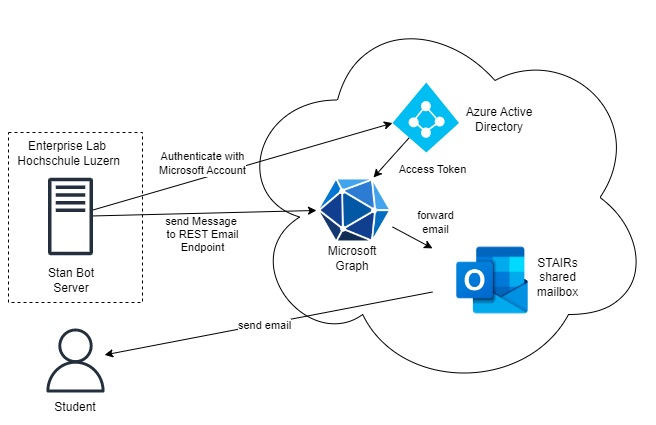
\includegraphics[width=1\textwidth]{img/Email_Infrastruktur.png}
    \caption{Email Versand Infrastruktur}
    \label{fig:send-email-infrastructure}
\end{figure}

\newpage
\subsection{Sprint 4}
In diesem Sprint werden die Statistiken für die STAIR Administration und ihre Mitglieder implementiert.

\subsubsection{Statistiken}
In den Anforderungen wird gewünscht, dass man als STAIR Mitglied mithilfe der Datenbank verschiedene Statistiken auslesen kann. 
Die Art, wie man diese Statistiken erhält, kann selbst entschieden werden. 
Das Team hat entschieden, diese über Bot Commands zu erstellen. 
Mit den Commands ist es möglich, Befehle für den Bot zu übergeben. 
Da dieser über das Repository Pattern Zugriff auf die Datenbank hat, kann er die gewünschten Queries absetzen.\\
Eine weitere Möglichkeit wäre gewesen, Statistiken mithilfe von Scripts abzufragen. 
Mit dieser Methode muss man sich allerdings auf den Server im Enterprise Lab verbinden, die Scripts heraussuchen und diese dort ausführen. 
Dies wird als nicht leicht erweiterbar und benutzerfreundlich eingestuft und aus diesem Grund verworfen.\\\\
Für dieses Projekt werden 4 verschiedene Statistiken implementiert. 
Weitere können aber einfach hinzugefügt werden. \\
Die 4 Statistiken sind:
\begin{itemize}
    \item Anzahl Studenten Pro Haus
    \item Anzahl Studenten pro Semester
    \item Anzahl registrierter Discord Accounts mit Studenten aus jeweiligem Semester
    \item Anzahl Mitglieder pro Modul-Channel
\end{itemize}
Die Befehle werden in Discord wie folgt abgesetzt:
\begin{itemize}
    \item \textbf{!studentsPerHouse}
    \item \textbf{!studentsPerSemester}
    \item \textbf{!accountsPerSemester}
    \item \textbf{!membersPerModule}
\end{itemize}
Die Abfragen werden in den weiteren Kapiteln noch genauer beschrieben.

\subsubsection*{Aufruf Berechtigungen}
Es sollen nur Administratoren und STAIR Mitglieder diese Commands einsehen und ausführen können. 
Dazu wird bei den Commands das Attribute [RequireRole("stair")] und [RequireRole("administrator")] gebraucht. 
Diese Attribute haben allerdings nicht funktioniert. 
Es konnten immer noch Mitglieder ohne diese Rollen die Commands absetzen.\\
Deshalb wird eine andere Lösung implementiert. 
Auf Discord wird dabei ein \textbf{\#bot-commands} Text-Channel erstellt. 
Auf diesen haben nur die Administratoren und STAIR-Mitglieder Zugriff. 
Der Bot führt die Befehle jetzt nur aus, wenn sie von diesem Channel versendet werden.

\subsubsection*{Plotting Library}
Damit Statistiken einfacher verständlich und aussagekräftig sind, weden Diagramme verwendet. (engl. Plots). 
Plotting Libraries gibt es viele, doch es wurde sich für das kostenlose OpenSource Projekt ScottPlott entschieden. 
ScottPlot ist für .NET entwickelt und liefert viele verschiedene Chart-Möglichkeiten, die einfach erstellt und bearbeitet werden können. 
Die Verwendung ähnelt sehr der Library Matplotlib und ist dadurch für Personen, die sich schon mit Statistiken im Programmieren beschäftigt haben, einfach zu lernen. 
Sie bieten alle bekannten Diagramm-Arten an und erlauben es auch, interaktive Plots zu erstellen.\autocite{noauthor_scottplot_nodate}

\newpage
\subsubsection*{Statistik: Students per house}
In dieser Statistik werden die Anzahl Studenten pro Haus zurückgegeben.
Grundlage dafür bietet folgende SQL Query:

\begin{lstlisting}[language=SQL]
SELECT HouseName, Count(s.StudentId) AS StudentCount
FROM students AS s
INNER JOIN houses AS h ON s.FkHouseId=h.HouseId
GROUP BY h.HouseName;
\end{lstlisting}

Übersetzt in eine Linq Query ergibt sich folgendes.

\begin{lstlisting}[language=SQL]
// StudentRepository.cs

from s in db.Student
join h in db.House on s.FkHouseId equals h.HouseId
group s by h.Name into g
select new StudentsPerHouseDTO
{
    HouseName = g.Key,
    StudentsCount = g.Count()
};
\end{lstlisting}

Dargestellt wird diese Abfrage in einem Bar-Plot, wobei die x-Achse die verschiedenen Häuser sind und die y-Achse die Anzahl Studierende in einem Haus. 
Die einzelnen Bars werden nach den Farben des Hauses dynamisch eingefärbt.

\begin{figure}[h]
    \centering
    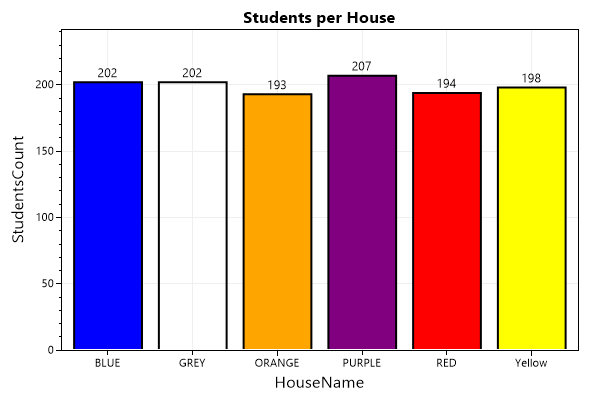
\includegraphics[width=0.8\textwidth]{img/studentsPerHouse.png}
    \caption{Students per house}
    \label{fig:students-per-house}
\end{figure}

\newpage
\subsubsection*{Statistik: Students per semester}
In dieser Statistik wird die Anzahl Studierende in den verschiedenen Semestern zurückgegeben. 
Die Anzahl der Semester wird bestimmt durch die registrierten Studierenden in der Liste der Hochschuladministration.\\
Die grundlegende SQL Query ist folgende:

\begin{lstlisting}[language=SQL]
SELECT Semester, Count(s.StudentId) AS StudentCount
FROM students AS s
GROUP BY s.Semester;
\end{lstlisting}

Übersetzt als Linq Query ergibt sich folgendes.

\begin{lstlisting}[language=SQL]
// StudentRepository.cs

from s in db.Student
group s by s.Semester into g
select new StudentsPerSemesterDTO
{
    Semester = g.Key,
    StudentsCount = g.Count()
};
\end{lstlisting}

Die Abfrage wird als Bar-Plot dargestellt. 
Auf der x-Achse befinden sich die verschiedenen Semester und auf der y-Achse die Anzahl der sich darin befindenden Studierende.

\begin{figure}[h]
    \centering
    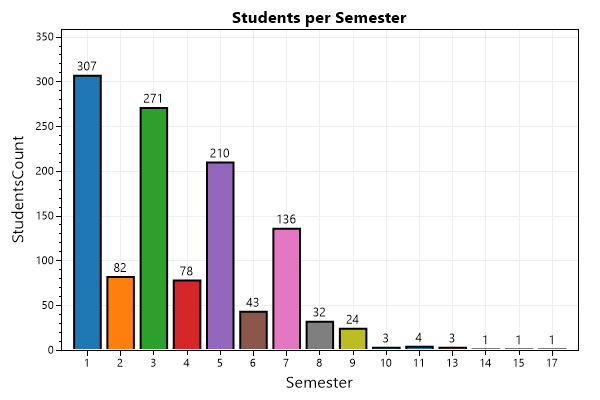
\includegraphics[width=0.8\textwidth]{img/studentsPerSemester.png}
    \caption{Students per semester}
    \label{fig:students-per-semester}
\end{figure}

\newpage
\subsubsection*{Statistik: Accounts per semester}
In dieser Statistik kann die Anzahl der sich im STAIR Discord Server authentifizierten Personen abgefragt werden. 
Gruppiert wird dabei wieder nach dem Semester, in dem sich der Studierende befindet. 
So kann herausgefunden werden, in welchen Semestern sich die Discord Benutzer durchschnittlich befinden. 
Die grundlegende SQL Query ist folgende:

\begin{lstlisting}[language=SQL]
SELECT s.Semester, Count(ac.FkStudentId)
FROM discordaccounts AS ac
RIGHT JOIN students AS s ON ac.FkStudentId=s.StudentId
GROUP BY s.Semester;
\end{lstlisting}

Diese Query ist etwas schwieriger in Linq zu übersetzen, da es so etwas wie \textbf{RIGHT JOIN}  in Linq nicht gibt. 
Stattdessen müssen die Aufrufe der Tabellen in der Query vertauscht werden. 
Also die Tabelle, welche man mit \textbf{RIGHT JOIN}  ganz anzeigen möchte, muss zuerst selektiert werden. 
Im Anschluss wird dann die andere gejoint.
Damit auch leere Felder angezeigt werden, also z.B. Semester, in denen es keine registrierten Studierenden gibt, muss der Befehl \textit{DefaultIfEmpty()} auf der gejointen Gruppe aufgerufen werden.

\begin{lstlisting}[language=SQL]
// DiscordAccountRepository.cs

from s in db.Student
join dc in db.DiscordAccount on s.StudentId equals dc.FkStudentId into joinGroup
from gr in joinGroup.DefaultIfEmpty()
group gr by s.Semester into g
select new DiscordAccountsPerSemesterDTO
{
    Semester = g.Key,
    AccountsCount = g.Count(stud => stud.FkStudentId != null)
};
\end{lstlisting}

Diese Abfrage wird, wie die vorherige, auch als Bar-Plot dargestellt. 
Auf der x-Achse befinden sich die verschiedenen Semester und auf der y-Achse die Anzahl der authentifizierten Studierenden.

\begin{figure}[h]
    \centering
    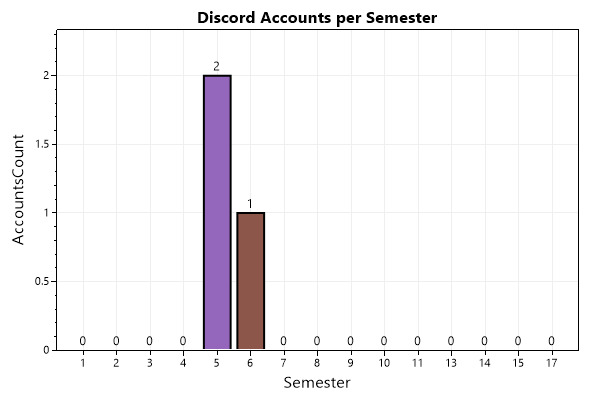
\includegraphics[width=0.6\textwidth]{img/accountsPerSemester.png}
    \caption{Accounts per semester}
    \label{fig:accounts-per-semester}
\end{figure}

\clearpage
\subsubsection*{Statistik: Members per module}
In dieser Statistik können die meistabonnierten Modul Channels abgefragt werden. 
Es wird also nach den meisten Mitgliedern sortiert. 
Die Anzahl der Module, die im Chart angezeigt werden sollen, ist über einen Parameter nach dem Befehl einstellbar. 
Standardmässig ist die Anzahl Module auf 10 eingestellt.\\
Die grundlegende SQL Query ist folgende:

\begin{lstlisting}[language=SQL]
SELECT m.ChannelName, Count(am.FkDiscordAccountId) AS MemberCount
FROM discordaccountsmodules AS am 
INNER JOIN modules AS m ON am.FkModuleId=m.ModuleId
GROUP BY m.ChannelName
ORDER BY MemberCount DESC;
\end{lstlisting}

Übersetzt als Linq Query ergibt sich folgendes.

\begin{lstlisting}[language=SQL]
// DiscordAccountModuleRepository.cs

from am in db.DiscordAccountModule
join m in db.Module on am.FkModuleId equals m.ModuleId
group m by m.ChannelName into g
orderby g.Count() descending
select new MembersPerModuleDTO
{
    ModuleName = g.Key,
    MemberCount = g.Count()
};
\end{lstlisting}

Diese Abfrage wird als Kuchen-Diagramm dargestellt. 
So können die Proportionen der einzelnen Module besser erahnt werden. 
Die Anzahl der Mitglieder dieser Channels wird in den Kuchenstücken angezeigt. 
Die Legende rechts bietet eine Übersicht der dargestellten Module.

\begin{figure}[h]
    \centering
    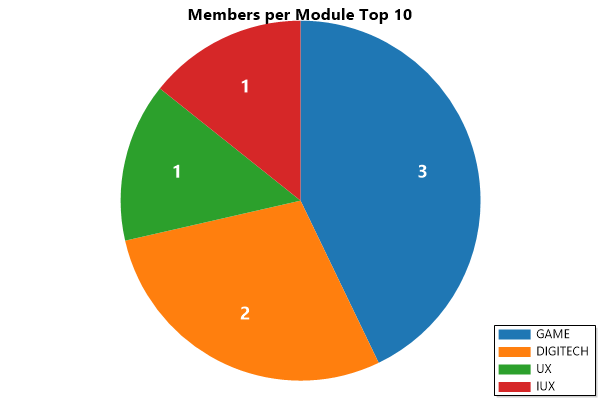
\includegraphics[width=0.7\textwidth]{img/membersPerModule.png}
    \caption{Members per module}
    \label{fig:members-per-module}
\end{figure}
\clearpage

\subsubsection{Logging}
Für ein sauberes Entwickeln und einen sauberen operativen Einsatz gehört das Schreiben von Log-Einträgen dazu. 
Damit man nachvollziehen kann, welche Schritte der Bot unternommen hat, sowie bei Fehlern schneller reagieren kann.\\
Als Logging Framework wurde sich für NLog entschieden.\autocite{noauthor_nlog_nodate}
Dies aus dem Grund, da es das verbreitetste Logging Framework für .Net Applikationen ist und es einfach in das Microsoft Logging System integriert werden kann. 
Auch ist es Open Source und kostenlos für die Nutzung. 
Für eine saubere Ausführung benötigt NLog eine Konfigurationsdatei. 
In dieser kann das Logging Format angegeben werden, die Dateien in welche geloggt werden soll, sowie allfällige Farbeinstellungen für verschiedene Log-Levels. 
Die NLog.config Datei für dieses Projekt sieht folgendermassen aus.

\begin{lstlisting}[language=XML]
<?xml version="1.0" encoding="utf-8" ?>
<nlog xmlns="http://www.nlog-project.org/schemas/NLog.xsd" xmlns:xsi="http://www.w3.org/2001/XMLSchema-instance">
    <targets>
        <target name="coloredConsole" xsi:type="ColoredConsole" useDefaultRowHighlightingRules="false"
        layout="${longdate}| ${pad:padding=5:inner=${level:uppercase=true}}| ${pad:padding=-50:inner=${logger}}| ${message:withexception=true}" >
            <highlight-word condition="level == LogLevel.Debug" foregroundColor="Gray" text="DEBUG"/>
            <highlight-word condition="level == LogLevel.Info" foregroundColor="Green" text="INFO" />
            <highlight-word condition="level == LogLevel.Warn" foregroundColor="Yellow" text="WARN" />
            <highlight-word condition="level == LogLevel.Error" foregroundColor="Red" text="ERROR"/>
            <highlight-word condition="level == LogLevel.Fatal" foregroundColor="Red" text="FATAL" backgroundColor="White" />
        </target>
    </targets>
    <rules>
        <logger name="*" minlevel="Debug" writeTo="coloredConsole" />
    </rules>
</nlog>
\end{lstlisting}

Es wird dabei entschieden, nur in die Konsole zu loggen. 
Da der Server, auf welchem der Bot läuft, wenn es gut läuft, nur einmal im Semester geöffnet werden muss, wird nicht unnötig Speicherplatz verbraucht. 
Die Log Daten kann man sich auch auf der Konsole anzeigen lassen.\\
Ein Log Eintrag sieht dabei wie folgt aus:

\begin{figure}[h]
    \centering
    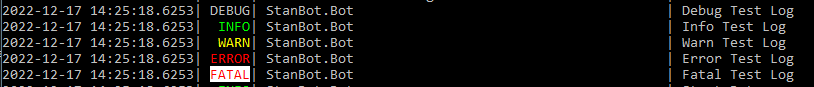
\includegraphics[width=1\textwidth]{img/LogLevels.png}
    \caption{Logging Beispiele}
    \label{fig:logging-examples}
\end{figure}

\newpage
\subsection{Sprint 5}
Im letzten Sprint wird eine Fehlermitteilung eingebaut, welche einen Admin bei einem Problem informiert. 
Auch wird der Bot startbereit gemacht, um ihn auf die produktive Umgebung zu deployen und ein Profilbild erstellt, welches ihn als Bot zu erkennen gibt.

\subsubsection{Stan Logo}
Damit der Bot ein sauberes Erscheinungsbild hat, wird für ihn ein Logo erstellt. 
Da Stan schon als Maskottchen von STAIR etabliert ist, nämlich als kleiner Kaktus, soll er noch mit einem spezifischen Discord Look ausgestattet werden.\\
Die Designs werden bei STAIR über die Plattform \textbf{Canva} verwaltet und erstellt. \autocite{noauthor_kostenloses_nodate}
Darin wird auch das Discord Stan Logo geboren.

\begin{figure}[h]
    \begin{minipage}[t]{0.5\textwidth}
        
\includegraphics[width=0.7\textwidth]{img/StanDiscordLogoSolo.png}
    \end{minipage}
    \begin{minipage}[t]{0.5\textwidth}
        
\includegraphics[width=0.7\textwidth]{img/StanDiscordLogo.png}
    \end{minipage}
    \caption{Stan Discord Logo}
    \label{fig:stan-discord-logo}
\end{figure}

Diese Bilder können nun als Profilbild des Bots dienen, sowie als Vermarktungslogo für den STAIR Discord.

\subsubsection{Fehler Mitteilung}
Falls während der Laufzeit Fehler auftreten, also aus irgendeinem Grund der E-Mail Service nicht mehr funktioniert, oder die Datenbank abstürzt, soll ein Administrator kontaktiert werden. 
Dieser Kontakt soll bei einem Datenbankabsturz über E-Mail erfolgen und bei einem E-Mail Service Absturz über eine private Nachricht auf Discord.\\
Damit der Administrator bei einem Absturz nicht mit Nachrichten und E-Mails überhäuft wird, wird derselbe Fehler maximal einmal alle 4 Stunden an den Administrator gesendet. 
Das heisst, er bekommt nur einmal die Nachricht eines Absturzes und erst, wenn er das Problem nach 4 Stunden nicht gelöst hat, bekommt er wieder eine Nachricht.
\newpage
Damit der Bot weiss, welche Personen als Administrator hinterlegt sind, wird in der Datenbank in der Studierendentabelle das Feld \textbf{IsDiscordAdmin} auf \textbf{True} gesetzt. 
Diese Zuweisung zum Discord Administrator kann per Command vorgenommen werden. 
Die Commands lauten:
\begin{itemize}
    \item \textbf{!addAdmin} <email-address>
    \item \textbf{!removeAdmin} <email-address>
\end{itemize}
Damit bei einem Datenbankabsturz die Administratoren, trotzdem noch ausgelesen werden können, werden diese E-Mail Adressen zusätzlich noch in eine Datei \textbf{discordAdmins.csv} gespeichert. 
Dies erfolgt auch bei der Ausführung der Commands.\\\\
In den Nachrichten werden folgende Informationen mitgegeben.
\begin{itemize}
    \item Die Art der Nachricht. Also ob es sich um einen Datenbank Fehler oder um einen Fehler des E-Mail Service handelt.
    \item Der Stacktrace der Exception.
    \item Die Message der Exception.
    \item Die Klasse, in welcher der Fehler geworfen wurde.
\end{itemize}
So eine Nachricht kann als E-Mail und als Discord Nachricht folgendermassen aussehen.
\begin{figure}[h]
    \begin{minipage}[t]{0.5\textwidth}
        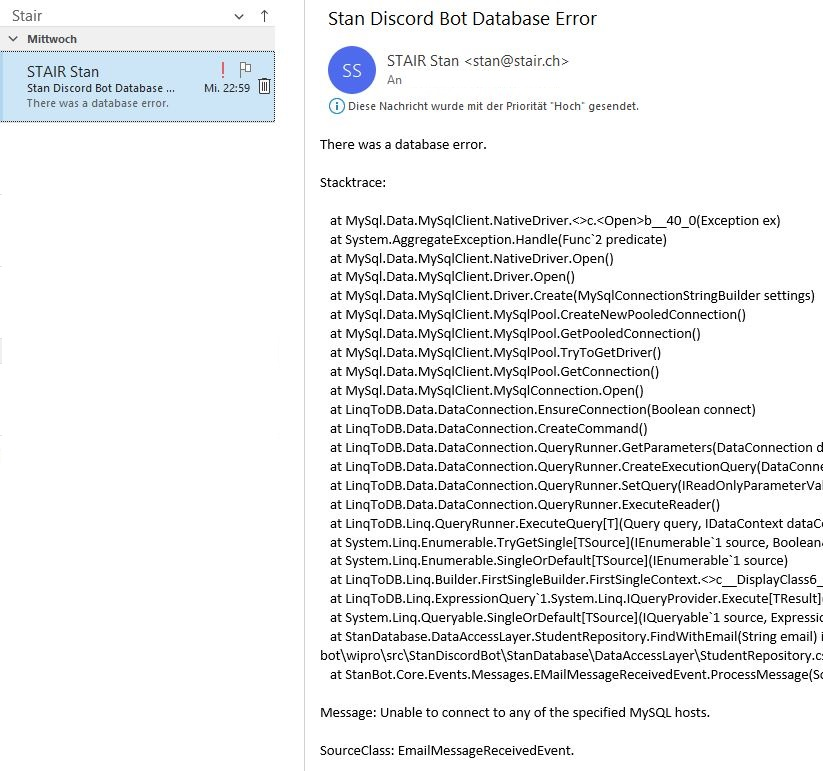
\includegraphics[width=1\textwidth]{img/DatabaseErrorNotificationEmail.png}
        \caption{Fehler Nachricht E-Mail}
    \end{minipage}
    \begin{minipage}[t]{0.5\textwidth}
        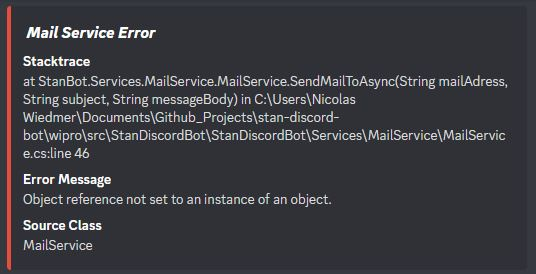
\includegraphics[width=1\textwidth]{img/MailErrorNotificationEmbed.png}
        \caption{Fehler Nachricht Discord}
    \end{minipage}
    \label{fig:error-notifications}
\end{figure}

\subsubsection{Bot als Deamon}
Der Discord Bot wird auf einem Linux Server des Enterprise Labs der Hochschule Luzern deployed. 
Dieser soll als Deamon laufen, also als Hintergrundservice des Servers. 
Mit diesem Vorgehen kann sichergestellt werden, dass der Service ununterbrochen läuft.\\
Um das Deployment auf Linux einfacher zu gestalten, bietet Microsoft eine systemd Bibliothek an, mit der der Host Provider in diese Umgebung eingefügt werden kann.\autocite{dotnet-bot_systemdhostbuilderextensionsusesystemdihostbuilder_nodate}
Dies kann mit folgendem Code hinzugefügt werden.

\begin{lstlisting}[language=csharp]
\\Program.cs
using IHost host = Host.CreateDefaultBuilder()
                .UseSystemd()
                .ConfigureServices((_, services) => services
                ...)
\end{lstlisting}

Die Bibliothek konfiguriert das Loggen in die Konsole im systemd-Format und stellt Benachrichtigungen beim Starten und Beenden der Anwendung bereit.

\newpage
\subsection{Testprotokolle Zusammenfassung}
Die manuellen Systemtests werden nach dem Drehbuch im Kapitel \nameref{Testdrehbuch} durchgeführt.
Der Bot ist zu diesem Zeitpunkt auf dem Linux Server deployed und wartet auf eintreffende Nachrichten. 
Die Mailservice Infrastruktur steht und ist bereit. 
Die Tests werden aber noch auf einem Discord Test Server durchgeführt. 
Der Bot wird erst nach dieser Arbeit in das laufende System eingebunden.\\\\
Im Folgenden wird eine Zusammenfassung der Testergebnisse aufgelistet. 
Die kompletten Testprotokolle können im Anhang im Kapitel \nameref{test-protocols} eingesehen werden.

\begin{table}[h]
    \centering
    \begin{tabular}{|l|p{30em}|}
        \hline
        \rowcolor[gray]{.9} Testfall & Erkenntnis \\
        \hline
        \#1 & Der Student bekommt direkt eine Nachricht. Keine Massnahmen nötig \\
        \hline
        \#2 & Der Authentifizierungsprozess funktioniert gut. Keine Massnahmen nötig. \\
        \hline
        \#3 & Nicht Studenten bekommen keinen Zugriff auf den Server. Keine Massnahmen nötig. \\
        \hline
        \#4 & Die Studenten werden richtig in das System eingelesen. Keine Massnahmen nötig. \\
        \hline
        \#5 & Die Module werden richtig in das System eingelesen. Keine Massnahmen nötig. \\
        \hline
        \#6 & 
            Der show <module> Command funktioniert richtig.
            Falls Module nicht gefunden werden wird eine Fehlermeldung vom Bot zurückgegeben.
            Diese könnte auch nach einiger Zeit gelöscht werden. \\
        \hline
        \#7 & 
            Der hide <module> Command funktioniert richtig.
            Falls Module nicht gefunden werden wird eine Fehlermeldung vom Bot zurückgegeben.
            Diese könnte auch nach einiger Zeit gelöscht werden. \\
        \hline
        \#8 & Es gibt 4 Statistic Commands. Diese funktionieren gut. Keine Massnahmen nötig. \\
        \hline
    \end{tabular}
    \caption{Testprotokoll - Erkenntnisse}
    \label{tab: test-protocol-knowledge}
\end{table}

\subsection{Einführung des neuen Bots}
Es wird gemeinsam mit dem Präsidenten von STAIR besprochen, dass das Einführen nicht in einem laufenden Semester oder während der Prüfungsphase stattfinden soll. 
So wird verhindert, dass bei einem auftauchenden Bug nicht den Studierenden die Austauschmöglichkeit des Discord Servers genommen wird.
Aus diesem Grund wird der Bot erst in den Blockwochen eingeführt.
Zu diesem Zeitpunkt ist der Austausch auf dem Server am kleinsten und die Neueinführung kann problemloser vonstatten gehen.

\newpage
\section{Evaluation und Validation}
Das Ziel dieser Arbeit war es, den Discord Bot des Studentenvereins STAIR neu zu implementieren, um die Administrationsarbeit auf dem Server zu verringern und neu Daten für Event- und Marketingplanung zu sammeln. 
Darauf wurde in dieser Arbeit hingearbeitet.\\
In der ersten Phase wurden Ideen und Konzepte zum Stand der Technik, sowie Methoden zur Projektdurchführung ausgearbeitet. 
Für dieses Projekt haben wir uns verstärkt mit den Sprach und Text-Messengern auf dem Markt auseinandergesetzt und diese Discord gegenübergestellt. 
Da im Vorfeld Discord als Zielplattform schon vorgegeben war, haben die anderen Plattformen nicht zu unserer Entscheidung beigetragen, Discord als Plattform zu wählen. 
Allerdings gab es uns die Möglichkeit andere Plattformen anzuschauen und diese vielleicht in zukünftige Umgestaltungen mit einzubeziehen.\\
Für die Projektmethode wurde die an der Hochschule praktizierte Softwareentwicklungsmethode, \gls{SoDa} ausgewählt. 
Durch das in Sprints aufgeilte Vorgehen in der SoDa Methode kann die Projektführung stark erleichtert werden.
Die User-Stories boten eine gute Möglichkeit, Softwarefeatures einfach zu definieren und zuzuteilen. 
Die Arbeit musste nicht auf das kleinste Paket heruntergebrochen werden, da eine User-Story alle Arbeitsschritte beinhaltete. 
Dadurch gestaltete die Arbeit angenehmer und machte die Planungsphase in einem nur 14-Wöchigen Projekt deutlich kürzer. 
Allerdings wurden die Anforderungen vor dem Projekt fix festgelegt und es sind während dem Projekt keine neuen Anforderungen hinzugekommen. 
Diese hätte man mit SoDa einfach in das Projekt eingliedern können, so wurde das Projekt aber sequentiell abgearbeitet.\\\\
In der Realisierungsphase wurde zuerst eine Analyse des alten Bots erstellt. 
Da der Bot veraltete .Net Versionen und Libraries verwendet hatte, wurde entschieden, einen neuen Bot zu implementieren, welcher beide vorherigen Bots vereint. 
Um das Ziel der Datensammlung zu erreichen, wurde im Hintergrund eine Datenbank eingeführt, welche die authentifizierten Studierenden mit den Discord Accounts verbindet. 
Auf dieser Datenbank wurde im Anschluss die Applikation aufgebaut.\\\\
Die neu implementierte Datenbank erhöhte die Administrationsarbeit auf der Serverseite. 
Dadurch, dass jedes Semester neue Studierende hinzukommen, sowie Module hinzugefügt oder gelöscht werden, muss die Datenbank auf dem neuesten Stand gehalten werden. 
Zu diesem Zweck wurde eine Bedienungsanleitung geschrieben, welche den Verlauf des Aktualisierens beschreibt. 
Auf der anderen Seite wurde der administrative Aufwand auf dem Discord Server erheblich reduziert, da Module nicht mehr manuell freigegeben werden müssen, und die beiden Bots jetzt zusammen laufen. 
Ausserdem werden mit den Daten neue Möglichkeiten eröffnet, um Event- und Marketingplanung zu betreiben.\\\\
Für uns und den Auftraggeber wurden die Ziele erreicht. 
Der neue Stan Bot bietet die gleichen und zusätzlichen Funktionen im Vergleich mit dem alten Bot. 
Damit kann der alte Bot abgelöst werden.

\newpage
\section{Ausblick}

Diese Projektarbeit hat uns sehr gefordert.
Der Aufbau einer neuen Softwarelösung ist nicht immer einfach und hält viele Tücken bereit.
Nichtsdestotrotz sind wir stolz auf unser Ergebnis und freuen uns, wenn das Produkt auf dem Discord Server im Februar 2023 live geht.\\
Doch auch wenn diese Arbeit jetzt abgeschlossen ist, gibt es Optimierungspotential und Visionen, welche in Zukunft aufgegriffen werden können.\\\\
Meherere dieser Visionen betreffen weitere Features.
Eine nächste Anforderung des STAIR Vorstandes an das Produkt könnte es sein, Unternehmungen oder Studierenden die Möglichkeit zu geben, direkt eigene Beiträge, wie beispielsweise Job Angebote oder Events auf Discord zu veröffentlichen.
Dies könnte anhand eines aufgeschalteten Formulares auf der STAIR Webseite geschehen.
Mithilfe des Discord Bots kann dieses Angebot verschickt und auf dem Discord Server veröffentlich werden.\\
In einem nächsten Schritt könnten die Haus-Punkte automatisiert im Discord Channel gepostet werden.
Momentan werden die Haus-Punkte innerhalb des Semesters gesammelt und müssen manuell nach jedem Event in den entsprechenden Discord Channel gepostete werden.\\
Verbesserungspotential besteht auch bei der Serverwahl.
Ein Communtiy Server wäre dem jetzigen privaten Server vorzuziehen, da bei der Verwendung des Community Servers einige neue Feautures und Pflichten implementiert werden können.
Dazu gehören beispielsweise Ankündigungskanäle, die es den Nutzern erlauben, Meldungen nach Bedarf ein- oder auszustellen.\autocite{noauthor_richte_nodate}\\\\
Im Grossen und Ganzen ist das Potential des STAIR Bots riesig.
Die Benutzerfreundlichkeit kann wie beschrieben, mithilfe des Bots weiter verbessert werden.
Die Grundsteine dafür sind gelegt.

\newpage
\section{Anh\"ange}

\subsection{Sprintreviews}\label{Sprintreviews}
In diesem Kapitel werden die einzelnen Sprintreviews aufgelistet.
Diese beinhalten immer eine Reflektion zum letzten Sprint mit einer Übersicht der umgesetzten User-Stories und
einer Retrospektive über aufgefallenen Problemen und dazugehörigen Massnahmen.

\subsubsection{Sprint 1}
\subsubsection*{Sprintziel}
Studentenerfassung ist implementiert.

\subsubsection*{Risiko-Update}
\begin{itemize}
    \item Kommunikation in Richtung Discord wurde im Vorfeld noch nicht bedacht.
    Kann sein das die Architektur angepasst werden muss, um Kommunikation ausgehend vom Bot starten zu können.
\end{itemize}

\subsubsection*{Sprintbacklog}
In diesem Sprint wurde nur eine User-Story umgesetzt.\\
\url{https://github.com/stairch/stan-discord-bot/issues/2}
\newline
Geschätzter Aufwand: 9 h
\newline
Effektiver Aufwand: 15 h\\
Die Abweichung fällt so hoch aus, da die User Story nur den Aspekt der Modullade-Funktionalität, abschätzt.
Die Datenbank musste in diesem Sprint aber auch noch erstellt werden, deshalb wurde mehr gearbeitet.

\subsubsection*{Retrospektive}
Erfolge:
\begin{itemize}
    \item LoadStudenten Script konnte einfach und schnell erstellt werden.
    \item Library Linq2db einfacher als erwartet.
\end{itemize}
Probleme:
\begin{itemize}
    \item Linq2db stellt keine Generierung der Datenbank aus den Klassen zur Verfügung.
\end{itemize}
Massnahmen:
\begin{itemize}
    \item Datenbank Schema muss manuell erstellt werden.
\end{itemize}
\newpage

\subsubsection{Sprint 2}
\subsubsection*{Sprintziel}
Modulerfassung ist implementiert und die Kommunikation mit Discord und dem Bot funktioniert.

\subsubsection*{Risiko-Update}
\begin{itemize}
    \item Keine.
\end{itemize}

\subsubsection*{Sprintbacklog}
In diesem Sprint wurden zwei User-Stories umgesetzt.\\
\url{https://github.com/stairch/stan-discord-bot/issues?q=is%3Aopen+is%3Aissue+milestone%3A%22Sprint+2%22}
\newline
Geschätzter Aufwand: 21 h
\newline
Effektiver Aufwand: 20 h

\subsubsection*{Retrospektive}
Erfolge:
\begin{itemize}
    \item Kommunikation mit Discord und dem Bot konnte sichergestellt werden.
    \item Ein Help und ein Ping Befehl konnten zum Testen implementiert werden.
    \item Der Bot schreibt einen Benutzer direkt an, sobald dieser den Server betritt.
    \item Die Modulerfassung alleine funktioniert.
\end{itemize}
Probleme:
\begin{itemize}
    \item Bei der Modulerfassung können die Kategorien noch nicht richtig erstellt werden und zugewiesen werden.
    Die ID der neu erstellten Kategorie wird nicht richtig zurückgegeben.
\end{itemize}
Massnahmen:
\begin{itemize}
    \item Kleines Test Projekt erstellen und weiter versuchen. Auf Logik-Fehler nochmal kontrollieren.
\end{itemize}
\newpage

\subsubsection{Sprint 3}
\subsubsection*{Sprintziel}
Der show/hide <module> Command wurde implementiert und der E-Mail versandt für das Authentifizieren.

\subsubsection*{Risiko-Update}
\begin{itemize}
    \item Die Modulerfassung funktioniert immer noch nicht.
    Prioritäten müssen gesetzt werden.
    Kann sein, dass sich Issues nach hinten verschieben.
\end{itemize}

\subsubsection*{Sprintbacklog}
In diesem Sprint wurden zwei User-Stories umgesetzt.\\
\url{https://github.com/stairch/stan-discord-bot/issues?q=is%3Aopen+is%3Aissue+milestone%3A%22Sprint+3%22}
\newline
Geschätzter Aufwand: 27 h
\newline
Effektiver Aufwand: 19 h\\
Beide User Stories wurden zu hoch eingeschätzt. 
Die Infrastruktur stand zu diesem Zeitpunkt schon.
Aus diesem Grund haben die beiden User-Stories nicht so lange gedauert, wie geschätzt.

\subsubsection*{Retrospektive}
Erfolge:
\begin{itemize}
    \item Der E-Mail Versand konnte implementiert werden und sollte funktionieren.
    Das Device, auf welchem der Bot läuft, wird beim Starten von dem Azure Dienst erkannt und kann hinzugefügt werden.
\end{itemize}
Probleme:
\begin{itemize}
    \item Der E-Mail versandt läuft über eine Azure Applikation, für die wir die Berechtigung noch nicht haben.
    Das Device kann somit noch nicht hinzugefügt werden.
    \item Die Modulerfassung funktioniert immer noch nicht.
    \item Mit dem show/hide <module> Issue wurde noch nicht begonnen.
\end{itemize}
Massnahmen:
\begin{itemize}
    \item Die Accountinfromationen für den Mail-Service einholen, damit die E-Mail Kommunikation getestet werden kann.
    \item Prioritäten setzten was die Modulerfassung anbelangt.
    \item Möglichst zeitnah mit dem neuen Issue beginnen.
\end{itemize}

\newpage
\subsubsection{Sprint 4}
\subsubsection*{Sprintziel}
Die Statistiken für die STAIR Mitglieder wurden implementiert, sowie ein stabiles Logging Framework.

\subsubsection*{Risiko-Update}
\begin{itemize}
    \item Durch das Hinzufügen immer mehr Libraries steigt die Wahrscheinlichkeit, dass es Probleme beim Deployen des Bots auf den Linux Server gibt.
\end{itemize}

\subsubsection*{Sprintbacklog}
In diesem Sprint wurde eine User-Story umgesetzt.\\
\url{https://github.com/stairch/stan-discord-bot/issues?q=is%3Aissue+milestone%3A%22Sprint+4%22+}
\newline
Geschätzter Aufwand: 9 h
\newline
Effektiver Aufwand: 8 h

\subsubsection*{Retrospektive}
Erfolge:
\begin{itemize}
    \item Das Problem der letzten beiden Sprints mit der Datenbank konnte gelöst werden.
    Dort wurde für die Erstellung von Models Konstruktoren eingesetzt.
    Diese wurden allerdings von Linq2DB nicht richtig aufgerufen, \gls{bzw.} befüllt.
    Aus diesem Grund haben wir die Konstruktoren weggelassen und eine statische CreateNew Methode hinzugefügt.
    \item Die Statistiken konnten erfolgreich implementiert werden.
    \item Es konnte ein stabiles Logging Framework NLog in das System eingebunden werden.
    \item Für den E-Mail Versand wurde der richtige Account von STAIR freigeschalten.
    Dieser kann jetzt erfolgreich genutzt werden.
    \item Der show und hide Command konnte erfolgreich umgesetzt werden.
\end{itemize}
Probleme:
\begin{itemize}
    \item Bei den Commands gibt es ein RequireRole Attribut, welches man eigentlich verwenden kann um die Rolle des Aufrufenden Benutzers zu prüfen.
    Dieses funktioniert allerdings nicht.
\end{itemize}
Massnahmen:
\begin{itemize}
    \item Es muss eine Alternative gesucht werden um die Berechtigung einzuholen.
    Man kann \gls{z.B.} nur von einem bestimmten Channel aus Commands versenden.
\end{itemize}

\newpage
\subsubsection{Sprint 5}
\subsubsection*{Sprintziel}
Die Fehlermeldung wurde im Bot integriert und der Startkonfiguration wurde systemd hinzugefügt.

\subsubsection*{Risiko-Update}
\begin{itemize}
    \item Keine.
\end{itemize}

\subsubsection*{Sprintbacklog}
In diesem Sprint wurde eine User-Story umgesetzt.\\
\url{https://github.com/stairch/stan-discord-bot/issues?q=is%3Aissue+milestone%3A%22Sprint+5%22+}
\newline
Geschätzter Aufwand: 5 h
\newline
Effektiver Aufwand: 5 h

\subsubsection*{Retrospektive}
Erfolge:
\begin{itemize}
    \item Die Fehlermitteilungen konnten erfolgreich hinzugefügt werden.
    \item Die systemd Konfiguration konnte hinzugefügt werden.
    \item Es wurde ein Stan Discord Logo designed und implementiert.
\end{itemize}
Probleme:
\begin{itemize}
    \item Bei immer mehr Klassen in der Dependency Injection, kann es zu Circular Dependencies kommen.
\end{itemize}
Massnahmen:
\begin{itemize}
    \item Dort Clean Coding Vorgehen anwenden. wo es Sinn macht.
    \item Bei immer mehr werdenden Klassen muss informiert werden, wie diese schön ins System injected werden können.
\end{itemize}

\newpage
\subsection{Arbeitsjournal Zusammenfassung}
Die Zeitvorgabe des Projektes bestand aus 180 Arbeitstunden für jede Person.
Für die User-Stories wurden gesamt 70 Stunden eingeplant, siehe Kapitel \nameref{user-stories}.
Dies bedeutet, dass noch 290 Stunden für Pitch, Projektmanagement und Dokumentation sowie Recherche zur Verfügung stehen.\\
Nach Abschluss des Projektes wurde folgende IST-Übersicht erstellt.

\begin{figure}[h]
    \centering
    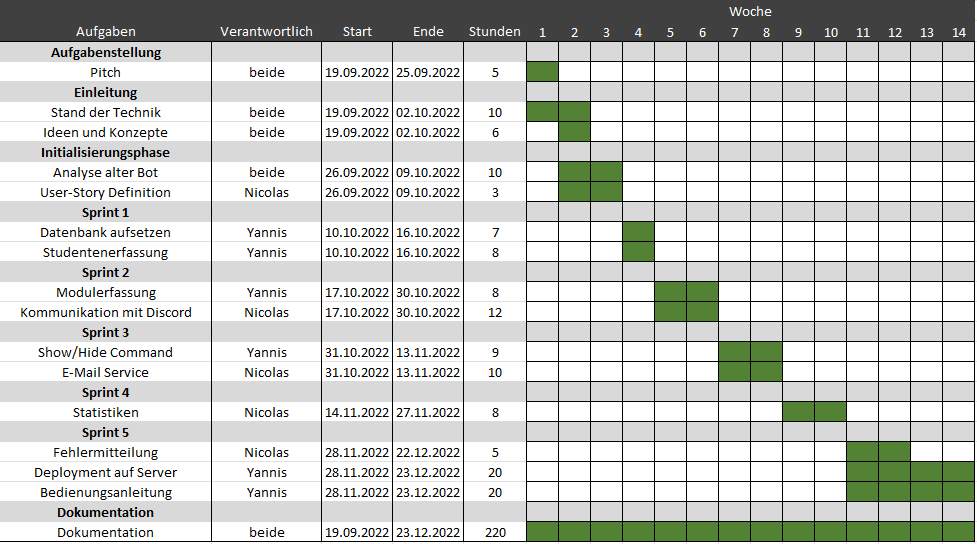
\includegraphics[width=1\textwidth]{img/Projektplan-IST.png}
    \caption{Projektplan IST-Zustand}
    \label{fig:plan-hours-actual-state}
\end{figure}

Eine genaue Übersicht der geleisteten Stunden findet man im Kapitel \nameref{work-journal-complete}.

\newpage
\subsection{Arbeitsjournal Komplett}\label{work-journal-complete}
Arbeitsjournal Nicolas Wiedmer.
Anzahl Stunden: 181.45

\begin{longtable}[h]{|l|l|l|p{20em}|l|}
    \hline
    \rowcolor[gray]{.9} Datum & Von & Bis & Tätigkeiten & Anz. Stunden  \\
    19.09.2022 & 13:00 & 14:30 & Aufsetzten einer Odnerstruktur in OneDrive. Nochmaliges durchlesen des Auftrags auf der Projektschiene. & 01:30 \\
    19.09.2022 & 15:00 & 16:00 & Erste Pitch Vorlage   vorbereiten. & 01:00  \\
    19.09.2022 & 19:30 & 21:00 & Besprechung mit Yannis. Erklärung der Aufgabe.   Freigabe aller Berechtigungen für die verschiedenen Plattformen & 01:30 \\
    20.09.2022 & 09:30 & 11:00 & Erstellen eines Logos für unseren Discord Bot & 01:30 \\
    21.09.2022 & 13:00 & 16:00 & Gemeinsames Arbeiten mit Yannis. Fertigstellung des   Pitchs. Klonen des jetzigen Repositories und installieren von Latex & 03:00 \\
    23.09.2022 & 17:00 & 18:15 & Kick-Off Meeting mit der Betreuungsperson & 01:15 \\
    27.09.2022 & 09:00 & 11:00 & Erstellen des Arbeitsjournal und Freigabe des   Ordners für Betreuungsperson. Einarbeitung in LaTeX und einfügen des   Deckblattes und der richtigen Titel & 02:00 \\
    27.09.2022 & 12:45 & 14:00 & Einrichten von Zotero und Verbinden mit Latex & 01:15 \\
    27.09.2022 & 14:00 & 16:00 & Recherche und schreiben über Discord & 02:00 \\
    28.09.2022 & 09:30 & 11:15 & Klassendiagramm vom derzeitigen StanBot erstellt & 01:45 \\
    28.09.2022 & 13:00 & 17:00 & Treffen mit Yannis. Ausarbeiten des ER-Diagramms   und besprechen allg. Punkte im Design des neuen Bots. & 04:00 \\
    30.09.2022 & 15:30 & 17:30 & Schreiben Doku. Aufbau   Discord & 02:00 \\
    03.10.2022 & 13:00 & 14:00 & Abschnitt Discord   überarbeitet & 01:00 \\
    04.10.2022 & 08:45 & 09:50 & Projekttypisierung & 01:05 \\
    04.10.2022 & 15:15 & 17:40 & Vorgehensmodell und   Rahmenplan beschrieben & 02:25  \\
    05.10.2022 & 13:00 & 15:00 & Treffen mit Yannis. Ausarbeiten der einzelnen   Projekte in der neuen Solution und definieren der Bilbiotheken. & 02:00 \\
    07.10.2022 & 15:30 & 18:30 & Doku Vorgehensmodell, Rahmenplan und Meilensteine   fertig beschreiben. Epics definieren & 03:00 \\
    11.10.2022 & 12:00 & 13:15 & User Stories angefangen zu dokumentieren & 01:15 \\
    11.10.2022 & 16:45 & 17:45 & Weiter User Stories und   in Latex longtables implementiert & 01:00 \\
    12.10.2022 & 09:30 & 10:20 & User Stories fertig   dokumentiert. & 00:50 \\
    12.10.2022 & 10:30 & 11:45 & Sprintplanung erstellt. Teststrategie und Vorlage   für die Sprintreview von Sprint 1 geschrieben. & 01:15 \\
    12.10.2022 & 13:15 & 15:00 & Treffen mit Yannis. Besprechung jetziger Stand. & 01:45 \\
    12.10.2022 & 16:00 & 19:10 & User-Stories in Github eingetragen und Zuweisungen   gemacht. Template für Testdrehbuch erstellt. Erste Testfälle geschrieben & 03:10 \\
    14.10.2022 & 15:25 & 16:05 & Besprechung mit Yannis und Herr Waldmann. & 00:40 \\
    17.10.2022 & 08:45 & 12:30 & Fertigstellen des Testdrehbuchs. Neu arrangieren   der Kapitel und Anfangen mit Risikomanagement. & 03:45 \\
    17.10.2022 & 14:45 & 16:00 & Risikotabellen & 01:15 \\
    17.10.2022 & 20:00 & 21:00 & Sprint 1 Review mit   Yannis & 01:00  \\
    19.10.2022 & 10:00 & 13:00 & Doku & 03:00  \\
    24.10.2022 & 13:15 & 16:30 & Discord Bot angefangen zu implementieren. User Story   Authentifizierung. & 03:15 \\
    24.10.2022 & 16:50 & 18:15 & Worker and Systemd angeschaut, um den Bot als   Deamon auf dem Linux Server laufen zu lassen. & 01:25 \\
    25.10.2022 & 13:00 & 17:00 & Versucht Bot richtig aufzusetzten mit Dependency   Injection und richtigem Config laden. & 04:00 \\
    26.10.2022 & 10:30 & 11:30 & Hinzufügen von Commands. Der Bot soll Chat   Nachrichten mitlesen um zu bestimmen, ob ihm Commands gesendet werden. & 01:00 \\
    26.10.2022 & 16:30 & 19:00 & Hinzufügen von Ping und Help Command. Versucht   die richtigen Berechtigungen für den Bot zu vergeben, im Zusammenspiel mit   den gateway Intents. & 02:30   \\
    26.10.2022 & 19:45 & 22:25 & Erstellen von einem Event Handler, bei dem alle   Discord Client Events registriert werden. Die Einzelnen Events werden in   Klassen separiert. Message Events allgemein, werden über einen Message   Handler vergeben und implementieren ein Message Receiver Interface. & 02:40 \\
    31.10.2022 & 08:30 & 10:45 & Korrektes weiterleiten der Nachrichten an den   richtigen Message receiver. Mithilfe von Regex und ChannelType überprüfung. & 02:15  \\
    31.10.2022 & 13:00 & 18:50 & Implementieren vom Repository Pattern für die   Datenbank. Umschreiben der LoadStudent und LoadModules Scripts. Einfügen der   Methoden zum Speichern der Daten während des Authentifikationsprozesses. & 05:50  \\
    02.11.2022 & 13:30 & 15:00 & Treffen mit Yannis. Besprechung jetziger Stand   und vorstellen der Implementierung. & 01:30  \\
    09.11.2022 & 08:15 & 12:00 & Verifizieren des Codes bei der Authentifikation   und Erstellen eines neuen Discord Accounts in der Datenbank, verlinkt mit dem   User. Danach auslesen der Rollen für den verlinkten Discord Account und   zuweisen der Rollen. & 03:45  \\
    09.11.2022 & 13:30 & 19:00 & Email-Service eingebunden. Dabei wurde der   gleiche verwendet, wie beim alten Bot, da dort schon ein funktionierendes   System läuft. & 05:30 \\
    14.11.2022 & 15:30 & 17:30 & Dokumentation Repository Pattern und Solution   aufsetzen & 02:00  \\
    14.11.2022 & 18:15 & 19:40 & Dokumentation. Hinzufügen von listings zum   Darstellen der Code snippets und erklären von Dependency Injection und   Services & 01:25 \\
    16.11.2022 & 13:10 & 15:30 & Doku und Besprechung mit Yannis & 02:20 \\
    16.11.2022 & 15:30 & 16:15 & Besprechung mit Herr   Waldmann & 00:45  \\
    23.11.2022 & 08:00 & 11:05 & Erstellen Prozessdiagramme für Modulanmeldung und   Authentifizierungsprozess & 03:05  \\
    23.11.2022 & 15:15 & 17:10 & Debugging Category class   und Datenbank & 01:55  \\
    24.11.2022 & 08:20 & 11:00 & Weiteres Debugging mit der Id und der Category   class. Funktioniert immer noch nicht. Beim ersten Insert geht es, aber nacher   gibt es 0 zurück & 02:40\\
    24.11.2022 & 15:00 & 16:00 & Weiter Debuggen. Hilfe von Tibo. Herausgefunden   das das falsche Auslesen am Konstruktor gelegen hat. & 01:00 \\
    25.11.2022 & 15:15 & 18:00 & Bugs gefixed. Verlinkung vom Discord Account zu   den Rollen gemacht und diese richtig asigned. & 02:45 \\
    26.11.2022 & 10:00 & 12:30 & Beim joinen vom Server wird im   Authentifizierungsprozess geprüft ob der User schon einmal auf dem Server   war. Dann wird ihm   einfach die Role zurückgegeben. & 02:30  \\
    29.11.2022 & 09:30 & 13:30 & Den ersten Statistic command implementiert. Kann   nun die Anzahl Studenten pro Haus abfragen & 04:00  \\
    29.11.2022 & 14:10 & 19:10 & Added 3 more statistical   methods to use from discord. & 05:00  \\
    02.12.2022 & 16:30 & 18:00 & Doku. Command Service   erklärt & 01:30 \\
    05.12.2022 & 10:30 & 12:15 & Doku. Risikomatrix vervollständigt. Kapitel   hinzugefügt & 01:45  \\
    05.12.2022 & 13:00 & 14:30 & ER-Diagramm erstellt. & 01:30  \\
    05.12.2022 & 16:30 & 17:30 & Message Handling   Klassendiagramm erstellt & 01:00 \\
    05.12.2022 & 18:15 & 20:30 & Hinzufügen der Diagramme in die Doku und   vervollständigen von Links in Zotero. & 02:15  \\
    06.12.2022 & 08:30 & 11:30 & Informiert über Microsoft   Identity & 03:00  \\
    06.12.2022 & 13:00 & 18:30 & Login für den Stan Microsoft Account bekommen.   Konnte die Active Directory anschauen und die E-Mail-Funktion ausprobieren.   Diese funktioniert. Weiter wurde das Kapitel mit den Statistiken in der Doku   beschrieben & 05:30  \\
    06.12.2022 & 22:00 & 22:40 & Stan logo Kapitel in Doku hinzugefügt & 00:40 \\
    07.12.2022 & 18:00 & 21:15 & Code von Update Command überarbeitet und schön   gemacht. & 03:15\\
    07.12.2022 & 22:40 & 00:00 & Test ubuntu server   aufgesetzt & 01:20  \\
    08.12.2022 & 00:00 & 01:30 & shared folder auf ubuntu server eingerichtet und   text console application versucht zu deployen & 01:30 \\
    14.12.2022 & 10:00 & 13:15 & Nlog für alles logging eingerichtet und eine   Config datei erstellt zum farbe loggen. & 03:15 \\
    14.12.2022 & 14:30 & 22:00 & Treffen mit Yannis und Besprechung weiteres   Vorgehen. Fehler mitteilung an eingetragenen Discord Admin implementiert. & 07:30  \\
    15.12.2022 & 14:30 & 17:30 & Dokumentation und Besprechung mit Martin zum Anschauen   der jetzigen Ergebnisse & 03:00  \\
    16.12.2022 & 12:30 & 16:30 & Doku Fehlermitteilung & 04:00 \\
    16.12.2022 & 21:30 & 24:00 & Doku alle Kapitel   überarbeiten & 02:30 \\
    17.12.2022 & 00:00 & 02:00 & Kapitel fertig schreiben und Fehlermitteilung im   Code weiter implementieren & 02:00 \\
    17.12.2022 & 13:00 & 15:00 & Logging Kapitel fertig geschrieben und   Literaturresearch Methode & 02:00 \\
    19.12.2022 & 07:30 & 09:30 & Dokumentation mit Word auf Schreibfehler   überprüft & 02:00 \\
    20.12.2022 & 10:00 & 12:00 & Abstract schreiben & 02:00  \\
    20.12.2022 & 13:15 & 22:30 & Testprotokolle geschrieben und den Code darauf   getestet. Musste noch ein paar Sachen anpassen. Alte Studenten als   Exstudenten markieren und alte Module löschen hat nicht funktioniert. Hat einfach alle   gelöscht. Weiter recherchiert zu OxyPlot & 09:15  \\
    21.12.2022 & 09:00 & 12:15 & Besprechung mit Herr Waldmann und einfügen Header   und deaktivieren von Statistic Commands & 03:15 \\
    21.12.2022 & 14:30 & 18:00 & Projektplan für IST Zustand erstellt.  Arbeitsjournal & 03:30 \\
    \hline
    \caption{Arbeitsjournal Nicolas Wiedmer}
    \label{tab:work-journal-nicolas}
\end{longtable}
\clearpage

Arbeitsjournal Yannis Krämer.
Anzahl Stunden: 182.75

\begin{longtable}[h]{|l|l|l|p{20em}|l|}
    \hline
    \rowcolor[gray]{.9} Datum & Von & Bis & Tätigkeiten & Anz. Stunden  \\
    18.09.2022 & 16:00 & 18:00 & Durchlesen von Auftrag, Anschauen von bisheriger   Umsetzung & 02:00 \\
    19.09.2022 & 19:30 & 22:00 & Besprechung mit Nicolas, Arbeiten an Pitch & 02:30 \\
    21.09.2022 & 13:00 & 16:00 & Gemeinsames Arbeiten mit Nicolas (online).   Besprechung und Überblick Projekt und bisherige Lösung & 03:00 \\
    21.09.2022 & 20:15 & 21:30 & Weiter arbeiten am Pitch, Üben des Pitch,   Organisation Meeting & 01:15 \\
    22.09.2022 & 08:00 & 12:00 & Änderung Design Pitch, Durchgehen Auftrag,   Nachschauen der bisher genützten Libraries, Latex Vorlage teilen, Ordner   Struktur im Repository einfügen & 04:00 \\
    22.09.2022 & 16:10 & 16:30 & Freigabe Windows Server & 00:20 \\
    23.09.2022 & 10:00 & 11:00 & Remote Desktop zu Windows Server auf Linux Laptop   aufsetzen & 01:00 \\
    23.09.2022 & 17:00 & 18:15 & Kick-Off Meeting & 01:15 \\
    28.09.2022 & 11:00 & 11:10 & Anschauen der Änderungen von Nicolas, Besprechung   mit Nicolas & 00:10 \\
    28.09.2022 & 13:00 & 17:00 & Treffen mit Nicolas. Ausarbeiten des ER-Diagramms   und besprechen allg. Punkte im Design des neuen Bots. & 04:00 \\
    29.09.2022 & 11:00 & 11:30 & Zotero installieren, Notizen von Besprechung   einfügen in Dokumentation & 00:30 \\
    04.10.2022 & 19:00 & 21:15 & Dokumetieren, Start Ablaufdiagramme der   bisherigen Lösung & 02:15 \\
    05.10.2022 & 11:45 & 12:45 & Fertigstellung Ablaufdiagramme der bisherigen   Lösung & 01:00 \\
    05.10.2022 & 13:00 & 15:00 & Treffen mit Nicolas. Ausarbeiten der einzelnen   Projekte in der neuen Solution und definieren der Bilbiotheken. & 02:00 \\
    05.09.2022 & 15:00 & 15:30 & Aufräumen des Meetingraumes, Bestellung Linux   Server im Enterprise Lab, Dokunentieren der Besprochenen Themen in Meeting & 00:30 \\
    07.09.2022 & 09:00 & 09:30 & E-Mails an Sekretariat schreiben für Studenten   und Modul Liste & 00:30 \\
    10.10.2022 & 19:30 & 22:15 & Start Programmierung der Datenbank, Mergen von   Dokumentation, Community Server einlesen & 02:45 \\
    11.10.2022 & 20:30 & 22:30 & Nachführen Arbeitsjournal, Einfügen von   automatischer Zeitdauerrechnung in Arbeitsjournal, hochladen von Code   Änderungen & 02:00 \\
    12.10.2022 & 07:30 & 08:10 & Dokumentieren & 00:40 \\
    12.10.2022 & 12:45 & 13:30 & Dokumentieren & 00:45 \\
    12.10.2022 & 14:00 & 18:00 & Besprechung mit Nicolas, Dokumentieren von   Vision, Vergleiche von Tools, Technologien & 04:00 \\
    13.10.2022 & 12:45 & 13:20 & Besprechung mit STAIR (Martin und Estefania) & 00:35 \\
    13.10.2022 & 14:30 & 16:30 & Überprüfung der Daten vom Sekretariat   (Modulliste, Studentenliste), überarbeitung von verschiedenen Kapitel   (Vision, Toolabgleich, Technologien) & 02:00 \\
    14.10.2022 & 15:25 & 16:05 & Besprechung mit Nicolas und Herr Waldmann, Mergen   von Dokumentation in Git & 00:40 \\
    14.10.2022 & 16:15 & 16:25 & Hinzufügen einer Spalte im Arbeitsjournal & 00:10 \\
    16.10.2022 & 14:00 & 18:30 & Datenbank implementieren & 04:30 \\
    17.10.2022 & 20:00 & 21:00 & Sprint 1 Review mit   Nicolas & 01:00 \\
    18.10.2022 & 19:45 & 20:35 & Datenbankanpassungen   vornehmen & 00:50 \\
    19.10.2022 & 06:55 & 07:45 & Datenbankanpassungen   vornehmen & 00:50 \\
    20.10.2022 & 08:00 & 09:15 & Log Library einfügen, Datenbank Unit Test Projekt   hinzufügen, DB anpassen & 01:15 \\
    21.10.2022 & 15:40 & 16:20 & Besprechung mit Estefania & 00:40 \\
    21.10.2022 & 16:30 & 17:00 & Server aufsetzen & 00:30 \\
    26.10.2022 & 07:42 & 08:03 & Format in Dokumentation   verbessern & 00:21 \\
    26.10.2022 & 13:17 & 17:02 & Dokumentation nachführen über Implementierung,   Start Bedienungsanleitung Server aufsetzen & 03:45 \\
    28.10.2022 & 09:40 & 10:45 & Datenbank SQL File   finalisieren & 01:05 \\
    02.11.2022 & 13:30 & 15:00 & Besprechung mit Nicolas. Austausch von   Umsetzungen der letzten Woche & 01:30 \\
    02.11.2022 & 15:10 & 17:00 & Implentieren von kleineren Besprochenen Details & 01:50 \\
    06.11.2022 & 20:00 & 23:10 & Refactorings um doppelten Code zu vermeiden,   kleinere Formatsprobleme lösen in den Scripts, Datenbank Verbindungsproblem   anfangen zu lösen & 03:10 \\
    07.11.2022 & 18:42 & 23:59 & Datenbank zum Laufen bringen, LoadStudents Script   testen und Probleme beheben, LoadModules angefangen zu testen, aber hat noch   offenen Bug, Startup Settings konfigurieren & 05:17 \\
    08.11.2022 & 07:05 & 08:55 & Refactorings in Zusammenhang mit der Datenbank   Verbindung & 01:50 \\
    08.11.2022 & 17:18 & 18:00 &  & 00:42 \\
    09.11.2022 & 12:45 & 16:15 & Datenbank Problem debugging (leider ohne Erfolg),   Kommunizieren mit Nicolas über bisherig erledigte Aufgaben, Installation auf   Laptop (bisher immer auf Desktop Zuhause gearbeitet) & 03:30 \\
    10.11.2022 & 09:55 & 12:10 & Austausch Kontakte bei STAIR, Refactorings, wie   umbenennungen, Config aus der Datei ermöglichen für StanDB, Logging erweitern & 02:15 \\
    13.11.2022 & 18:05 & 18:25 & Austausch mit Martin von STAIR über bisherigen   Vortschritt & 00:20 \\
    15.11.2022 & 18:20 & 23:54 & Nachführen Arbeitsjournal, hochladen von   bisherigen Änderungen, Debugging ID Problem, Logging vermehrt einfügen,   Refactorings & 05:34 \\
    16.11.2022 & 13:23 & 16:50 & Besprechung mit Nicolas und Herr Waldmann, & 03:27 \\
    17.11.2022 & 10:20 & 11:45 & Dokumentation weiter gearbeitet, Einfügen des   Besprechungsprotokolls & 01:25 \\
    20.11.2022 & 14:30 & 16:40 & Gestartet mit   UpdateModules und UpdateStudents Commands. & 02:10 \\
    22.11.2022 & 19:40 & 23:30 & Weiter gearbeitet an UpdateModules und   UpdateStudents Commands. & 03:50 \\
    23.11.2022 & 13:20 & 17:10 & Besprechung mit Nicolas, Testing von   UpdateModules und UpdateStudents, Refactoring von bestehendem Code & 03:50 \\
    27.11.2022 & 14:10 & 17:40 & Debugging von Errors, Erweiterung der   Bedienungsanleitung & 03:30 \\
    29.11.2022 & 18:45 & 23:59 & Nachdokumentieren verschiedener Features, Update   der Bedienungsanleitung & 05:14 \\
    30.11.2022 & 00:00 & 00:40 &  & 00:40 \\
    30.11.2022 & 06:30 & 06:50 & Fortschritt hochladen & 00:20 \\
    30.11.2022 & 13:00 & 18:10 & Starten mit der Show und Hide Befehle & 05:10 \\
    02.12.2022 & 15:15 & 17:50 &  & 02:35 \\
    06.12.2022 & 19:10 & 23:59 & Weiterentwicklung und Testing von Featuers, Show   Command fertig stellen & 04:49 \\
    07.12.2022 & 00:00 & 01:00 & Merge Branches von   Dokumentation & 01:00 \\
    07.12.2022 & 07:30 & 07:58 & Code Änderungen hochladen und mergen & 00:28 \\
    07.12.2022 & 13:20 & 16:20 & Dokumentieren & 03:00 \\
    13.12.2022 & 20:40 & 23:30 & Dependency Injection bei verschiedenen Befehlen   einfügen & 02:50 \\
    14.12.2022 & 06:52 & 07:05 & Hochladen von Änderungen & 00:13 \\
    14.12.2022 & 12:30 & 23:10 & TODOs in Dokumentation   durchgehen & 10:40 \\
    15.12.2022 & 15:05 & 18:55 & Protokolle von Besprechungen in Dokumentation   einfügen & 03:50 \\
    16.12.2022 & 22:15 & 23:59 & Dokumentation im Kapitel   5 erarbeiten & 01:44 \\
    17.12.2022 & 00:00 & 03:35 &  & 03:35 \\
    17.12.2022 & 12:42 & 17:24 & Dokumentation Kapitel 5 beenden, Mergen von  Änderungen in Git & 04:42 \\
    17.12.2022 & 18:15 & 23:55 & Deployment auf Linux Server als Service,   Erstellen der Bedienungsanleitung, Erstellung des Deploymentscripts & 05:40 \\
    18.12.2022 & 14:35 & 18:50 & Beenden der Installation und Setup von MySQL und   Datenbank & 04:15 \\
    20.12.2022 & 13:40 & 18:20 & Server Setup & 04:40 \\
    20.12.2022 & 19:50 & 22:15 &  & 02:25 \\
    21.12.2022 & 08:05 & 12:20 & Besprechung mit Herr Waldmann, Erstellen des   Contextdiagrams & 04:15 \\
    21.12.2022 & 13:15 & 14:15 &  & 01:00 \\
    22.12.2022 & 09:00 & 12:06 & Nachführen des   Arbeitsjournals & 03:06 \\
    22.12.2022 & 13:05 & 18:00 & Schreiben Ausblick & 04:55 \\
    \hline
    \caption{Arbeitsjournal Yannis Krämer}
    \label{tab:work-journal-yannis}
\end{longtable}

\subsection{Diagramme}\label{diagrams}
\begin{landscape}
    \begin{figure}[ht]
        \centering
        \hspace*{-5cm}
        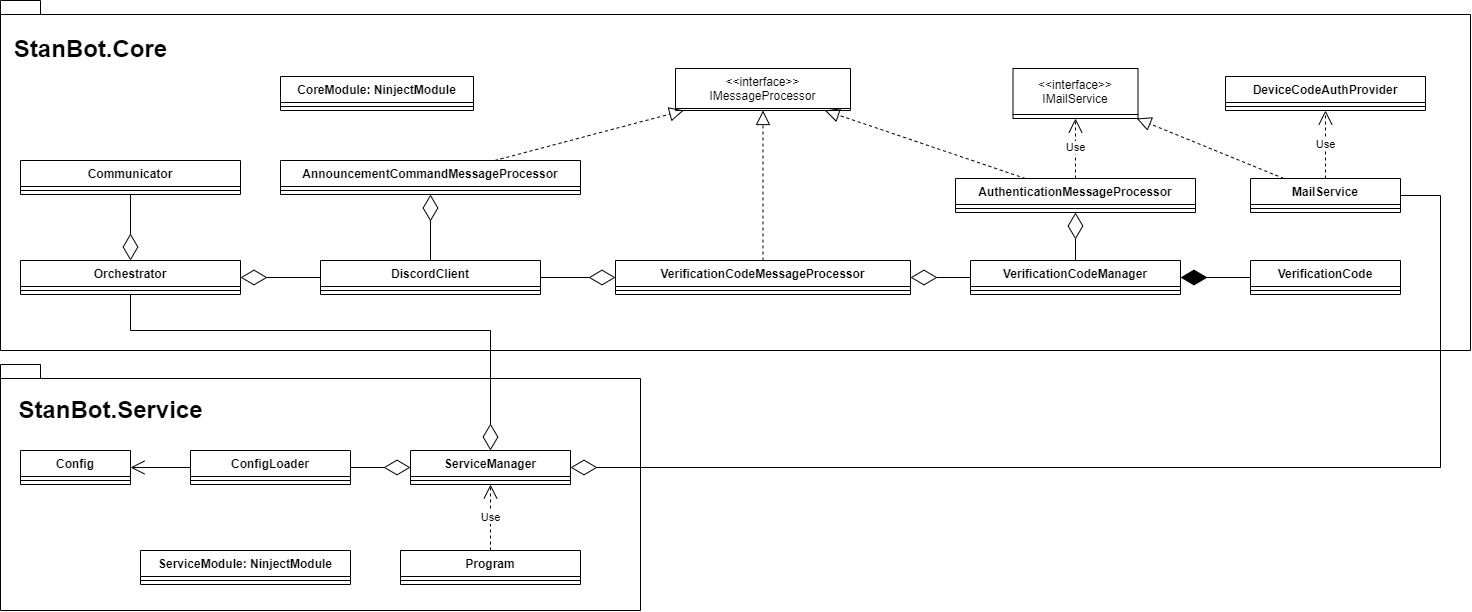
\includegraphics[width=1.7\textwidth]{img/Klassendiagramm_Bot_alt.png}
        \caption{Klassendiagramm Bot alt gross}
        \label{fig:Klassendiagramm_Bot_alt_big}
    \end{figure}
\end{landscape}

\begin{landscape}
    \begin{figure}[hb]
        \centering
        \hspace*{-4.5cm}
        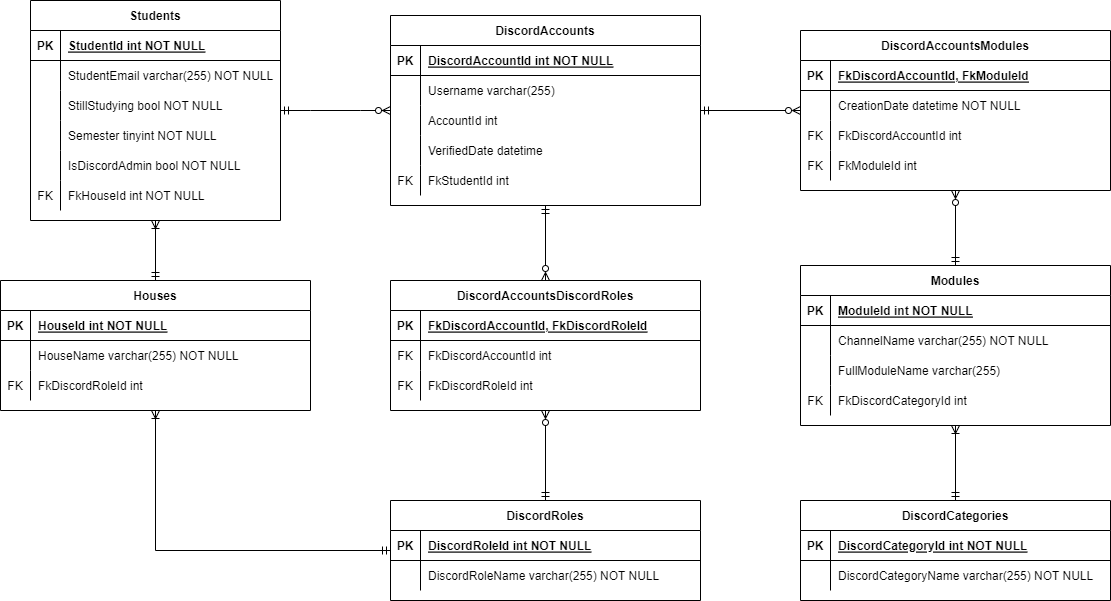
\includegraphics[width=1.6\textwidth]{img/ER-Diagramm.png}
        \caption{Entity Relationship Diagram Gross}
        \label{fig:ER-Diagram-big}
    \end{figure}
\end{landscape}

\begin{figure}[ht]
    \centering
    \hspace*{-2cm}
    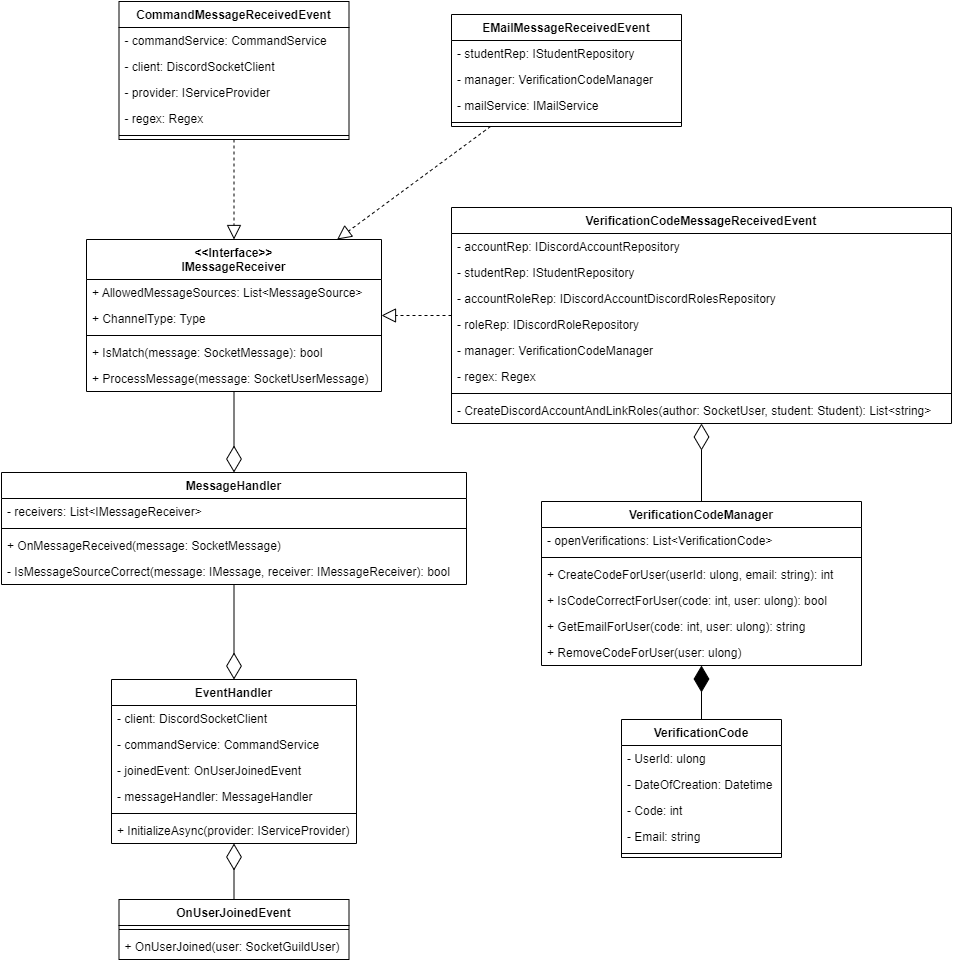
\includegraphics[width=1.3\textwidth]{img/MessageHandling.png}
    \caption{Message Handling}
    \label{fig:message-handling}
\end{figure}
\clearpage

\subsection{Testprotokolle}\label{test-protocols}
\begin{longtable}[h]{|p{9em}|p{31em}|}
    \hline
    \multicolumn{2}{|l|}{\textbf{Testfall \#1}} \\
    \hline
    \textbf{Titel} & Betritt ein neuer Student den Discord Server, bekommt er direkt eine Nachricht. \\
    \hline
    \textbf{Getestete Komponenten} & 
        \tabitem StanBot.OnUserJoinedEvent \\
    \hline
    \textbf{Tatsächliches Ergebnis/ Verhalten} & 
        Wenn ein neuer Besucher oder Besucherin auf den Server gelangt, erhält er/sie eine Direktnachricht vom Bot.
        In der Nachricht sind Informationen zum Anmeldeprozess sowie zu den Anstandsregeln beschrieben. \\
    \hline
    \textbf{Massnahmen} & Keine Massnahmen nötig. \\
    \hline
    \textbf{Datum} & 20.12.2022 \\
    \hline
    \textbf{Zusammenfassung} & 
        Es wird folgende Information dem Nutzer gesendet (der englische Teil wurde auf dem Bild weggelassen) 
        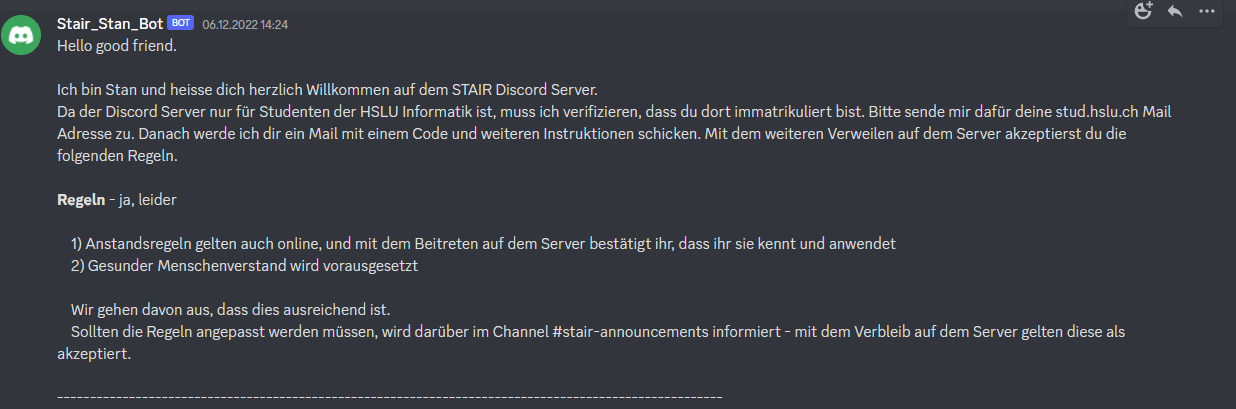
\includegraphics[width=0.8\textwidth]{img/Tests/1_Test_InfoMessage.png} \\
    \hline
    \caption{Testprotokoll - Testfall \#1}
\end{longtable}

\begin{longtable}[h]{|p{9em}|p{31em}|}
    \hline
    \multicolumn{2}{|l|}{\textbf{Testfall \#2}} \\
    \hline
    \textbf{Titel} & Ein Student kann sich beim Bot authentifizieren. Teil E-Mail. \\
    \hline
    \textbf{Getestete Komponenten} &  
        \tabitem StanBot.EMailMessageReceivedEvent \\*
     &  \tabitem StanBot.MailService \\*
     &  \tabitem Database \\
    \hline
    \textbf{Tatsächliches Ergebnis/ Verhalten} &  
        Der Student:in kann dem Bot seine korrekte E-Mail-Adresse schicken. 
        Der Bot kontrolliert in der Datenbank, ob der Student existiert und generiert einen zugehörigen Verifizierungscode.
        Im Anschluss wird korrekt eine E-Mail versendet mit dem Code sowie Instruktionen zum weiteren Vorgehen. \\
    \hline
    \textbf{Massnahmen} & Keine Massnahmen nötig.\\
    \hline
    \textbf{Datum} & 20.12.2022\\
    \hline
    \textbf{Zusammenfassung} & 
        Der Bot versendet erfolgreich diese Message. 
        
\includegraphics[width=0.8\textwidth]{img/Tests/2_Test_emailMessage.png} \\*
     &  Die Email: \\*
     &  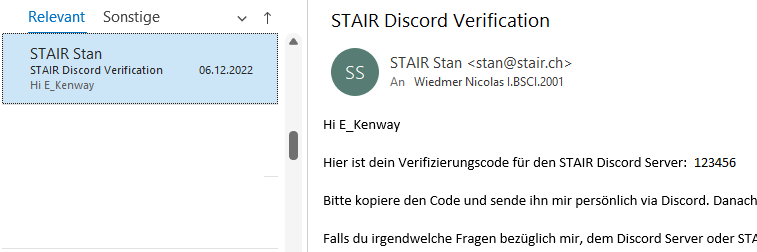
\includegraphics[width=0.8\textwidth]{img/Tests/2_Test_email.png} \\
    \hline
    \caption{Testprotokoll - Testfall \#2 E-Mail}
\end{longtable}

\begin{longtable}[h]{|p{9em}|p{31em}|}
    \hline
    \multicolumn{2}{|l|}{\textbf{Testfall \#2}} \\
    \hline
    \textbf{Titel} & Ein Student kann sich beim Bot authentifizieren. Teil Verifizierungscode. \\
    \hline
    \textbf{Getestete Komponenten} &  
        \tabitem StanBot.VerificationCodeMessageReceivedEvent \\*
     &  \tabitem Database \\
    \hline
    \textbf{Tatsächliches Ergebnis/ Verhalten} &  
        Wenn der Student erfolgreich die E-Mail vom Bot erhalten hat, kann er ihm den Authentifizierungscode per Discord senden. 
        Der Bot überprüft, ob der Student, der DiscordAccount und der Code übereinstimmen und erstellt in der Datenbank die Verlinkungen vom Studenten zum Discord Account. 
        Im Anschluss gibt er ihm die Studenten-Rolle sowie die zugehörige Haus Rolle frei. \\
    \hline
    \textbf{Massnahmen} & Keine Massnahmen nötig. \\
    \hline
    \textbf{Datum} & 20.12.2022 \\
    \hline
    \textbf{Zusammenfassung} & 
        Der Bot erstellt den Discord Account und die Verlinkungen in der Datenbank. 
        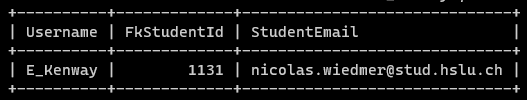
\includegraphics[width=0.8\textwidth]{img/Tests/2_Test_dbAccountStudent.png} \\*
      & 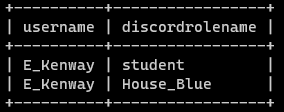
\includegraphics[width=0.4\textwidth]{img/Tests/2_Test_dbAccountRoles.png} \\*
      & Der Bot gibt erfolgreich die Rollen "student" und "House xy" frei. 
        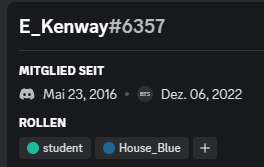
\includegraphics[width=0.3\textwidth]{img/Tests/2_Test_discordRole.png} \\
    \hline
    \caption{Testprotokoll - Testfall \#2 Verifizierungscode}
\end{longtable}

\begin{longtable}[h]{|p{9em}|p{31em}|}
    \hline
    \multicolumn{2}{|l|}{\textbf{Testfall \#3}} \\
    \hline
    \textbf{Titel} & Ein Nicht-Student kann sich nicht authentifizieren. \\
    \hline
    \textbf{Getestete Komponenten} &  \tabitem StanBot.EMailMessageReceivedEvent \\
    \hline
    \textbf{Tatsächliches Ergebnis/ Verhalten} & 
        Der Bot filtert alle Nachrichten heraus, die nicht dem Muster @stud.hslu.ch oder @hslu.ch entsprechen.
        Dies bedeutet aber auch, dass er keine Antwort gibt, falls Nachrichten nicht diesem Muster entsprechen.
        Falls Name oder Vorname nicht korrekt sind, erhält der Benutzer:in eine Nachricht, dass der Student:in nicht existiert. \\
    \hline
    \textbf{Massnahmen} & 
        Das keine Antwort zurückkommt kann verwirrend wirken. 
        Eventuell bei Direktnachrichten immer etwas zurückschreiben, wie \gls{z.B.} «Diesen Text habe ich nicht verstanden». \\
    \hline
    \textbf{Datum} & 20.12.2022\\
    \hline
    \textbf{Zusammenfassung} & 
        Nachricht, falls Student nicht existiert \\*
     &  
\includegraphics[width=0.6\textwidth]{img/Tests/3_Test_StudentNotFound.png} \\
    \hline
    \caption{Testprotokoll - Testfall \#3}
\end{longtable}

\begin{longtable}[h]{|p{9em}|p{31em}|}
    \hline
    \multicolumn{2}{|l|}{\textbf{Testfall \#4}} \\
    \hline
    \textbf{Titel} & Ein STAIR Administrator kann eine Liste mit Studenten in das System einlesen. \\
    \hline
    \textbf{Getestete Komponenten} & 
        \tabitem StanScripts.LoadStudents \\*
     &  \tabitem Database \\
    \hline
    \textbf{Tatsächliches Ergebnis/ Verhalten} &  
        Beim Ausführen des Scripts werden die richtigen Spalten extrahiert und geprüft. 
        Ist die \gls{CSV}-Datei korrekt, werden die neuen Studenten der Datenbank hinzugefügt und bei bestehenden Studenten das Semester aktualisiert.
        Am Schluss kann noch die Option ausgewählt werde, dass Studenten, welche nicht mehr auf der Liste vorhanden sind, als Ex-Studenten markiert werden. 
        Damit wird in der Datenbank das StillStudying Feld des Studenten auf False gesetzt. \\
    \hline
    \textbf{Massnahmen} & Keine Massnahmen nötig \\
    \hline
    \textbf{Datum} & 20.12.2022\\
    \hline
    \textbf{Zusammenfassung} & LoadStudent Script Output: \\*
     & 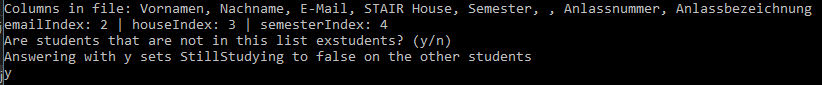
\includegraphics[width=0.8\textwidth]{img/Tests/4_Test_LoadStudents.png} \\
    \hline
    \caption{Testprotokoll - Testfall \#4}
\end{longtable}

\begin{longtable}[h]{|p{9em}|p{31em}|}
    \hline
    \multicolumn{2}{|l|}{\textbf{Testfall \#5}} \\
    \hline
    \textbf{Titel} & Ein STAIR Administrator kann eine Liste mit Modulen in das System einlesen. \\
    \hline
    \textbf{Getestete Komponenten} &  
        \tabitem StanScripts.LoadModules \\*
     &  \tabitem Database \\
    \hline
    \textbf{Tatsächliches Ergebnis/ Verhalten} &  
        Beim Ausführen des Scripts wird das \gls{CSV}-File auf korrekte Spalten überprüft und einigen Tests unterzogen. 
        Dabei wird geschaut, dass die Modulnamen und Nummern richtig extrahiert werden. 
        Den Modulen wird nun eine Category zugeordnet und in die Datenbank eingefügt. 
        Auch hier gibt es eine Option um Module, welche nicht mehr in der Liste vorhanden sind zu löschen. \\
    \hline
    \textbf{Massnahmen} & Keine Massnahmen nötig\\
    \hline
    \textbf{Datum} & 20.12.2022\\
    \hline
    \textbf{Zusammenfassung} & LoadModules Script Output \\*
     &  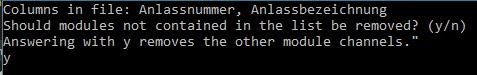
\includegraphics[width=0.8\textwidth]{img/Tests/5_Test_LoadModules.png} \\
    \hline
    \caption{Testprotokoll - Testfall \#5}
\end{longtable}

\begin{longtable}[h]{|p{9em}|p{31em}|}
    \hline
    \multicolumn{2}{|l|}{\textbf{Testfall \#6}} \\
    \hline
    \textbf{Titel} & Ein Student kann sich beim Bot für ein Modul anmelden. \\
    \hline
    \textbf{Getestete Komponenten} &  
        \tabitem StanBot.showCommand \\*
     &  \tabitem Database \\
    \hline
    \textbf{Tatsächliches Ergebnis/ Verhalten} & 
        Ein authentifizierter Student kann im Channel \#registering den show <module> Command ausführen.
        Falls das Modul nicht gefunden wurde, meldet es das zurück.
        Wenn das Modul gefunden wurde, wird der Discord Account mit dem Modul verlinkt und der Student als Mitglied dem Channel hinzugefügt. 
        Die Nachricht wird nach 5 Sekunden aus dem Chat gelöscht. \\
    \hline
    \textbf{Massnahmen} & Nachrichten von Modulen, welche nicht gefunden werden, könnten auch nach einer gewissen Zeit gelöscht werden. \\
    \hline
    \textbf{Datum} & 20.12.2022\\
    \hline
    \textbf{Zusammenfassung} & 
        Show command \\*
     &  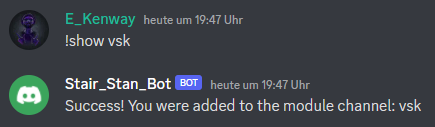
\includegraphics[width=0.6\textwidth]{img/Tests/6_Test_ShowCommandMessage.png} \\*
     &  Datenbankeintrag \\*
     &  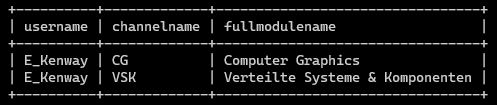
\includegraphics[width=0.6\textwidth]{img/Tests/6_Test_ShowCommandDatabase.png} \\
    \hline
    \caption{Testprotokoll - Testfall \#6}
\end{longtable}

\begin{longtable}[h]{|p{9em}|p{31em}|}
    \hline
    \multicolumn{2}{|l|}{\textbf{Testfall \#7}} \\
    \hline
    \textbf{Titel} & Ein Student kann sich beim Bot bei einem Modul abmelden. \\
    \hline
    \textbf{Getestete Komponenten} & 
        \tabitem StanBot.HideCommand \\*
     &  \tabitem Database \\
    \hline
    \textbf{Tatsächliches Ergebnis/ Verhalten} & 
        Wenn der Student den hide <module> Command in den \#registering Channel eingibt, wird er als Mitglied vom Channel entfernt. 
        Dadurch ist er für ihn nicht mehr sichtbar.
        Die Verlinkung in der Datenbank zwischen dem Discord Account und dem Modul wird aufgehoben.
        Die Nachricht wird auch nach 5 Sekunden aus dem Chat gelöscht. \\
    \hline
    \textbf{Massnahmen} & Nachrichten von Modulen, welche nicht gefunden werden, könnten auch nach einer gewissen Zeit gelöscht werden. \\
    \hline
    \textbf{Datum} & 20.12.2022\\
    \hline
    \textbf{Zusammenfassung} & 
        Hide command \\*
    &  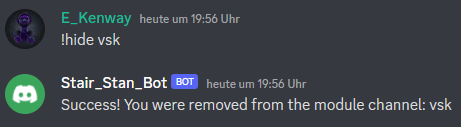
\includegraphics[width=0.6\textwidth]{img/Tests/7_Test_HideCommandMessage.png} \\*
    &  Datenbankeintrag \\*
    &  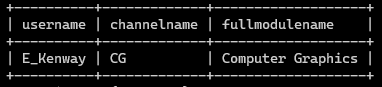
\includegraphics[width=0.5\textwidth]{img/Tests/7_Test_HideCommandDatabase.png} \\
    \hline
    \caption{Testprotokoll - Testfall \#7}
\end{longtable}

\begin{longtable}[h]{|p{9em}|p{31em}|}
    \hline
    \multicolumn{2}{|l|}{\textbf{Testfall \#8}} \\
    \hline
    \textbf{Titel} & Ein STAIR Administrator kann über eine Schnittstelle Statistiken auslesen. \\
    \hline
    \textbf{Getestete Komponenten} & 
        \tabitem StanBot.StatisticCommands \\ *
     &  \tabitem Database \\
    \hline
    \textbf{Tatsächliches Ergebnis/ Verhalten} & 
        Das STAIR Mitglied kann sich in Discord über den !help Command die verschiedenen Statistik Commands anzeigen lassen. 
        Wenn er einen ausführt, bekommt er die Statistik als Plot präsentiert. \\
    \hline
    \textbf{Massnahmen} & Keine Massnahmen nötig\\
    \hline
    \textbf{Datum} & 20.12.2022\\
    \hline
    \textbf{Zusammenfassung} & 
        Der studentsPerSemester Command \\*
     &  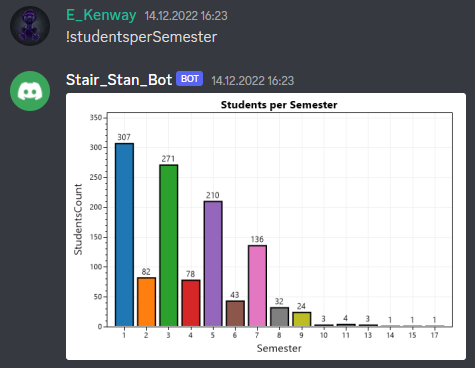
\includegraphics[width=0.7\textwidth]{img/Tests/8_Test_statisticCommand.png} \\
    \hline
    \caption{Testprotokoll - Testfall \#8}
\end{longtable}

\newpage
\section{Abbildungsverzeichnis}
\listoffigures

Nicht-referenzierte Grafiken sind Eigenproduktionen.

\section{Tabellenverzeichnis}
\listoftables

\section{Literaturverzeichnis}
\printbibliography

\newpage
\section{Bedienungsanleitung}\label{Bedienungsanleitung}

\subsection{Aufsetzen des Servers}

Der Stan Discord Bot kann auf verschiedenen Betriebssystemen genützt werden.
In dieser Anleitung wird jedoch auf das Aufsetzen für Ubuntu Linux 20.04 fokusiert.
Die Befehle müssen ebenfalls von einem Linux Computer in einer Bash-Konsole ausgeführt werden.
Mit \textit{Windows Subsystem for Linux (WSL)} sollte es jedoch auch funktionieren.

\begin{enumerate}
    \item Verbinde dich mit dem VPN oder verbinde dich mit dem WLAN der Hochschule Luzern
    \item Clone die beiden GitHub Repositories
        \begin{lstlisting}
            $ git clone https://github.com/stairch/stan-discord-bot.git
            $ git clone https://github.com/stairch/stair-config.git
        \end{lstlisting}
        \begin{enumerate}
            \item Achtung: Die beiden Repositories müssen im gleichen Überordner abgelegt sein, damit das \textit{buildAndDeploy} Script die Konfigurationsdateien findet kann.
        \end{enumerate}
    \item Verbinde dich mit dem Server über SSH
        \begin{lstlisting}
            $ ssh localadmin@stair-bot-lnx.el.eee.intern
        \end{lstlisting}
    \item Führe Updates durch
        \begin{lstlisting}
            # sudo apt update
            $ apt list --upgradablex
            # sudo apt upgrade -y
            # sudo apt autoremove
        \end{lstlisting}
    \item Installiere .NET 6
        \begin{lstlisting}
            # wget https://packages.microsoft.com/config/ubuntu/20.04/ packages-microsoft-prod.deb -O packages-microsoft-prod.deb
            # sudo dpkg -i packages-microsoft-prod.deb
            $ rm packages-microsoft-prod.deb
            # sudo apt update
            # sudo apt install -y dotnet-sdk-6.0
        \end{lstlisting}
    \item Lade den Code auf den Server
        \begin{lstlisting}
            # exit # Verlasse den Server
            $ cd /path/to/stan-discord-bot/wipro/src/
            $ sh buildAndDeploy.sh
        \end{lstlisting}
    \item Setze den StanBot als Service auf
        \begin{lstlisting}
            $ ssh localadmin@stair-bot-lnx.el.eee.intern
            # sudo cp ~/stan-discord-bot/wipro/src/stanBot.service /etc/systemd/system/
            # sudo systemctl daemon-reload # Konfigurationen neu laden
            # sudo systemctl start stanBot
            # sudo systemctl enable stanBot
            # sudo systemctl status stanBot
            # sudo journalctl -u stanBot -e # when there are problems
        \end{lstlisting}
    \item Installiere MySQL
        \begin{lstlisting}
            # sudo apt install mysql-server
            # sudo systemctl start mysql.service
            # sudo systemctl enable mysql.service
            # sudo systemctl status mysql.service
        \end{lstlisting}
    \item Setze MySQL auf
        \begin{lstlisting}
            # sudo mysql
            > # ersetze im folgenden Befehl "myPassword" mit dem neuen Passwort
            > ALTER USER 'root'@'localhost' IDENTIFIED WITH mysql_native_password BY 'myPassword';
            > exit
            $ mysql_secure_installation
            > -- folge den Fragen und antworte mit Y oder N
            Reload privilege tables now? : Y
            $ # Teste ob das neue Login funktioniert
            $ mysql -u root -p
            $ # Gebe das neu gesetzte Passwort ein
            > exit
            $ # Erstelle nun den Datenbank User fuer die Anwendung
            $ # Dieser muss mit dem Config File uebereinstimmen
            # sudo mysql
            > # ersetze im folgenden Befehl "myPassword" mit dem neuen Passwort
            > CREATE USER 'stanDbAcc'@'localhost' IDENTIFIED BY 'myPassword';
            > GRANT ALL PRIVILEGES ON StanDB.* TO 'stanDbAcc'@'localhost' WITH GRANT OPTION;
            > FLUSH PRIVILEGES;
            > exit
            $ Teste den neuen User
            # sudo mysqladmin -p -u stanDbAcc version
            $ # Es sollte nun die Version und andere Informationen angezeigt werden.
        \end{lstlisting}
    \item Erstelle die Datenbank
        \begin{lstlisting}
            $ mysql --host=localhost -u stanDbAcc -p < ~/stan-discord-bot/wipro/src/StanDatabase.sql
            $ exit # verlasse den Server
        \end{lstlisting}
    \item Es existiert ein Nutzer (E-Mail: info@stair.ch) auf Discord, welcher als StanBot fungiert. Das Passwort kann in der KeePass Datei gefunden werden.
    \item Füge den Bot Discord Account dem Discord Server hinzu.
        \begin{enumerate}
            \item Öffne die \href{https://discord.com/developers/applications} Seite des STAIR StanBot Accounts.
            \item Wähle den StanBot an.
            \item Gehe zum \textit{OAuth2} Tab
            \item Gebe dem Bot die folgenden Berechtigungen\par
                \begin{minipage}{\linewidth}
                    \centering
                    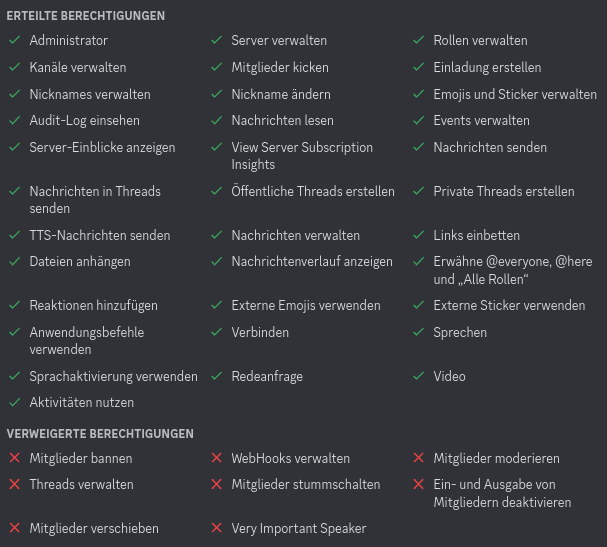
\includegraphics[width=1\textwidth]{img/berechtigungenBot.png}
                    %\caption{Anleitung - Berechtigungen Bot}
                    \label{fig:berechtigungenBot}
                \end{minipage}
            \item Die generierte URL kann nun genutzt werden um den Bot auf einen neuen Server einzuladen.
            \item Füge die URL im Browser ein.
            \item Wähle den Server, wo der Bot hinzugefügt werden soll. Hierfür werden Admin Rechte auf dem jeweiligen Discord Server benötigt.
        \end{enumerate}
    \item Teste den Bot mit den verschiedenen Befehlen
        \begin{enumerate}
            \item Für eine Übersicht von allen verfügbaren Befehlen steht der Befehl \textit{!help} verwendet werden.
        \end{enumerate}
    \item Admins registrieren
        \begin{enumerate}
            \item Öffne Discord
            \item Schicke im \textit{bot-commands} den Befehl \textit{!addAdmin <email-address>} für alle Administratoren des Discord Bots.
        \end{enumerate}
\end{enumerate}
Diese Anleitung baut auf folgenden Anleitungen auf:
\begin{enumerate}
    \item \href{https://devblogs.microsoft.com/dotnet/net-core-and-systemd/}{Systemd Service mit Dotnet erstellen}
    \item \href{https://blog.maartenballiauw.be/post/2021/05/25/running-a-net-application-as-a-service-on-linux-with-systemd.html}{Systemd Service mit Dotnet erstellen 2}
    \item \href{https://www.digitalocean.com/community/tutorials/how-to-install-mysql-on-ubuntu-20-04}{MySQL auf Ubuntu installieren}
    \item \href{https://askubuntu.com/questions/1004853/systemd-is-hanging-when-i-start-or-restart-a-service}{Systemd Service Konfiguration}
\end{enumerate}

\subsection{Konfiguration des StanBots}\label{konfigurationStanBot}

Die Settings Datei heisst \textit{stan.json}
\begin{lstlisting}[language=json]
{
    "DisordApplicationToken": "XXXX-XXXXX-XXXXXXXXXXXX",
    "Prefix": "!",
    "GuildId": "1234567891234567",
    "FromEmailAddress": "stan@stair.ch",
    "FromEmailName: "STAN",
    "AppId": "XXXXXXXX-XXXX-XXXX-XXXX-XXXXXXXX",
    "Scopes" ["Mail.Send", "Mail.Send.Shared"],
}
\end{lstlisting}

\subsection{Konfiguration der Datenbankverbindung}

Die zweite Konfigurationsdatei dient zur Datenbankverbindung,
sowie die Spezifikation der zu ladenden CSV Dateien.
Die Datei muss als \textit{stanDatabaseConfig.json} benannt sein und wird vom Stan Bot, sowie vom Stan Scripts verwendet.

\begin{lstlisting}[language=json]
{
    // database configuration
    "DatabaseName": "StanDB",
    "ConnectionString": "Server=localhost;Port=3306;Database=StanDB;Uid=stanDbAcc; Pwd=XXXXXXXXX;charset=utf8;",
    // csv configuration
    "Separator": ",",
    "EmailColumnNameInCsv": "E-Mail",
    "HouseColumnNameInCsv": "STAIR House",
    "SemesterColumnNameInCsv": "Semester",
    "ModuleShortnameColumnNameInCsv": "Anlassnummer",
    "ModuleFullnameColumnNameInCsv": "Anlassbezeichnung"
}
\end{lstlisting}

\newpage
\subsection{Instandhaltung Stan Discord Bot}

Der STAIR-Vorstand muss in regelmässigen Abständen die Hilfs-Channel auf dem Discord Server überwachen um zeitnah den Studierenden helfen zu können.
Ansonsten gibt es noch weitere Tasks, welche in den folgenden drei Kapitel genauer erklärt werden.

\subsubsection{Aktualisieren des Servers}

Der Server sollte in regelmässigen Abständen aktualisiert werden um keine Sicherheitslücken offen zu lassen.
Hierzu können die folgenden Befehle genützt werden:

\begin{lstlisting}
    # sudo apt update
    $ apt list --upgradable
    # sudo apt upgrade -y
\end{lstlisting}

\subsubsection{Aktualisieren der Module}

Um die Module zu aktualisieren, braucht man die aktuelle Liste der Module.
Diese kann ganz einfach beim Sekretariat der HSLU Informatik beantragt werden.
Bei der Modulliste ist zu beachten, dass alle Module in der Liste enthalten sein müssen, auch wenn sie dieses Semester nicht durchgeführt werden.
Ansonsten werden bisherige Chatverläufe von Modulen gelöscht, auch wenn diese ein Semester später erneut durchgeführt werden.
Die Liste wird im CSV Format benötigt.
Die Spaltennamen können in der Config-Datei von Stan Database festgelegt werden.
Hier ist ein Beispiel der einzulesenden Datei:

\begin{lstlisting}
    Anlassnummer,Anlassbezeichnung
    I.BA_111_DIGITECH.16,DI_Digital Technologies Fundamentals
    I.BA_112_UX.16,DI_User Experience Design & Engineering
    I.BA_113_GAME.20,DI_Game Design & Engineering
    I.BA_120_IUX.22,User Experience Design & Engineering
    I.BA_121_IGAME.22,Game Design & Engineering
\end{lstlisting}
Sobald diese Datei richtig formatiert wurde, kann diese über die Konsole eingelesen werden.
\begin{lstlisting}
    $ ssh localadmin@stair-bot-lnx.el.eee.intern
    $ mkdir \~/data # erstelle den Datenordner (muss nur beim ersten Mal ausgefuehrt werden)
    $ exit \# Server verlassen
    $ \# Dateinamen ersetzen durch die Datei welche hochgeladen werden sollte.
    $ scp ./ListeModuleDepI.csv localadmin@stair-bot-lnx.el.eee.intern:~/data/
    $ ssh localadmin@stair-bot-lnx.el.eee.intern
    $ cd /home/localadmin/stan-discord-bot/wipro/src/StanDiscordBot/artifacts/
    $ ./StanScripts.dll loadModules /home/localadmin/data/ListeModuleDepI.csv
\end{lstlisting}
Nachdem die Datei auf dem Server eingelesen wurde, muss nun die Änderung noch auf dem StanBot aktiviert werden.
Man muss hierzu im \textit{bot-commands} Channel den Befehl \textit{!updatemodules} schicken.
Der Bot sollte dies dann mit einer Antwortnachricht bestätigen.

\newpage
\subsubsection{Aktualisieren der Studierenden}

Die Studierendenliste muss aktualisiert werden um Exstudierende als solche zu markieren und um neue Studierende den Zugang zu ermöglichen.
Die aktuelle Liste kann auf dem Sekretariat bezogen werden.
Diese muss dann in ein CSV Format gebracht werden.
Diese könnte wie folgt aussehen:
\begin{lstlisting}
    Vorname,Nachname,E-Mail,STAIR House,Semester
    Hans,Muster,hans.muster@stud.hslu.ch,Yellow,3
    Yannis,Kraemer,yannis.kraemer@stud.hslu.ch,Grey,6
    Nicolas,Wiedmer,nicolas.wiedmer@stud.hslu.ch,Blue,5
\end{lstlisting}
Wenn die Datei vorbereitet wurde, muss diese nun auf dem Server eingelesen werden.
Hierzu können folgende Befehle verwendet werden:
\begin{lstlisting}
    $ ssh localadmin@stair-bot-lnx.el.eee.intern
    $ mkdir \~/data # erstelle den Datenordner (muss nur beim ersten Mal ausgefuehrt werden)
    $ exit # Server verlassen
    $ # Der Dateinamen muss fuer die einzulesende Datei angepasst werden
    $ scp ./ListeStudierendeHS22.csv  localadmin@stair-bot-lnx.el.eee.intern:~/data/
    $ ssh localadmin@stair-bot-lnx.el.eee.intern
    $ cd /home/localadmin/stan-discord-bot/wipro/src/StanDiscordBot/artifacts/
    $ ./StanScripts.dll loadStudents /home/localadmin/data/ListeStudierendeHS22.csv
\end{lstlisting}

\subsubsection{Neu starten des Bots}

Falls der Bot wegen Fehlern oder Weiterentwicklung neu auf den Server deployed werden muss, \gls{bzw.} neu gestartet werden muss,
muss beim Starten des Bots das Device mit dem Azure Microsoft Stan Account authentifiziert werden.
Dazu werden die Anweisungen in der Log-Konsole befolgt.
Der Log Eintrag des \textbf{DeviceCodeAuthProvider} leitet auf die \href{https://microsoft.com/devicelogin}{Microsoft Device Login} Seite weiter.
Auf dieser muss der Key eingeben werden, welcher auch in dem Log-Eintrag mitgegeben wird.
Das Passwort für den Stan account kann beim STAIR Vorstand eingeholt werden.

\begin{figure}[h]
    \centering
    \hspace*{-2cm}
    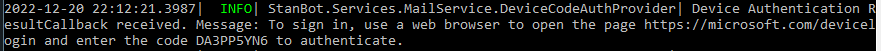
\includegraphics[width=1.3\textwidth]{img/Tut_deviceAuthLog.png}
    \caption{Anleitung - Device Authentication Log Message}
    \label{fig:tutorial-device-auth-log}
\end{figure}

\begin{figure}[h]
    \begin{minipage}[t]{0.5\textwidth}
        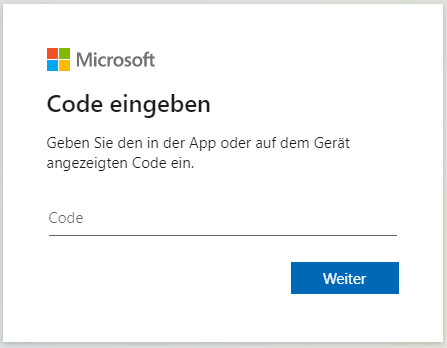
\includegraphics[width=0.8\textwidth]{img/Tut_deviceAuthLogin.png}
    \end{minipage}
    \begin{minipage}[t]{0.5\textwidth}
        \includegraphics[width=0.8\textwidth]{img/Tut_deviceAuthAccount.png}
    \end{minipage}
    \caption{Anleitung - Device Authentication}
    \label{fig:tutorial-device-auth}
\end{figure}

\newpage
\section{Besprechungsprotokolle}

\subsection{Kick Off Meeting 23.09.2022}

\subsubsection*{Anwesende Personen}

\begin{itemize}
    \item Markus Waldmann (WIPRO Betreuer, Dozent)
    \item Nicolas Wiedmer (WIPRO Arbeiter, Student)
    \item Yannis Krämer (WIPRO Arbeiter, Student)
    \item Martin Steiger (STAIR Präsident)
    \item Estefania Otero (STAIR Expräsidentin)
\end{itemize}

\subsubsection*{Besprochene Punkte}

\begin{enumerate}
    \item Der Aufbau der WIPRO Dokumentation mit den verschiedenen Kapitel
    \item Inhaltslänge wird mehr als 60 Seiten erwartet ausser die Dokumentation ist speziell kompakt.
    \item Yannis Krämer verlässt die Schweiz im Januar aufgrund eines Auslandsemesters. Alle beteiligten wären einverstanden damit die Präsentation frühzeitig oder online durchzuführen.
\end{enumerate}

\subsubsection*{Entscheidungen}

\begin{enumerate}
    \item Das Arbeitsjournal auf OneDrive soll von Anfang an freigegeben werden.
\end{enumerate}

\newpage
\subsection{Meeting mit STAIR 13.10.2022}

\subsubsection*{Anwesende Personen}

\begin{itemize}
    \item Yannis Krämer (WIPRO Arbeiter, Student)
    \item Martin Steiger (STAIR Präsident)
    \item Estefania Otero (STAIR Expräsidentin)
\end{itemize}

\subsubsection*{Besprochene Punkte}

\begin{enumerate}
    \item Es wurden verschiedene Architektur und Workflow Entscheidungen getroffen.
\end{enumerate}

\subsubsection*{Entscheidungen}

\begin{enumerate}
    \item Ein Student darf maximal einen Discord Account auf dem Server nützen. Der Account darf der Nutzer jedoch wechseln über die Zeit hinweg.
    \item Es braucht keinen Sync Job um manuelle Änderungen auf dem Server zu erkennen. STAIR Mitglieder müssen Anfangs instruiert werden, dass manuelle Änderungen, welche eigentlich vom Bot vorgenommen werden, nicht erlaubt sind. Dieses Feature wäre ein nice-to-have für die Zukunft.
    \item Der Übergang zum neuen Bot muss im Voraus den Studenten angekündigt werden. Eine Ankündigung per E-Mail wäre auch hilfreich, auch um Studenten auf den Discord Server zu bringen, welche diesen noch nicht genutzt haben. Es ist dabei aber okay, wenn sich die Studenten frisch anmelden müssen.
\end{enumerate}

\newpage
\subsection{Meeting mit Herr Waldmann 14.10.2022}

\subsubsection*{Anwesende Personen}

\begin{itemize}
    \item Markus Waldmann (WIPRO Betreuer, Dozent)
    \item Nicolas Wiedmer (WIPRO Arbeiter, Student)
    \item Yannis Krämer (WIPRO Arbeiter, Student)
\end{itemize}

\subsubsection*{Besprochene Punkte}

\begin{enumerate}
    \item Es wurde besprochen, wie die Dokumentation bezüglich Protokolle, Quelle und weiteren Inhalt und Format genau aussehen soll.
\end{enumerate}

\subsubsection*{Entscheidungen}

\begin{enumerate}
    \item Das Quellenformat, welches von Latex standardmässig genützt wird, darf so verwendet werden.
\end{enumerate}

\newpage
\subsection{Meeting mit STAIR 21.10.2022}

\subsubsection*{Anwesende Personen}

\begin{itemize}
    \item Yannis Krämer (WIPRO Arbeiter, Student)
    \item Martin Steiger (STAIR Präsident)
    \item Estefania Otero (STAIR Expräsidentin)
\end{itemize}

\subsubsection*{Besprochene Punkte}

\begin{enumerate}
    \item Diverse Entscheidungen bezüglich Stakeholder
\end{enumerate}

\subsubsection*{Entscheidungen}

\begin{enumerate}
    \item HSLU Mitarbeiter, welche gleichzeitig Studieren, dürfen weiterhin den Discord Server nützen.
    \item Masterstudenten dürfen den Discord Server ebenfalls nützen.
    \item Digital Ideation Studenten Fachrichtung Kunst gehören nicht zu STAIR und werden deshalb vom Discord Server ausgeschlossen.
    \item Das Aufsetzen des Servers und weitere Interaktionen über die Konsole sollen genau dokumentiert werden, da nicht alle (zukünftigen) STAIR Vorstandsmitglieder vertraut sind mit Konsolenanwendungen.
\end{enumerate}

\newpage
\subsection{Meeting mit Herr Waldmann 16.11.2022}

\subsubsection*{Anwesende Personen}

\begin{itemize}
    \item Markus Waldmann (WIPRO Betreuer, Dozent)
    \item Nicolas Wiedmer (WIPRO Arbeiter, Student)
    \item Yannis Krämer (WIPRO Arbeiter, Student)
\end{itemize}

\subsubsection*{Besprochene Punkte}

\begin{enumerate}
    \item Wenn Dinge, wie Clean Coding genutzt werden, dann muss dies aus der Dokumentation heraus auch ersichtlich sein.
    \item Der Aufbau des Testprotokolls wurde besprochen.
    \item Die Systemgrenzen müssen genau dokumentiert sein.
    \item Ein komischer Bug führte zu längeren Problemen und Verzögerungen in der Arbeit. Es wurden verschiedene Ansätze zur Lösung besprochen.
    \item Um deutsche Texte vom Computer korrigieren zu lassen, kann Microsoft Word, Adobe PDF Reader oder Thesaurus verwendet werden.
\end{enumerate}

\subsubsection*{Entscheidungen}

\begin{enumerate}
    \item Es wäre möglich, dass die E-Mails über das EnterpriseLab verschickt werden können. Es wurde beschlossen dort mal nachzufragen.
\end{enumerate}

\newpage
\subsection{Meeting mit STAIR 15.12.2022}

\subsubsection*{Anwesende Personen}

\begin{itemize}
    \item Nicolas Wiedmer (WIPRO Arbeiter, Student)
    \item Yannis Krämer (WIPRO Arbeiter, Student)
    \item Martin Steiger (STAIR Präsident)
\end{itemize}

\subsubsection*{Besprochene Punkte}

\begin{enumerate}
    \item Zeigen vom aktuellem Stand des Bots
    \item Erklärung der Umsetzung
\end{enumerate}

\subsubsection*{Entscheidungen}

\begin{enumerate}
    \item Bei der Authentifizierung soll eine vollständige Beispielmail dem User angezeigt werden um Missverständnisse zu verhindern.
    \item Es soll eine Fehlermeldung angezeigt werden beim Authorisierungsprozess, wenn die Domain der E-Mail falsch ist.
    \item Es soll eine Meldung dem Student angezeigt werden nach dem E-Mail verschicken, damit der Nutzer weiss, dass der Authentifizierungscode dem Stan geschickt werden muss.
    \item Es soll die Anzahl Accounts pro House angezeigt werden in der Statistik.
    \item Release soll zwischen den Semesterferien durchgeführt werden, damit es keine Probleme in der Prüfungsphase gibt.
\end{enumerate}

\newpage
\subsection{Meeting mit Herr Waldmann 21.12.2022}

\subsubsection*{Anwesende Personen}

\begin{itemize}
    \item Markus Waldmann (WIPRO Betreuer, Dozent)
    \item Nicolas Wiedmer (WIPRO Arbeiter, Student)
    \item Yannis Krämer (WIPRO Arbeiter, Student)
\end{itemize}

\subsubsection*{Fragen}

\begin{enumerate}
    \item Wie lange soll die Präsentation werden?
        \begin{itemize}
            \item Die Präsentation sollte etwa 20 Minuten dauern. Wenn die Präsentation noch eine Demonstration beinhaltet, dann sollte diese 25 Minuten dauern.
        \end{itemize}
    \item Was soll der Inhalt der Präsentation sein?
        \begin{itemize}
            \item Die Präsentation soll den Werdegang des Projektes aufzeigen.
            \item Die Präsentation soll das Produkt, wie in einem Pitch, verkaufen.
            \item Der genaue Auftrag soll nochmals Aufgezeigt werden.
            \item Die Umsetzung soll die Herausforderungen und die davon resultierenden Masnnahmen und Lösungen aufzeigen.
        \end{itemize}
    \item Geht 9. oder 10. Januar als Präsentationstermin?
        \begin{itemize}
            \item Nicolas Wiedmer, Yannis Krämer und Martin Steiger haben an beiden Tagen Zeit.
            \item Estefania Otero hat am 10. nur am Morgen Zeit.
            \item Yannis Krämer ist ab 15. Januar im Ausland aufgrund eines Auslandsemesters.
            \item Markus Waldmann hat an beiden Tagen Zeit
        \end{itemize}
    \item Wo soll man das Arbeitsjournal einfügen?
        \begin{itemize}
            \item Der Aufwand muss aufgezeigt werden, damit man sieht das die Credits gerechtfertigt sind.
            \item Der Unterschiedzwischen der soll und ist Situation.
            \item Eine Seite pro Person ist ausreichend.
        \end{itemize}
    \item Letzte Tipps
        \begin{itemize}
            \item Bewertungsraster nochmals anschauen
            \item Überall auf den Kontrast achtenund keine rot/grüne Designs verwenden.
            \item Die Kopf und Fusszeile sollen mindestens der Titel der Arbeit und die Seitenzahl beinhalten. Optimal wäre noch wenn das Kapitel erwähnt wird.
        \end{itemize}
\end{enumerate}

\subsubsection*{Besprochene Punkte}

\begin{enumerate}
    \item Der zweite Experte ist Bruno Joho.
\end{enumerate}

\subsubsection*{Entscheidungen}

\begin{enumerate}
    \item Das Glossar soll nach dem Abstract eingefügt werden.
    \item Die detailierten Testprotokolle sollen im Anhang hinzugefügt werden. Eine Zusammenfassung von den Ergebnissen soll in den Hauptteil eingefügt werden.
    \item Das Abstract soll auf Deutsch und Englisch eingefügt werden.
    \item Die Abgabe soll wenn möglich per E-Mail erfolgen an alle beteiligten, welche auch an der Präsentation teilnehmen werden.
    \item Die Besprechungsprotokolle müssen vor allem die Entscheidungen und die dazugehörigen Begründungen beinhalten.
\end{enumerate}

\end{document}
